\documentclass[conference]{IEEEtran}
\IEEEoverridecommandlockouts
% The preceding line is only needed to identify funding in the first footnote. If that is unneeded, please comment it out.
\usepackage{cite}
\usepackage{amsmath,amssymb,amsfonts}
\usepackage{algorithmic}
\usepackage{graphicx}
\usepackage{bussproofs}
\EnableBpAbbreviations
\usepackage{hyperref}
\usepackage{tikz,pgfplots}
\pgfplotsset{compat=newest}
\usepackage{tikz-cd}
\usepackage{textcomp}
\usepackage{xcolor}
\usepackage{amsthm}
\usepackage{caption}
\usepackage{subcaption}
\usetikzlibrary{cd}
\usepackage{mathabx}
\usepackage{cmll}
\usepackage{stmaryrd}



% MATH TEXT STYLES
\newcommand{\B}[1]{\mathbf{#1}}
\newcommand{\BB}[1]{\mathbb{#1}}
\newcommand{\C}[1]{\mathcal{#1}}
\newcommand{\F}[1]{\mathfrak{#1}}
\newcommand{\TT}[1]{\mathtt{#1}}
\newcommand{\RM}[1]{\mathrm{#1}}
\newcommand{\SF}[1]{\mathsf{#1}}



%CATEGORIES

\newcommand{\Met}{\mathsf{Met}}
\newcommand{\Mod}{\Lawv\mathsf{Mod}}
\newcommand{\GMet}{\Lawv\mathsf{CCat}}
\newcommand{\Fun}{\mathsf{Fun}}
\newcommand{\colim}{\mathrm{colim}}
\newcommand{\Yon}{\B{Y}}
\newcommand{\Hom}{\mathrm{Hom}}
\newcommand{\Sym}{\mathrm{Sym}}
\newcommand{\matr}[1]{\hat{#1}}

\newcommand\pfun{\mathrel{\ooalign{\hfil$\mapstochar\mkern5mu$\hfil\cr$\to$\cr}}}



% LAMBDA CALCULI

\newcommand{\lamcalc}{$\lambda$-calculus}
\newcommand{\lam}{\lambda}

\newcommand{\STLC}{\RM{STLC}}
\newcommand{\BSTLC}{\mathsf b\RM{STLC}}
\newcommand{\RSTLC}{\C R\RM{STLC}}
\newcommand{\STDLC}{\RM{ST}\partial\RM{LC}}
\newcommand{\Real}{\SF{Real}}

\newcommand{\Der}{\SF D}
\newcommand{\To}{\Rightarrow}

\newcommand{\finMS}[1]{\C M_{\RM{fin}}(#1)}

\newcommand{\true}{\RM{True}}
\newcommand{\false}{\RM{False}}
\newcommand{\bool}{\SF{Bool}}

\newcommand{\Te}[1]{\C T(#1)}




% METRIC STUFF
\newcommand{\Lawv}{\BB L}
\newcommand{\QualREL}[1]{#1 \SF{Rel}}
\newcommand{\QREL}{\QualREL{Q}}
\newcommand{\LREL}{\QualREL{\Lawv}}
\newcommand{\LCAT}{\Lawv\SF{CCat}}

\newcommand{\op}{\mathrm{op}} 
\newcommand{\sk}{\mathrm{sk}} 
\newcommand{\sym}{\mathrm{sym}} 
\newcommand{\menus}{\dotdiv} 

\newcommand{\norm}[1]{\lVert#1\rVert}
\newcommand{\supnorm}[1]{\lVert#1\rVert_\infty}
\newcommand{\absv}[1]{\left\lvert#1\right\rvert}

% TROPICAL STUFF

\newcommand{\trop}[1]{\SF t #1}
\newcommand{\model}[1]{\llbracket#1\rrbracket}
\newcommand{\nodel}[1]{\langle #1\rangle}
\newcommand{\sumt}[1]{{+}^{#1}}
\newcommand{\prodt}[1]{{\times}^{#1}}


% MISCELLANEOUS

\newcommand{\HOM}[3]{{#1}(#2,#3)}
\newcommand{\N}{\BB N}
\newcommand{\R}{\BB R}
\newcommand{\set}[1]{\{#1\}}
\newcommand{\multiset}{\C M_{\mathrm{fin}}}

\newcommand{\eps}{\epsilon}

\newcommand{\twoheaddownarrow}{\mathrel{\rotatebox[origin=c]{270}{$\twoheadrightarrow$}}\!}


%MATH EVIRONMENTS

\newtheorem{example}{Example}
\newtheorem{definition}{Definition}
\newtheorem{problem}{Problem}
\newtheorem{notation}{Notation}

\newtheorem{remark}{Remark}
\newtheorem{theorem}{Theorem}
\newtheorem{conjecture}{Conjecture}

\newtheorem{lemma}[theorem]{Lemma}

\newtheorem{proposition}[theorem]{Proposition}
\newtheorem{result}{Result}
\newtheorem{fact}{Fact}


\newtheorem{corollary}[theorem]{Corollary}



\def\BibTeX{{\rm B\kern-.05em{\sc i\kern-.025em b}\kern-.08em
    T\kern-.1667em\lower.7ex\hbox{E}\kern-.125emX}}
\begin{document}

\title{Tropical Mathematics and the Lambda Calculus}

%\author{\IEEEauthorblockN{Davide Barbarossa}
%\IEEEauthorblockA{\textit{Universit\`a di Bologna}\\
%Bologna, Italy \\
%davide.barbarossa@unibo.it}
%\and
%\IEEEauthorblockN{Paolo Pistone}
%\IEEEauthorblockA{\textit{Universit\`a Roma Tre}\\
%Rome, Italy\\
%paolo.pistone@uniroma3.it}
%}

\maketitle

\begin{abstract}
In this paper we study an interpretation of the $\lambda$-calculus in the framework of tropical mathematics, and we show that it provides a unified framework for both 
program metrics, as based on the analysis of program sensitivity via Lipschitz-conditions, and for resource analysis, as based on higher-order program differentiation.
We discuss applications of this tropical semantics to ``best case'' resource analysis as well as to other quantitative properties like convergence log-probabilities and differential privacy.
Finally, we show that a general foundation for this semantic approach is provided by an abstract correspondence between Lawvere's theory  
of generalized metric spaces and tropical algebra.



\end{abstract}

\begin{IEEEkeywords}
Differential lambda calculus, Tropical semiring, Lawvere quantale, Program metrics, Relational semantics.
\end{IEEEkeywords}

\section{Introduction}

In recent years, more and more interest in the programming language community has been directed towards the study of \emph{quantitative} properties of programs like e.g.~computing the number of computation steps, or convergence probabilities, 
as opposed to purely \emph{qualitative} properties like e.g.~termination or program equivalence. 
Notably, a significant effort has been made to extend, or adapt, well-established qualitative methods, like e.g.~type systems, relational logics or denotational semantics, to account for quantitative properties. We can mention, for example, 
intersection type systems aimed at capturing time or space resources \cite{decarvalho2018, Accattoli2022} or convergence probabilities \cite{Breuvart2018, PistoneLICS2022},  relational logics to account for probabilistic properties like e.g.~differential privacy \cite{Barthe_2012} or metric preservation \cite{Reed2010, dallago}, as well as the study of denotational models for 
probabilistic \cite{Ehrhard2011, Staton2017} or differential \cite{difflambda} extensions of the $\lambda$-calculus. 
The main reason to look for methods relying on (quantitative extensions of) type-theory or denotational semantics is that these approaches yield \emph{modular} and \emph{compositional} techniques, that is, allow one to deduce properties of complex programs from the properties of their constituent parts.   

\subsection{Two kinds of quantitative approaches}

Among such quantitative approaches, two different directions have received considerable attention. 

On the one hand one there is the approach of \emph{program metrics} \cite{Reed2010, Gaboardi2017, Gabo2019} and \emph{quantitative equational theories} \cite{Plotk}: when considering probabilistic or approximate computation, rather than asking whether two programs compute \emph{the same} function (which is rarely the case), it makes more sense to ask   whether they compute functions which do not differ \emph{too much}. This has motivated the study of denotational frameworks in which types are endowed with a metric, measuring similarity of behavior; this approach has found  applications in e.g.~differential privacy \cite{Reed2010} and coinductive methods \cite{Bonchi2018}, and was recently extended to account for the full $\lambda$-calculus \cite{Geoffroy2020, PistoneLICS, PistoneFSCD2022}.

On the other hand, there is the approach based on \emph{differential} \cite{difflambda} or \emph{resource-aware} \cite{Boudol1993} extensions of the $\lambda$-calculus, which is well-connected to the so-called \emph{relational semantics} \cite{Manzo2012, Manzo2013, dill} and has a syntactic counterpart in the study of \emph{non-idempotent} intersection types \cite{decarvalho2018, Mazza2016}. This family of approaches have been exploited to account for higher-order program differentiation \cite{difflambda}, to establish reasonable \emph{cost-models} for the $\lambda$-calculus \cite{Accattoli2021}, and have also been shown suitable for the probabilistic setting \cite{Manzo2013, Breuvart2018, PistoneLICS2022}. 


In both approaches the notion of \emph{linearity}, in the sense of linear logic \cite{girardLl} (i.e.~of using inputs exactly once), plays a crucial role.
In metric semantics, linear programs correspond to \emph{non-expansive} maps, that is, to functions that do not increase distances; moreover, the possibility of duplicating inputs leads to interpret \emph{bounded} programs (i.e.~programs with a fixed duplication bound) as \emph{Lipschitz-continuous} maps \cite{Gaboardi2017}.
By contrast, in the standard semantics of the differential $\lambda$-calculus, linear programs correspond to linear maps, in the usual algebraic sense, while the possibility of duplicating inputs leads to consider functions defined as \emph{power series}.


A natural question is thus whether these two apparently unrelated ways of interpreting linearity and duplication can be somehow reconciled. At a first glance, there seems to be a  ``logarithmic'' gap between the two approaches:
in metric models $n$ times duplication results in a \emph{linear} (hence Lipschitz) function $n\cdot x$, while in differential models this results in a \emph{polynomial} function $x^{n}$, hence not Lipschitz. The fundamental motivation of this work is then the observation that 
this gap is naturally overcome once we interpret these functions in the framework of tropical mathematics, where, as we'll see, the monomial $x^{n}$ ``reads as'' the linear function $n\cdot x$.

% from higher-order programs is based on  soon as one develops  differential semantics in the framework of 
%tropical mathematics.
%
%''
%
%s
%emantics a typical ``duplicating'' map is obtained by composing the diagonal with multiplication:
%$$
%\begin{tikzcd}
%\mathbb R \ar{rrr}{x\mapsto \langle x, x\rangle}
% & &  &
% \mathbb R\times \mathbb R 
% \ar{rrr}{\langle x,y\rangle \mapsto x\cdot y}
% & & & \mathbb R
%\end{tikzcd}
%$$
%yielding the square product function $\lambda x.x^{2}$.
%However, in metric semantics this function needs not even exist (as these models are often restricted to Lipschitz-continuous maps \cite{Gabo2017})! Instead, a typical ``duplicating'' map can be obtained by composing the diagonal with the sum 
%$$
%\begin{tikzcd}
%\mathbb R \ar{rrr}{x\mapsto \langle x, x\rangle}
% & &  &
% \mathbb R\times \mathbb R 
% \ar{rrr}{\langle x,y\rangle \mapsto x+y}
% & & & \mathbb R
%\end{tikzcd}
%$$
%yielding the linear (and Lipschitz) function $\lambda x.2x$.
%
%As this example seems to suggest, there seems to be a sort of ``logarithmic'' gap between the two approaches. Can this be made explicit?



\subsection{Tropical mathematics and program semantics } 


Tropical mathematics was introduced in the seventies by the Brazilian mathematician Imre Simon \cite{Simon} as an alternative approach to algebra and geometry where the usual ring structure of numbers based on addition and multiplication is replaced by the semiring structure given, respectively, by ``$\min$'' and ``$+$''.
%
%
% interpreting the usual ``$\times$'' and  ``$+$'' operations by  ``$+$'' by ``$\min$''. It can thus be seen as a sort of ``logarithmic'' version of usual geometry (this idea can be made precise via the so-called \emph{Maslov deformation} \cite{}).
%Tropical mathematics is a form of \emph{idempotent} mathematics, since the role of addition is 
%played by the idempotent operation $\min$.
For instance, the polynomial $p(x,y)=x^{2}+xy^{2}+y^{3}$, when interpreted over the tropical semiring, translates as the piecewise linear function
$
\varphi(x,y)=\min\{2x, x+2y, 3y\}
$.

%This is not a \emph{ad-hoc} setting: 
In the last decades, tropical geometry evolved into a vast and rich research domain, providing a combinatorial counterpart of usual algebraic geometry, with important connections with optimisation theory \cite{Sturmfelds}.
Computationally speaking, working with $\min$ and $+$ is generally easier than working with standard addition and multiplication; for instance, the fundamental (and generally intractable) problem of finding the roots of a polynomial admits a \emph{linear time} algorithm in the tropical case (and, moreover,  the tropical roots can be used to approximate the actual roots \cite{Noferini2015}).
The computational nature of tropical notions explains why these are so widely applied in computer science, notably for convex analysis and machine learning (see \cite{Maragos2021} for a recent survey).

Coming back to our previous discussion on program semantics, tropical geometry might seem to provide precisely what we are looking for, as it turns the monomials $x^{n}$ into the Lipschitz functions $n\cdot x$.
At this point, it is worth mentioning that a tropical variant of relational semantics has already been considered \cite{Manzo2013}, and shown capable of capturing \emph{best-case} quantitative properties, but has not yet been studied in detail. Furthermore, connections between tropical linear algebra and metric spaces (in the abstract setting of \emph{quantale-enriched} categories \cite{Hofmann2014, Stubbe2014}), have also been observed \cite{Fuji}.

In this paper we demonstrate that the relational interpretation of the $\lambda$-calculus based on tropical mathematics does indeed provides the desired bridge between differential and metric semantics. Moreover, we show that the conceptual unification of these two approaches suggests ways in which techniques from resource-analysis could be used in sensitivity analysis and \emph{vice-versa}, paving the way for new  applications of tropical geometry to the  study of higher-order programs.


\subsection{Contributions}

Our contributions in this paper are threefold:
\begin{itemize}

\item we study the relational model over the tropical semiring  and we show that the functions interpreting simply-typed lambda terms, which correspond to a generalization of \emph{tropical Laurent series} \cite{Porzio2021}, are locally Lipschitz-continuous, thus yielding a full-scale metric semantics for the $\lambda$-calculus and its bounded fragments. This is in Sections \ref{section3} and \ref{section4}.
%Moreover, we exploit the differential structure of the relational model to study the \emph{tropical Taylor expansion} of a $\lambda$-term, which can be seen as an approximation of the term by way of Lipschitz-continuous maps.


\item Using the relational model as our main source of inspiration,  we suggest a few potential applications of tropical methods to the study of quantitative properties of non-deterministic and probabilistic functional programs, like counting best-case computation steps, 
measuring convergence log-probabilities, and 
differential privacy. This is in Section~\ref{section5}

\item We conclude 
by putting the connection between the 
tropical, differential and metric viewpoints at the right level of generality.
By recalling and suitably extending a well-known correspondence between Lawvere's \emph{generalized metric spaces} \cite{Lawvere1973, Stubbe2014} and modules over the tropical semi-ring \cite{Russo2007}, we show that the category of \emph{complete} generalized metric spaces provides a model of the differential $\lambda$-calculus which extends the tropical relational model. This is in Section~\ref{section6}.
\end{itemize}
%
%\section{Bounded and Differential $\lambda$-Calculi}
%
%
%Bounded Simply Typed $\lambda$-calculus $\BSTLC$:
%$$
%A::= o \mid !_{n}A \multimap A
%$$
%
%
%Resource Simply Typed $\lambda$-calculus $\RSTLC$:
%$$
%A::= o \mid [A, \dots , A] \multimap A
%$$
%
%
%Define a translation of types $(-)^{\C R}$ from $\BSTLC$ to $\RSTLC$ by $o^{\C R}=o$ and $(!_{n}A\multimap B)^{\C R}=
%[\underbrace{A^{\C R},\dots, A^{\C R}}_{n\text{ times}}]\multimap B^{\C R}$.
%
%\begin{proposition}
%$\Gamma \vdash_{\BSTLC} M:A$ implies 
%$\Gamma^{\C R}\vdash_{\RSTLC}M:A^{\C R}$.
%\end{proposition}
%





\section{A Bridge Between Two Quantitative Approaches to the $\lambda$-calculus}\label{section2}



%Recall the two approaches with more details on lambda-calculus and on existing challenges.


%In this section, we discuss in some more detail the two approaches to quantitative semantics we mentioned in the Introduction, at the same time providing an overview of how we aim at bridging them using tropical mathematics.

\paragraph*{Controlled duplication/erasure via graded types: bounded $\lambda$-calculus $\BSTLC$}\label{sec:BSTLC}

One can see that the comonad $!$ of $\LREL$ can be ``decomposed'' {\color{red}REF} into a family of ``graded exponentials functors'' $!_n:\LREL\to\LREL$ ($n\in\BB N$), defined on objects by taking multisets of cardinality \emph{at most} $n$. %  lift to functors 
The sequence $(!_n)_{n\in\N}$ gives rise to a so-called \emph{$\N$-graded linear exponential comonad} on (the SMC) $\LREL$. %satisfying the adjunction: $\LREL(Z\otimes !_{n}X,Y) \simeq \LREL(Z, !_{n}X\multimap Y)$.

As such, $(\LREL,(!_n)_{n\in\N})$ is a model of graded calculi ensuring bounded duplications via graded typing systems, for instance it is a model  \cite{Katsumata2018} of the language $\BSTLC$, a simplified version of the language $\mathrm{Fuzz}$ \cite{Reed2010}, defined as follows: 
the terms are as for the $\STLC$, the types are $A::= * \ \mid  \ !_{n}A \multimap A$, the contexts of the typing judgements are sets of declarations of the form $x :_{n}A$, with $n\in \mathbb N$, and the typing rules are: %given in Fig.~\ref{fig:rules}
	\[ \scriptsize \arraycolsep=5pt\def\arraystretch{2.8}
	\begin{array}{cccc}
		\prooftree
		\Gamma \vdash M:A
		\justifies
		\Gamma, x:_{0}B \vdash M:A
		\endprooftree 
		&
		\prooftree
		\Gamma, x:_{n}B, y:_{m} B\vdash M:A
		\justifies
		\Gamma, x:_{n+m}B\vdash M\{x/y\}:A
		\endprooftree 
		&
		\prooftree
		\Gamma, x:_{n} A\vdash M: B
		\justifies
		\Gamma\vdash \lambda x.M: !_{n}A\multimap B
		\endprooftree
		&
		\prooftree
		\Gamma \vdash M: !_nA\multimap B
		\quad
		\Delta\vdash N: A
		\justifies
		\Gamma +n\Delta\vdash MN: B
		\endprooftree
	\end{array}
	\]
where $\Gamma+\Delta$ is defined letting $(\Gamma, x:_{m} A)+( \Delta, x:_{n} A) =  (\Gamma+\Delta), x:_{m+n}A$, and $m\Gamma$ is made all $x:_{mn}A$ for $(x:_{n}A) \in \Gamma$.  
The axiom is $x:_{1}A\vdash x: A$.
The main feature of this language is that if $\vdash \lambda x.M:\,!_nA\multimap B$, then $x$ is duplicated at most $n$ times in the reduction of $\vdash (\lambda x.M)N :B$ to the normal form.
%E.g., $\vdash_{\BSTLC} \lambda {\color{red}z}.\left( \lambda x{\color{green}y}. yxx \right)z : \, !_{\color{red}2} *\multimap !_{\color{green}1}(!_{\color{violet}1} * \multimap !_{\color{blue}1} * \multimap *) \multimap *$.
%Observe that one can always type an affine term like e.g.~$\lambda xy.x$ with a linear type $A\multimap B\multimap A$. Instead, a term like $\lambda xy.x(xy)$ containing two occurrences of $x$ cannot be given the linear type $(A\multimap A)\multimap (A\multimap A)$ but a type of the form
%$!_{2}(A\multimap A)\multimap (A\multimap A)$. 

%\begin{remark}\label{rmk:ModelsOfBSTLC}
%Similarly to It is known {\color{red}(([reference??] e dire meglio)} 

Remark that since arrow types are interpreted via $\model{!_{n}A\multimap B}:= !_{n}\model A \times \model B$, 
if $\model *$ is finite, then $\model{A}$ is a finite set for any type $A$ of $\BSTLC$.
%\end{remark}
%Bounded types are interesting because of the following proposition:
%\begin{proposition}
%For all bounded types $A,B$, the morphisms from $\model A$ to $\model B$ (in all parametric relational models) correspond to polynomials.
%\end{proposition}
%\begin{proof}
%It suffices to check that $\model A$ is finite for all bounded types $A$. Indeed this implies that a morphism $t:\model A\to \model B$ is a finite matrix $t: \model A \times \model B \to \Lawv$.Hence, its corresponding map $\widehat t:\Lawv^{\model A} \to \Lawv^{\model B}$ is a polynomial.
%\end{proof}

%For example (here $!_{n}(\Lawv^{X}):= \Lawv^{\C M_{\leq n}(X)}$):
%\begin{itemize}
%\item a map $f\in \LREL( !_{1}\Lawv, \Lawv)$ is of the form $f(x)=\min \{x+a,b\}$;
%\item a map $f\in \LREL(!_{2}\Lawv, \Lawv)$ is a ``quadratic'' polynomial $f(x)=\min\{2x+a, x+b, c\}$.
%\end{itemize}

\begin{comment}

\begin{figure*}

	\scriptsize
	
	\[ \arraycolsep=5pt\def\arraystretch{2.8}
	\begin{array}{cccc}
		\prooftree
		\Gamma \vdash M:A
		\justifies
		\Gamma, x:_{0}B \vdash M:A
		\endprooftree 
		&
		\prooftree
		\Gamma, x:_{n}B, y:_{m} B\vdash M:A
		\justifies
		\Gamma, x:_{n+m}B\vdash M\{x/y\}:A
		\endprooftree 
		&
		\prooftree
		\Gamma, x:_{n} A\vdash M: B
		\justifies
		\Gamma\vdash \lambda x.M: !_{n}A\multimap B
		\endprooftree
		&
		\prooftree
		\Gamma \vdash M: !_nA\multimap B
		\quad
		\Delta\vdash N: A
		\justifies
		\Gamma +n\Delta\vdash MN: B
		\endprooftree
		\\
		\\
		\hline
		\\
		\prooftree
		\Gamma, x: A\vdash M: B
		\justifies
		\Gamma\vdash \lambda x.M: A\to B
		\endprooftree 
		&
		\prooftree
		\Gamma \vdash M: A\to B
		\quad
		\Gamma\vdash \mathbb T: A
		\justifies
		\Gamma \vdash M\mathbb T: B
		\endprooftree 
		&
		\prooftree
		\Gamma \vdash M: A\to B
		\quad
		\Gamma \vdash N: A
		\justifies
		\Gamma \vdash \Diff{M}{N}: A\to B
		\endprooftree
		&
		\prooftree
		\Gamma\vdash M_1: A
		\,\cdots\,
		\Gamma \vdash M_n:A
		\justifies
		\Gamma \vdash M_1+\cdots +M_n : A
		\using (n\geq 2)
		\endprooftree
	\end{array}
	\]
	\caption{Typing rules (axiom rules are given in the text) for $\BSTLC$ (top) and $\STDLC$ (bottom).}\label{fig:rules}
\end{figure*}

\end{comment}

\paragraph*{Controlled duplication/erasure via resources: the differential $\lambda$-calculus $\STDLC$}\label{sec:STDLC}

A Cartesian closed differential $\lambda$-category (CC$\partial\lambda$C)\cite{Manzo2010,Blute2009, Blute2019} is a CCC enriched over commutative monoids %(i.e.\ we can add morphisms and there is a $0$ morphism)
%, it is Cartesian closed%(with the closed structure compatible with the additive structure)
and equipped with a certain \emph{differential operator} $D$, generalising the usual notion of differential, see e.g.\ \cite{BluteEhrhTass10}.
%An example is the CC$\partial\lambda$C of convenient vector spaces with smooth maps, where $D$ is the ``real'' differential $Df:\mathbb{V}\times\mathbb{V}\rightarrow \mathbb{W}$, $Df(x,u):=\dfrac{d}{dt}{\!\Big|_{t=0}} f(x+tu)$, of smooth maps $f:\mathbb{V}\rightarrow \mathbb{W}$.
%More precisely, a cartesian category $\C C$ is a $C\partial C$ when:
%\begin{itemize}
%\item $\C C$ is left-additive, i.e.~its hom-sets have the structure of commutative monoids, and the cartesian structure is well-behaved w.r.t.~this monoid structure;
%\item $\C C$ is equipped with a differential operator $D:
%\C C(X,Y)\to \C C(X\times X,Y)$ satisfying some axioms which capture usual properties of differentials (e.g.~the linearity of $D$ in one of its two variables, the chain rule, etc.).
%\end{itemize}
Now, applying \cite[Theorem 6.1]{lemay2020} one can check that
%\begin{proposition}[{\color{red}LEMAY??}]\label{thm:LREL!CCDC}
 $\LREL_!$ becomes a CC$\partial\lambda$C when equipped with the \emph{tropical differential operator} $D:\HOM{\LREL}{!X}{Y}\to \HOM{\LREL}{!(X\& X)}{Y}$ defined as $(Dt)_{\mu\oplus\rho,b}=t_{\rho+\mu,b}$ if $\#\mu=1$ and as $\infty$ otherwise (using the iso $(\mu,\rho)\in !Z\times !Z'\mapsto\mu\oplus\rho \in !(Z+Z')$).
%\end{proposition}
%\begin{remark}For $t\in\HOM{\LREL}{!X}{Y}$, we have: $D^2 t\in\HOM{\LREL_!}{(X+X)+(X+X)}{Y}$, where $(D^2 t)_{(\rho\oplus\rho')\oplus(\nu\oplus\nu'),b}$ equals $t_{\nu+\nu'+\rho',b}$ if $\rho=\emptyset$ and $\#\rho'=1=\#\nu$; it equals $t_{\rho+\nu',b}$ if $\rho'=\emptyset=\nu$ and $\#\rho=1$; it equals $\infty$ otherwise.\end{remark}
%This ensures that one can define a sound interpretation of $\STDLC$-terms in the standard way (see [Section 4.3, \cite{Manzo2010}]).

As such, $(\LREL_!,D)$ is a model of the differential $\lambda$-calculus $\STDLC$ \cite{ER}, a language ensuring exact control of duplications via a notion of linear substitution.
Its syntax (e.g.\ \cite[Section 3]{Manzo2010}) is given by the \emph{terms} $M$ and the \emph{sums} $\mathbb T$, mutually generated by: $M::= x\mid \lambda x.M \mid M\mathbb T \mid \Diff{M}{M}$ and $\mathbb T::= 0 \mid M \mid M+\mathbb T$,
quotiented by $\alpha$-equivalence, by equations that make $+,0$ form a commutative monoid on the set of sums, %, i.e.\ commutativity and associativity of $+$ and neutrality of $0$ w.r.t.\ $+$;
by linearity of $\lam x.(\_)$, $\Diff{\_}{\_}$ and $(\_)\mathbb T$ (but \emph{not} of $M(\_)$) and by irrelevance of the order of consecutive $\Diff{\_}{\_}$.
%Remark that $M(\_)$ is \emph{not} set to be linear: $\lambda x.0=0\mathbb T=\Diff{0}{N}=\Diff{M}{0}=0$ but $M0\neq0$ in general.
%This is crucial for the definition of the Taylor expansion.
We follow the tradition of quotienting also for the idempotency of $+$.
%Sums are, then, just \emph{finite} sets of terms.
The types are $A::= *\mid A\to A$, the typing rules: %in Figure~\ref{fig:rules}
	\[ \scriptsize \arraycolsep=5pt\def\arraystretch{2.8}
	\begin{array}{cccc}
		\prooftree
		\Gamma, x: A\vdash M: B
		\justifies
		\Gamma\vdash \lambda x.M: A\to B
		\endprooftree 
		&
		\prooftree
		\Gamma \vdash M: A\to B
		\quad
		\Gamma\vdash \mathbb T: A
		\justifies
		\Gamma \vdash M\mathbb T: B
		\endprooftree 
		&
		\prooftree
		\Gamma \vdash M: A\to B
		\quad
		\Gamma \vdash N: A
		\justifies
		\Gamma \vdash \Diff{M}{N}: A\to B
		\endprooftree
		&
		\prooftree
		\Gamma\vdash M_1: A
		\,\cdots\,
		\Gamma \vdash M_n:A
		\justifies
		\Gamma \vdash M_1+\cdots +M_n : A
		\using (n\geq 2)
		\endprooftree
	\end{array}
	\]
where a context $\Gamma$ is a list of typed variable declarations.
The axioms are $\Gamma, x:A \vdash x: A$ and $\Gamma\vdash 0:A$.
The main feature of this language is that $\Der^n[\lambda x.M,N^n]0$ has a non-zero normal form iff $x$ is duplicated exactly $n$ times during the reduction to normal form.
%In $\BSTLC$ the typing system handles duplications; in $\STDLC$ the syntax with its operational semantics (that we do not give) does it.
\begin{comment}
Writing $\Der^2[\_,(\_)^2]$ as a shortcut for $\Der[\Der[\_,\_],\_]$ and $\Der^1[\_,(\_)^1]$ for $\Diff{\_}{\_}$, the analogue of the previous $\BSTLC$-term is $\vdash_{\STDLC} \lambda {\color{red}z}. \Der^{\color{red}2}[
	\lambda x{\color{green}y}.
		\Der^{\color{violet}1} [
				\Der^{\color{blue}1} [y, x^{\color{blue}1}]
        0, x^{\color{violet}1}
	]0
, z^{\color{red}2}]0
: {\color{red}*}\to ({\color{green}* \to * \to *}) \to *$.
%Here we wrote $\Der^2[\_]\cdot (\_)^2$ as a shortcut for $\Der[\Der[\_]\cdot (\_)]\cdot (\_)$ and $\Der^1[\_]\cdot (\_)^1$ for $\Der[\_]\cdot (\_)$.
In particular, if the \emph{multiplicities} of the arguments (the colored exponents) do not exactly match the number of duplications, e.g.\ in $\vdash_{\STDLC} \lambda z. \Der^{\color{red}3}[
	\lambda xy.
		\Diff{
				\Diff{y}{x}
		0}{x}
	0
, z^{\color{red}3}]0
: *\to (* \to * \to *) \to *$, then the term reduces to the empty sum $0$ (representing an \emph{error}).
\end{comment}
%Correspondingly, the syntax of the simply typed \emph{differential} $\lambda$-calculus ($\STDLC$) is defined by enriching $\STLC$ with a monoid structure $0,+$ over terms, as well as with $\Der$ and a notion of \emph{linear substitution} (see \cite{difflambda} or the Appendix for details).

%Until now we simply specialised well-known results in our tropical case, with the intent of showing how things read in this particular case.
%Now we go further, by showing that $\LREL_!$ actually admits a \emph{differential structure}, turning it into a model of the $\STDLC$, i.e.~a $CC\partial C$.
%This viewpoint
%, is where the \emph{metric} and the \emph{differential} viewpoints converge, as explained in the Introduction and Section II, and it % will be further generalised in Section \ref{section6}.

%A model of the $\STDLC$ is usually understood as so-called \emph{Cartesian closed differential categories} (CC$\partial$C), see \cite{Manzo2012} for details.
%In order to treat the $+$ and the constructor $D[\_]\cdot (\_)$ of $\STDLC$, the main features of a CC$\partial$C $\C C$ are that:
%
%1) $\C C$ is a left-additive-CCC, i.e.\ its Homsets are commutative monoids and its Cartesian closed structure is well behaved w.r.t.\ this monoid structure;
%
%2) $\C C$ is equipped with a differential operator map $D:\HOM{\C C}{X}{Y}\to \HOM{\C C}{X\times X}{Y}$ (here $\times$ is the Cartesian product of $\C C$) satisfying $8$ axioms, called D1, ..., D7, D-curry.

%Let us show the differential structure of $\LREL_!$ (remember that the Cartesian product of $\LREL_!$ is the disjoint union $+$).

%\begin{definition} The \emph{tropical differential operator} is the map $D:\HOM{\LREL}{!X}{Y}\to \HOM{\LREL}{!(X+X)}{Y}$ defined as $(Dt)_{\mu\oplus\rho,b}=t_{\rho+\mu,b}$ if $\#\mu=1$ and as $\infty$ otherwise (where a multiset $\nu \in !(X+X)$ is identified with a disjoint sum of $\mu,\rho\in !X$).\end{definition}

%The models of $\STDLC$ are the cartesian \emph{closed} differential categories ($CC\partial C$), which are defined as $C\partial C$ which are also cartesian closed, and in which the monoid structure and the differential operator are both well-behaved with respect to the closed structure \cite{Manzo2012}. 


 



%\section{Tropical (non-)Linear Algebra and computation}
\section{The Tropical Relational Model
%Tropical mathematics%: a possible synthesis
}\label{section3}
Now, what about the good old, ``unbounded'', simply typed $\lambda$-calculus? Actually, by using unbounded duplications, one might lose the Lipschitz property. For instance, while the functions $M_{k}=\lambda x. k\cdot x: \BB R\to \BB R$ are all Lipschitz-continuous, with Lipschitz constant $k$, the function $M=\lambda x.x^{2}$ obtained by ``duplicating'' $x$ is not Lipschitz anymore: $M$ is, so to say, \emph{too} sensitive to errors. 
More abstractly, it is well-known that the category $\Met$ is \emph{not} cartesian closed, so it is not a model of $\STLC$ (yet, several cartesian closed \emph{sub-}categories of $\Met$ do exist, see e.g.~\cite{Clementino2006, PistoneFSCD2022}).
Still, one might observe that the program $M$ above is actually Lipschitz-continuous, if not globally, at least \emph{locally} (i.e.~over any compact set). Indeed, some cartesian closed categories of locally Lipschitz maps have been produced in the literature \cite{Ehrhard2011, PistoneLICS}, and a new example will be exhibited in this paper.

At this point, as the Taylor formula decomposes an unbounded application as a limit of bounded ones, one might well ask whether it could be possible to see this formula as interpreting  a $\lambda$-term 
as a limit of Lipschitz maps, in some sense, thus bridging the metric and differential approaches.  
Here, a natural direction to look for is the \emph{relational semantics}, i.e.~the somehow canonical ``Taylor'' semantics for $\STDLC$. 
However, in this semantics, terms with bounded applications correspond to \emph{polynomials}, i.e.~to non-Lipschitz functions. 
Yet, what if these polynomials were tropical ones, i.e.~piecewise linear functions? This way, \eqref{eq:taylor} could really be interpreted as a decomposition of $\lambda$-terms via limits (indeed, $\inf$s) of Lipschitz maps. In other words, unbounded term application could be seen 
as a limit of \emph{more and more sensitive} operations. 

%This viewpoint, that we develop in the following sections, not only suggests the application of optimization methods based on tropical mathematics to the study of the $\lambda$-calculus and its quantitative extensions, but it scales to a more abstract level, leading to introduce a differential operator for continuous functors between \emph{generalized} metric spaces (in the sense of \cite{Lawvere1973}).
%
%At this point, 
%by interpreting such polynomials over the tropical semiring 
%
%Our question can thus be reformulated as follows: can we make the relational semantics \emph{Lipschitz}, hence amenable to metric and sensitivity analysis? The goal of this paper is to show that, by appealing to tropical mathematics, this is indeed possible and leads to the somehow unespected discovery of a bridge between the metric and differential study to higher-order programs.
%
%Fino a qui niente a capo
%
%Fino a qui niente a capo
%
%Fino a qui niente a capo
%
%Fino a qui niente a capo
%
%Fino a qui niente a capo
%
%Limite! Alla prossima riga sforo oltre 12 pag.
%

%In the next section we recall some basic ideas from tropical mathematics, and its connection with the study of the Lawvere quantale.
%Since polynomials correspond to piecewise linear (hence Lipschitz) functions in tropical mathematics,
%The reconstruction of the relational semantics over the tropical semi-ring, presented in Section \ref{section3} and Section \ref{section4}, will provide a metric semantics of the differential $\lambda$-calculus, bridging sensitivity and resource analysis. 
%In Section \ref{section5} we suggest potential applications of this approach, relating well-studied applications of program metrics, resource analysis with current uses of tropical mathematics in computer science.  
%Finally, in Section \ref{section6} we show that the connection between the metric and differential analysis of higher-order programs extends well beyond the relational semantics, through a more abstract correspondence between {generalized metric spaces} and modules over the tropical semiring.

\subsection{...As Tropical Linear Algebra
}\label{subsec:lin_alg}

%At the basis of our approach is the observation that the \emph{tropical semiring} $([0,\infty], \min, +)$, which is at the heart of tropical mathematics, coincides with the \emph{Lawvere quantale} $\Lawv=([0,\infty], \geq, +)$ \cite{Hofmann2014, Stubbe2014}, the structure at the heart of the categorical study of metric spaces initiated by Lawvere himself \cite{Lawvere1973}.
%Let us recall that a quantale is a complete lattice endowed with a continuous monoid action. In the case of $\Lawv$ the lattice is defined by the reverse order $\geq$ on $\BB R$, and the monoid action is provided by addition. Notice that the lattice join operation of $\Lawv$ coincides with the idempotent semiring operation $\min$. 
%A consequence of these observations is that, as we discussed below, the tropical approach to linear algebra coincides with the study of ``$\Lawv$-valued matrices'', i.e.~of maps of the form $s: X\times Y\to \Lawv$ .
%In particular, a (possibly $\infty$) metric on a set $X$ is nothing but a ``$\Lawv$-valued square matrix'' $d:X\times X\to \Lawv$ satisfying axioms like e.g.~the triangular law (indeed, such distance matrices correspond to $\Lawv$-\emph{enriched categories}, a viewpoint we explicitly take in Section \ref{section6}). 

%The study of matrices with values over the tropical semiring can be seen as a special case of the \emph{quantitative relational semantics} \cite{Manzo2013}, a well-studied semantics of the $\lambda$-calculus. 

For a fixed \emph{continuous} semi-ring $Q$ \cite[Def. II.5]{Manzo2013}, let the category $\QREL$ (\cite{Manzo2013} calls it $Q^\Pi$) have sets as objects and set-indexed matrices with coefficients in $Q$ as morphisms, i.e.~$\QREL(X,Y):=Q^{X\times Y}$.
%The identity morphism of $\QREL$ is the identity matrix $I\in Q^{X\times X}$,
% given by $i_{a,a}=1$ and $i_{a,b\neq a}=0$, and
The composition $st\in Q^{X\times Z}$ of $t\in Q^{X\times Y}$ and $s\in Q^{Y\times Z}$ is given by $(st)_{a,c}:=\sum_{b\in Y} s_{b,c}t_{a,b}$ (such sum converges because $Q$ is continuous).
As expected, $Q^X$ is a $Q$-semimodule and we identify $\HOM{\QREL}{X}{Y}$ with the set of linear maps from $Q^X$ to $Q^Y$, which have shape $f(x)_b=:\sum_{a\in X} \matr f_{a,b}x_a$, for some matrix $\matr f:X\times Y\to Q$.
% \begin{remark}
 %Following \cite{Manzo2013, Hofmann2014, Ehrhard2005}, we chose to see a matrix $t$ from $X$ to $Y$ as a map $t:X\times Y\to Q$.
% 
% fix $\HOM{\QREL}{X}{Y}:=Q^{X\times Y}$ with composition $st:X\times Z\to Q$ of $s:Y\times Z\to Q$ and $t:X\times Y\to Q$ defined by $(st)_{a,c}:=\sum_{b\in Y} s_{b,c}t_{a,b}$.
Notice that usual linear algebra conventions correspond to work in $\QREL^{\op}$, %a matrix $X\times Y\to Q$ is usually called a ``$Y\times X$-matrix'', meaning $Y$ rows and $X$ columns
e.g.\ the usual matrix-vector product defines a map $Q^Y\to Q^X$.
I.e.\ following \cite{Manzo2013, Hofmann2014, Ehrhard2005}, we work with transpose matrices.
%\end{remark}
%
%In $\QREL^{op}$ (which corresponds to systematically taking transpose matrices), composition coincides with the product matrix/matrix and $\hat{(\cdot)}$ with the product matrix/vector.
%In order to avoid confusion, we will refer to a $t\in Q^{X\times Y}$ just as a \emph{matrix from $X$ to $Y$}.
%
%
%
%We must fix a convention for matrices: following \cite{Manzo2013, Hofmann2014, Ehrhard2005}, we fix $\HOM{\QREL}{X}{Y}:=Q^{X\times Y}$ with composition $st:X\times Z\to Q$ of $s:Y\times Z\to Q$ and $t:X\times Y\to Q$ defined by $(st)_{a,c}:=\sum_{b\in Y} s_{b,c}t_{a,b}$.
%In linear algebra, a map $X\times Y\to Q$ is usually called a ``$Y\times X$-matrix'', meaning $Y$ rows and $X$ columns.
%In particular, the product of such a matrix for a vector defines a map $Q^Y\to Q^X$.
%Instead, we prefer to see a $t\in\HOM{\QREL}{X}{Y}$ as giving rise to a map $\hat t:Q^X\to Q^Y$ defined by $\hat t(x)_a:=\sum_{b\in Y} t_{a,b}x_a$.
%In $\QREL^{op}$ (which corresponds to systematically taking transpose matrices), composition coincides with the product matrix/matrix and $\hat{(\cdot)}$ with the product matrix/vector.
%In order to avoid confusion, we will refer to a $t\in Q^{X\times Y}$ just as a \emph{matrix from $X$ to $Y$}.
%As it is expected, $Q^X$ is a $Q$-semimodule and the bijection $\hat{(\cdot)}$ identifies $\HOM{\QREL}{X}{Y}$ with the set of linear maps from $Q^X$ to $Q^Y$.

\begin{remark}
 $\QREL$ is (equivalent to) a subcategory of the category $Q\SF{Mod}$ of \emph{complete} $Q$-semimodules.
 If $\QREL$ corresponds to considering semimodules (the $Q^X$'s) whose vectors are given in coordinates w.r.t.\ a \emph{fixed base} (the set $X$), $Q\SF{Mod}$ corresponds to considering semimodules in abstract, without fixing a base.
 See~\autoref{section6}.
\end{remark}

In all the remainder of the paper we instantiate $Q:=\Lawv$ (which is a continuous semiring) to obtain the category $\LREL$.% of sets and matrices with values over $\Lawv$ (which is a continuous semi-ring).
%, where $\Lawv$ is the already introduced Lawvere quantale, seen as the idempotent complete semiring $(\BB R_{\geq0}\cup\set{\infty},\inf,\infty,+,0)$.
%The category $\LREL$ is well-defined because $\Lawv$ is a continuous semiring (w.r.t.\ its quantale order $\preceq$.
%This amounts to check that $\min$ and $+$ commute with the $\inf$ (as operations on $\BB R_{\geq0}\cup\set{\infty}$, which is immediate), and that $(\Lawv,\preceq)$ is a cpo with $\infty$ as bottom element (which is immediate since in $\Lawv$ we have $\vee = \inf$) .
It is worth observing that the formula for composition in $\LREL$ %is the tropicalisation of the one defining it in $\QREL$, i.e.
reads as \ $(st)_{a,c}:=\inf_{b\in Y}\set{s_{b,c}+t_{a,b}}$;
similarly, the linear functions $f:\Lawv^X\to \Lawv^Y$, %induced by matrices
which we call \emph{tropical linear}, are exactly those of shape $f(x)_b=\inf_{a\in X} \set{\matr f_{a,b}+x_a}$, for some $\matr f\in\Lawv^{X\times Y}$.
%\end{remark}

%Since $\Lawv$ is a continuous commutative semiring, [Proposition III.3, \cite{Manzo2013}] immediately applies and gives:

%\begin{proposition}
% $\LREL$ is a linear $\Lawv$-category.
%\end{proposition}

%Unwrapping [Definition II.9, \cite{Manzo2013}], this means that:
%$\HOM{\LREL}{X}{Y}$ is a continuous $\Lawv$-semimodule, with semimodule operations defined pointwise;
%$\LREL$ is a continuous $\Lawv$-category, i.e.\ composition of morphisms commutes with $\inf$'s;
%$\LREL$ is linear, i.e.\ pre- and post-composition with any morphism in any $\HOM{\LREL}{X}{Y}$ are automorphisms on it.

%In the next sections we will see how $\LREL$ gives rise to denotational models of several variants of the $\lam$-calculus.



%
%
%
% 

%
%
%or more generally as a power series $f(x)=\sum_{n}\widehat f_{n}x^{n}$ with coefficient $\widehat f_{n}\in [0,1]$, we can define its \emph{tropicalization} $\trop f: \Lawv \to \Lawv$ as the function 
%\begin{align}
%\trop f(\alpha)= \inf_{n}\left\{ 
%\end{align}
%
%This correspondence can be made precise through the the so-called
% \emph{de Maslov dequantization} \cite{}.
% For each positive real $t$, any polynomial in $\BB R[x]$ can be written under the \emph{$t$-parameterized} form:
% \begin{align}
% p_{t}(x)= \sum_{i=1}^{k}t^{c_{i}}x^{i}
% \end{align}
% with the coefficients $c_{i}$ taken from $\Lawv$. 
% It is clear then that tropical polynomials and $t$-parameterized polynomials admit a one to one correspondence between their presentations.
% 
% Actually, the $\varphi$s and the $p_{t}$s can be related by passing through some intermediate functions $\varphi_{t}$ introduced by Maslov.
%For any $t>1$, the functions $\phi_{t}(x)=-\log_{t}x$ and $\psi_{t}(\alpha)=t^{-\alpha}$ are inverse of each other and define thus continuous (w.r.t.\ the usual topologies) bijections between the space of probabilities $[0,1]$ and $\BB R_{\geq 0}\cup\set{\infty}$ (we write $\log$ for the natural logarithm).
%Moreover, if we set $\alpha \widetilde+ \beta:= \frac{\alpha+\beta}{2}$, $\alpha\sumt{t}\beta=\phi_{t}(\psi_{t}(\alpha)\widetilde{+}\psi_{t}(\beta))=-\log (e^{-\alpha/t}+e^{-\beta/t})-\phi_{t}(2)$ and $\alpha\prodt{t} \beta:=\phi_{t}(\psi_{t}(\alpha)\psi_{t}(\beta))=\alpha+\beta$, it is known that: $\lim_{t\to 0}\alpha\sumt{t} \beta= \min\{\alpha,\beta\}$.
%In this sense, setting $\Lawv_t:=([0,\infty],\sumt{t},\prodt{t})$, one says that $\Lawv_t\to_{t\to 0^+}\Lawv$.
%Moreover, setting $\widetilde\Lawv:=([0,\infty],\widetilde+,\cdot)$, it can be shown that $\Lawv_t\simeq\widetilde\Lawv$ for all $t>0$, so the $\Lawv_t$ are all isomorphic, whereas at the limit we have a discontinuity: it can be shown that $\Lawv_t\not\simeq\Lawv$.
% 

%
%{\color{red}Lista delle cose da dire:}
%
%1) Def di quantale, come lattice e come complete idempotent semiring.
%Among the the so-called \emph{tropical semirings}, we consider the \emph{Lawvere quantale/semiring}.
%
%2) Def di $\Lawv$, the \emph{Lawvere quantale}: seen as the idempotent complete semiring, it is $(\BB R_{\geq0}\cup\set{\infty},\inf,\infty,\cdot,0)$.
%Seen as lattice it is defined by the order $\preceq$, which is the reversed order $\geq$ of the usual order $\leq$ on $\BB R_{\geq0}\cup\set{\infty}$.
%
%3) Maslov dequantisation:
%
%First, let us recall that for any non-negative real $t$, the functions $\phi_{t}(x)=-t\log x$ and $\psi_{t}(\alpha)=e^{-\alpha/t}$ are inverse of each other and define thus continuous (w.r.t.\ the usual topologies) bijections between the space of probabilities $[0,1]$ and $\BB R_{\geq 0}\cup\set{\infty}$ (we write $\log$ for the natural logarithm).
%Moreover, if we set $\alpha \widetilde+ \beta:= \frac{\alpha+\beta}{2}$, $\alpha\sumt{t}\beta=\phi_{t}(\psi_{t}(\alpha)\widetilde{+}\psi_{t}(\beta))=-\log (e^{-\alpha/t}+e^{-\beta/t})-\phi_{t}(2)$ and $\alpha\prodt{t} \beta:=\phi_{t}(\psi_{t}(\alpha)\psi_{t}(\beta))=\alpha+\beta$, it is known that: $\lim_{t\to 0}\alpha\sumt{t} \beta= \min\{\alpha,\beta\}$.
%In this sense, setting $\Lawv_t:=([0,\infty],\sumt{t},\prodt{t})$, one says that $\Lawv_t\to_{t\to 0^+}\Lawv$.
%Moreover, setting $\widetilde\Lawv:=([0,\infty],\widetilde+,\cdot)$, it can be shown that $\Lawv_t\simeq\widetilde\Lawv$ for all $t>0$, so the $\Lawv_t$ are all isomorphic, whereas at the limit we have a discontinuity: it can be shown that $\Lawv_t\not\simeq\Lawv$.
%
%4) Def di $\trop$ di un polinomio/serie, (\`e la stessa formula, dipende solo se gli indici sono finiti/infiniti).
%Come sta scritto sotto, giusto un po' pi\`u formale (per esempio, scriverlo come Definizione).
%
%The fundamental observation that led to the study of mathematics over the \emph{tropical semi-ring} $\Lawv=([0,\infty],\min,+)$ was that, by replacing everywhere the ``$+$'' by the ``$\min$'' and the ``$\times$'' by the ``$+$'', many algebraic and geometric objects becomes combinatorial and their computation simpler. 
%
%For instance, the tropicalization of a cubic polynomial $p(x)=ax^{3}+bx^{2}+cx+d$ yields a piecewise-linear function 
%\begin{align}
%\trop p(\alpha)= \min\{ 3\alpha+a, 2\alpha+b, \alpha+c,d\}
%\end{align}
%Notably, the \emph{tropical roots} (whose definition is recalled in Section \ref{section3}) of $\trop p(\alpha)$ can be found through a rather simple (indeed polytime \cite{}) algorithm, and can be used to \emph{approximate} the actual roots of $p(x)$ \cite{}. 
%More generally, the tropicalization of a power series $f(x)=\sum_{n}\widehat f_{n}x^{n}$ yields a \emph{tropical Laurent series} \cite{} 
%\begin{align}
%\trop f(\alpha)= \inf_{n}\left\{n\alpha+ \widehat f_{n}\right\}
%\end{align}
%a class of functions that we will study in detail in Section \ref{section4}.
%
%%- generalities about tropical maths (tropicalisation $\trop P$  of polynomials and of Laurent series, and their roots -- all that without $\LREL$)
%



%\subsection{As a model of the \emph{linear} $\STLC$}
%\section{Tropical Semantics of Several $\lam$-Calculi}
\subsection{Prohibited duplication/erasure: the \emph{linear} $\STLC$}
The linear simply typed $\lam$-calculus is a restriction of the ordinary $\lam$-calculus in which programs can only use their arguments \emph{exactly once}.
This is the notion of linearity taken into account by linear logic, and indeed this calculus can be embedded in its \emph{intuitionistic multiplicative} fragment \emph{IMLL}.

More precisely, the linear $\lam$-calculus is obtained from the ordinary one by adding the constraint that each $\lam$-abstracted variable appears exactly once in the scope of the $\lam$-abstraction.

In order to frame it in a category $\C C$, one needs a symmetric tensor product $\otimes$ together with internal hom-set objects $X\multimap Y$ s.t.\ the evaluation and curry maps yield a \emph{symmetric monoidal adjunction}: $\C C(Z\otimes X, Y) \simeq \C C (Z, X\multimap Y)$.
This gives the notion of Symmetric Monoidal Closed Category (SMCC).

[Section III.A, \cite{Manzo2013}], immediately gives:

\begin{fact}\label{fact:LREL_SMCC}
 $\LREL$ is a SMCC, thus a model of the linear $\STLC$.
\end{fact}

Its monoidal structure is given by a tensor product $\otimes$ acting on the objects as the Cartesian product of sets, and as the \emph{Kronecker product}
 %{(\color{red} Ref?)} 
 of matrices on morphisms.
Its closed structures is also given by the Cartesian product on sets, with the usual evaluation and curry maps.
Actually, the SMCC $\LREL$ is even a model of IMLL.


%\subsection{As a model of the $\STLC$}
\subsection{Allowed duplication/erasure: the $\STLC$}\label{sec:3B}
%\subsubsection{Unbounded duplications}

\begin{comment}

In order to interpret the full $\STLC$, we need a Cartesian closed category (CCC).
It is well-known \cite{Mellies2009} that it is always possible to construct a CCC by taking the \emph{co-Kleisli} $\C C_!$ of a so-called \emph{Lafont category} $\C C$.
%, a construction we now quickly recall.
%defined via a \emph{Lafont exponential} comonad $!$.
%Let us quickly recall the ideas behind these notions.
A SMCC is Lafont when it has finite products and it is equipped with a comonad $!$ (its \emph{Lafont exponential}) which, at level of objects, sends $X$ to an object $!X$ being the free commutative comonoid on $X$.
Such objects $!X$ represent the \emph{bang} connective of linear logic, granting infinite duplications via the infinite product $X^0\otimes X\otimes X^2\otimes X^3\otimes\cdots$, each factor representing a possible number of duplications.
It is well-known that, under mild conditions satisfied by $\QREL$, one can explicit this idea via the fact that the map $X\mapsto \finMS{X}$ (where $\finMS{X}$ is the set of finite multi-sets on $X$) lifts to a functor $!:\QREL\to\QREL$ which is a Lafont-exponential comonad.
Specializing [Corollary III.6, \cite{Manzo2013}] to our case, we have:

\begin{proposition}
 $\LREL$ is Lafont.
\end{proposition}

\end{comment}

Let us recall that the coKleisli category $\C C_!$ of a category $\C C$ w.r.t.\ a comonad $!$ is the category whose elements are the same of $\C C$, and $\HOM{\C C_!}{X}{Y}:=\HOM{\C C}{!X}{Y}$, with composition $\circ_!$ defined by making use of the co-multiplication of $!$.
%We will explicit this constructions in our tropical setting in the next lines.
As well-known, if a SMCC is \emph{Lafont}, then one obtains a CCC from it by defining the exponential objects as $X\to Y:=!X \multimap Y$.
With no surprise $\LREL$ is Lafont (\cite[Corollary III.6]{Manzo2013}) and specialising \cite[Theorem III.7]{Manzo2013} we have indeed that the coKleisli $\LREL_!$ is CCC, i.e.\ a model of $\STLC$, where as usual $!$ acts on objects by taking the set of finite multisets.
%It is instructive what its CCC-structure looks like in our tropical world.
The cartesian product of $\LREL_!$ (and of $\LREL$) is the disjoint union $+$ of sets, the \emph{evaluation} morphisms are matrices in $\Lawv^{!(!X\times Y)+X)\times Y}$, and the coKleisli composition of $s\in\Lawv^{!Y\times Z}$ and $t\in\Lawv^{!X\times Y}$ is the matrix $s\circ_! t\in\Lawv^{!X\times Z}$ where $(s\circ_! t)_{\mu,c}:=
%\begin{align}
\inf_{n\in\N, b_1\dots,b_n\in Y, \mu = \mu_1+\cdots +\mu_n}
 \left\{s_{[b_1,\dots,b_n],c} + \sum_{i=1}^n t_{\mu_i,b_i}\right\}$.
%\end{align}
%where $+$ is the multiset union.

%Remember that in $\Lawv$ the neutral element for addition is $\infty$ and the neutral for multiplication is $0$, so for instance the evaluation map is the matrix $\RM{eval}^{X,Y}\in\Lawv^{!((X\multimap Y) \times X)\times Y}\simeq\Lawv^{(!!X\times !Y\times !X)\times Y}$ given by $\RM{eval}^{X,Y}_{\rho_1\oplus\rho_2\oplus\mu,b}:=0$ if $\rho_1=[\mu]$ and $\rho_2=[b]$, and $\RM{eval}^{X,Y}_{\rho_1\oplus\rho_2\oplus\mu,b}:=\infty$ otherwise.

%As it is well-known, the Cartesian closed structure %of a category $\C C$  allows to define a sound interpretation $\model{\Gamma\vdash M:A}\in\HOM{\LREL_{!}}{\model \Gamma}{\model A}$ of terms as morphisms.
%In our case, we have:




%\subsection{As a model of the $\STDLC$}
\subsection{Controlled duplication/erasure: the $\STDLC$}\label{sec:3C}
%\begin{remark}\label{rmk:ModelsOfBSTLC}
%Similarly to It is known {\color{red}(([reference??] e dire meglio)} 
For $\BSTLC$, one can see that the exponential $!$ can be ``decomposed'' into a family of \emph{graded} exponentials functors $!_n:\LREL\to\LREL$ ($n\in\BB N$), defined by taking multisets of cardinality \emph{at most} $n$. %  lift to functors 
The sequence $(!_n)_{n\in\N}$ gives rise to a $\N$-graded linear exponential comonad on (the SMC) $\LREL$, %satisfying the adjunction: $\LREL(Z\otimes !_{n}X,Y) \simeq \LREL(Z, !_{n}X\multimap Y)$.
i.e.\ $(\LREL,(!_n)_{n\in\N})$ is a model of $\BSTLC$. 
In particular, bounded arrow types are interpreted via $\model{!_{n}A\multimap B}:= \C M_{\leq n}(\model A) \times \model B$ and so, 
if e.g.\ $\model o=\{\star\}$, then $\model{A}$ is a finite set for any type $A$ of $\BSTLC$.
%\end{remark}
%Bounded types are interesting because of the following proposition:
%\begin{proposition}
%For all bounded types $A,B$, the morphisms from $\model A$ to $\model B$ (in all parametric relational models) correspond to polynomials.
%\end{proposition}
%\begin{proof}
%It suffices to check that $\model A$ is finite for all bounded types $A$. Indeed this implies that a morphism $t:\model A\to \model B$ is a finite matrix $t: \model A \times \model B \to \Lawv$.Hence, its corresponding map $\widehat t:\Lawv^{\model A} \to \Lawv^{\model B}$ is a polynomial.
%\end{proof}

%For example (here $!_{n}(\Lawv^{X}):= \Lawv^{\C M_{\leq n}(X)}$):
%\begin{itemize}
%\item a map $f\in \LREL( !_{1}\Lawv, \Lawv)$ is of the form $f(x)=\min \{x+a,b\}$;
%\item a map $f\in \LREL(!_{2}\Lawv, \Lawv)$ is a ``quadratic'' polynomial $f(x)=\min\{2x+a, x+b, c\}$.
%\end{itemize}

%Until now we simply specialised well-known results in our tropical case, with the intent of showing how things read in this particular case.
%Now we go further, by showing that $\LREL_!$ actually admits a \emph{differential structure}, turning it into a model of the $\STDLC$, i.e.~a $CC\partial C$.
%This viewpoint
%, is where the \emph{metric} and the \emph{differential} viewpoints converge, as explained in the Introduction and Section II, and it % will be further generalised in Section \ref{section6}.

%A model of the $\STDLC$ is usually understood as so-called \emph{Cartesian closed differential categories} (CC$\partial$C), see \cite{Manzo2012} for details.
%In order to treat the $+$ and the constructor $D[\_]\cdot (\_)$ of $\STDLC$, the main features of a CC$\partial$C $\C C$ are that:
%
%1) $\C C$ is a left-additive-CCC, i.e.\ its Homsets are commutative monoids and its Cartesian closed structure is well behaved w.r.t.\ this monoid structure;
%
%2) $\C C$ is equipped with a differential operator map $D:\HOM{\C C}{X}{Y}\to \HOM{\C C}{X\times X}{Y}$ (here $\times$ is the Cartesian product of $\C C$) satisfying $8$ axioms, called D1, ..., D7, D-curry.

%Let us show the differential structure of $\LREL_!$ (remember that the Cartesian product of $\LREL_!$ is the disjoint union $+$).

%\begin{definition} The \emph{tropical differential operator} is the map $D:\HOM{\LREL}{!X}{Y}\to \HOM{\LREL}{!(X+X)}{Y}$ defined as $(Dt)_{\mu\oplus\rho,b}=t_{\rho+\mu,b}$ if $\#\mu=1$ and as $\infty$ otherwise (where a multiset $\nu \in !(X+X)$ is identified with a disjoint sum of $\mu,\rho\in !X$).\end{definition}

For what concerns $\STDLC$, by patiently checking all the needed axioms {\color{red}or by using  LEMAY??}, one sees that
%\begin{proposition}[{\color{red}LEMAY??}]\label{thm:LREL!CCDC}
 $\LREL_!$ becomes a CC$\partial\lambda$C, i.e.\ a model of the $\STDLC$, when equipped with the \emph{tropical differential operator} $D:\HOM{\LREL}{!X}{Y}\to \HOM{\LREL}{!(X+X)}{Y}$ defined as $(Dt)_{\mu\oplus\rho,b}=t_{\rho+\mu,b}$ if $\#\mu=1$ and as $\infty$ otherwise (using the iso $(\mu,\rho)\in !Z\times !Z'\mapsto\mu\oplus\rho \in !(Z+Z')$).
%\end{proposition}
%\begin{remark}For $t\in\HOM{\LREL}{!X}{Y}$, we have: $D^2 t\in\HOM{\LREL_!}{(X+X)+(X+X)}{Y}$, where $(D^2 t)_{(\rho\oplus\rho')\oplus(\nu\oplus\nu'),b}$ equals $t_{\nu+\nu'+\rho',b}$ if $\rho=\emptyset$ and $\#\rho'=1=\#\nu$; it equals $t_{\rho+\nu',b}$ if $\rho'=\emptyset=\nu$ and $\#\rho=1$; it equals $\infty$ otherwise.\end{remark}
%This ensures that one can define a sound interpretation of $\STDLC$-terms in the standard way (see [Section 4.3, \cite{Manzo2010}]).
This model is also well-behaved w.r.t.\ the Taylor expansion, as expressed by the following two results.
As it can be patientely checked, in $(\LREL_!,D)$ all morphisms can be Taylor expanded  (see \cite[Definition 4.22]{Manzo2012}):

\begin{theorem}\label{thm:modelsTaylor}
 For all $t\in\HOM{\LREL_!}{Z}{X\multimap Y}$, $s\in\HOM{\LREL_!}{Z}{X}$ we have:%, the evaluation of $t$ over $s$ yields 
 \begin{align}\label{eq:taylorcat}
  \RM{ev}\circ_!\langle t,s\rangle =
  \inf\limits_{n\in\N}
  \set{((\dots((\Lambda^- t)\star s)\star \dots)\star s)\circ_! \langle \RM{id},\infty \rangle}.
 \end{align} 
\end{theorem}
%It is worth discussing the formula above a bit more. 
Here,
%:\HOM{\LREL}{!Z}{X\multimap Y}\to \HOM{\LREL}{!(Z+X)}{Y}$
%$\star:\HOM{\LREL}{!(Z+X)}{Y}\times\HOM{\LREL}{!Z}{X}\to \HOM{\LREL}{!(Z+X)}{Y}$ is defined as 
$u\star s= (Du)\circ_{!} \langle \langle  \infty, s\circ_{!} \pi_{1}\rangle,\mathrm{id}\rangle$ corresponds to the application of the derivative of $u$ on $s$, and $\Lambda^-$ is the uncurry operator.
Hence the right-hand term in \eqref{eq:taylorcat} corresponds to the $\inf$ of the $n$-th derivative of $\Lambda^{-}t$ applied to ``$n$ copies'' of $s$,  i.e.~it coincides with the tropical %interpretation of the
version of the usual Taylor expansion.
%Moreover, since $\LREL_!$ has countable sums (all $\inf$'s converge), and thanks to equation \eqref{eq:taylorcat}, an immediate adaptation of the proof of [Theorem 4.23, \cite{Manzo2012}] entails that the interpretation of the $\STDLC$-Taylor expansion of a $\STLC$-term $M$ given in \eqref{eq:taylor}, converges to the interpretation of $M$.
Finally, since $\LREL_!$ has countable sums (all countable $\inf$s converge), an immediate adaptation of the proof of [Theorem 4.23, \cite{Manzo2012}] shows:

\begin{corollary}\label{cor:T(M)=M}
 If $\Gamma\vdash_{\STLC} M:A$, then $\model{\Gamma\vdash_{\STDLC} \Te M:A}:=\inf_{t\in\Te{M}} \model{\Gamma\vdash_{\STDLC} t:A}$ converges to $\model{\Gamma\vdash_{\STLC} M:A}$. %the interpretation of the Taylor expansion of a $\STLC$-term $M$, given in \eqref{eq:taylor}, converges to the one of $M$.
\end{corollary}

By straightforward induction on $M$ (using that composition and $D$ easily preserve ``booleaness'' and projections and evaluation of  $\LREL$ are boolean) one can prove that:

\begin{proposition}\label{prop:descrete}
 For all the previous four languages, $\model{\Gamma\vdash M:A}\in\Lawv^{!\model{\Gamma}\times\model{A}}$ is a \emph{boolean} matrix, i.e.\ actually $\model{\Gamma\vdash M:A}\in\{0,\infty\}^{!\model{\Gamma}\times\model{A}}$.
\end{proposition}

The fact that the coefficients are either $0$ or $\infty$ can be seen as the fact that $\STLC$ is relatively trivial, from this point of view.
As we will discuss in \autoref{sec:app}, non-trivial coefficients appear when interpreting more interesting languages, like probabilistic ones.
However, in this paper we shall still focus on $\STLC$, in order to set the basis of the further studies and in order to see some already interesting properties of the interpretation.





\section{Tropical Laurent Series}\label{section4}
In this section we study the tropical Laurent series $\Lawv^X\to \Lawv ^Y$ from the viewpoint of analysis.

Let us start by recalling Example~\ref{ex:famous_ex}.
By plotting its graph {\color{red}vogliamo plottarlo?}, we see first of all that the function is non-decreasing and concave.
It is easy to see that this is actually always the case:

\begin{proposition}
 Any tropical Laurent series $f:\Lawv^X\to\Lawv^Y$ is non-decreasing and concave, w.r.t.\ the pointwise order.
\end{proposition}

The $f$ of Example~\ref{ex:famous_ex} is continuous on $\BB R_{\geq0}=\Lawv-\set{\infty}$ (w.r.t.\ the usual norm of real numbers).
By considering the usual norm $\norm{x}_\infty:=\sup\limits_{a\in X} \absv{x_a}$ on $\Lawv^X$, we could generalise this property by dropping the case of $x$ having some $0$ coordinate:

\begin{theorem}\label{thm:cont}
 Any tropical Laurent series $f:\Lawv^X\to\Lawv$ is continuous on $\BB R_{>0}$, w.r.t.\ to the norm $\norm{\cdot}_\infty$.
\end{theorem}
\begin{proof}
 The result follows after proving that if a real-valued function on a locally convex topological $\BB R$-vector space is, locally around $x$, concave and bounded by a finite constant, then it is continuous at $x$.
\end{proof}

Not only the $f$ of Example~\ref{ex:famous_ex} is continuous, but it is also locally Lipschitz on $\BB R_{>0}$.
Actually, we can prove the following:

\begin{theorem}
 Let $f:\Lawv\to\Lawv$ a tropical Laurent series with matrix $\widehat f:\N\to\Lawv$.
 For all $0<\epsilon<\infty$, there is a \emph{finite} $\C F_\epsilon \subseteq \N$ s.t.:
 \begin{enumerate}
  \item If $\C F_\epsilon=\emptyset$ then $f=\infty$ on all $\Lawv$;
  \item If $f(x_0)=\infty$ for some $x_0<\infty$, then $\C F_\epsilon=\emptyset$;
  \item On all $[\epsilon,\infty]$, $f$ coincides with the tropical \emph{polynomial} $P_\epsilon(x):=\min\limits_{n\in \C F_\epsilon}\set{nx+\widehat f(n)}$.
 \end{enumerate}
 In particular, $f$ is locally Lipschitz on all $\BB R_{>0}$.
\end{theorem}
\begin{proof}
 We can let $\C F_\epsilon:=\set{n\in\N \mid
 \widehat f(n)<\infty \textit{ and } \widehat f(m)> \widehat f(m)+\epsilon \textit{ for all } m<n}$.
\end{proof}

Remark that, in coherence with the previous result, in Example~\ref{ex:famous_ex} $f(x)$ is indeed a $\min$ for all $x>0$.
At $x=0$ we have $f(x=0)=\inf\limits_{n\in\N} \frac{1}{2^n}=0$ which is \emph{not} a min.
Also, while the derivative of $f$ is bounded on all $\BB R_{>0}$, at $x=0$ it tends to $\infty$.
This phenomenon is reminiscent of [Example 7, PCoh]
%Differentials and Distances in Probabilistic Coherence Spaces. FSCD 2019
, which actually motivated our first investigations.

We could generalise the locally Lipschitz property as follows:
\begin{theorem}
 Let $f:\Lawv^X\to\Lawv$.
 If $f$ is non-decreasing, concave and continuous, then it is locally Lipschitz.
\end{theorem}
\begin{proof}
 Refinement of the arguments used for Theorem~\ref{thm:cont}.
 {\color{red}Che ci scriviamo?}
\end{proof}

Highlight compositional reasoning based on Lipschitz.\\

- the metric on the tensor is the usual tensor metric, the metric on the function space is the usual function metric, the metric on multisets is the multiset metric

{\color{red}
- extend this result to functions $\Lawv^{X}\to \Lawv^{Y}$ with $X,Y$ finite (as this will be useful in section V) Quale ?} 



- discussion of the tropical Taylor expansion: 


- characterization of the functional metric using derivatives\\

Let us end this section by mentioning another point of view on tropical Laurent series.
$\Lawv^X$ with the usual $+$ and the usual $\cdot$ is a $\BB R_{\geq0}$-semimodule.
Together with the norm $\norm{\cdot}_\infty$, it can be proved that it is a Scott-complete normed cone.
The normed cone structure induces an order on it, called its \emph{cone order}, by setting:
$x\leq y$ iff $y=x+z$ for some (unique) $z\in\Lawv^X$.
This order makes it a Scott-continuous dcpo.
Furthermore we have:

\begin{proposition}
  Tropical Laurent series $\Lawv^X\to\Lawv^Y$ are Scott-continuous on $\BB R_{>0}$, w.r.t.\ the cone orders on the domain and codomain.
\end{proposition}



\section{Applications}\label{sec:app}\label{section5}

General discussion: optimization properties behave in a Lipschitz way.


- differential privacy and Lipschitzness


- log-probabilities and tropical roots 


- counting computation steps (from Manzonetto, but add relational ``Lipschitz'' reasoning)


- measuring duplications of discrete functions (needs finiteness!)






\subsection{Resource Analysis for Differential Privacy}

The typical situation in differential privacy is where one considers a probabilistic query $f: \mathsf{db}\to [0,1]^{X}$ over some database, and one requires that $f$ should not be \emph{too sensitive} to small changes in the output, in other to prevent potential leaks of private information about individual items in $\mathsf{db}$ (for instance, an element $x\in\mathsf{db}$ could be the list of students of some university and $f(x)$ could indicate the percentage of female students$\mathsf{db}$).

More formally, differential privacy is defined as follows:
\begin{definition}
Let $f: \mathsf{db}\to [0,1]^{X}$ and $\epsilon \in \BB R_{\geq 0}$. $f$ is said \emph{$\epsilon$-differentially private} if for all $x,x'\in \mathsf{db}$
differing by $L$ items, for all $s\in X$, 
$
f(x)(s) \ = \ e^{\epsilon L} f(x')(s)
$.
\end{definition}

A well-studied approach to ensure differential privacy for higher-order programs is to use bounded type systems like $\mathsf{Fuzz}$ \cite{Reed2010}. Indeed, such systems come with an \emph{a priori} warrant that well-typed programs are Lipschitz.

Tropical semantics suggests that resource analysis could also be used to provide bounds for differential privacy. 
Suppose our probabilistic query $f$ can be expressed as a power series (this is what happens e.g.~in \emph{probabilistic coherent spaces} \cite{Ehrhard2011}). Then, if we discover, either by studying differential properties of $f$, or by using methods from convex analysis as suggested in the previous section (e.g.~Theorem \ref{theorem:fepsilon}), 
 that the tropicalization $\trop f$ satisfies a Lipschitz condition, we may use this fact to deduce that $f$ is differentially private, as shown by the result below.

%
%We have seen how a higher-order probabilistic program, which is expressed as a polynomial, can be tropicalized. This operation can be extended to programs expressed as power series by taking the limit. 
%

Let us equip the space $[0,1]^{X}$ with the metric $d(x,y)=\sup_{a\in X}|\log x_{a}-\log y_{a}|$. Then we have the following:
\begin{proposition}
Let $f: [0,1]^{X}\to [0,1]^{Y}$ be a function expressed by a power series. If $\trop f$ is $\epsilon$-Lipschitz over some open set $U$, then $f$ is $\epsilon$-differentially private over $\psi_{t}(U)$, for small enough $t$.
\end{proposition}
\begin{proof}[Proof sketch]
%We consider the case $X=Y=\B 1$ for simplicity. 
%Express $f$ as a power series $f(x)=\sum_{n}\psi_{e}(\widehat f_{n})x^{n}$, so that $\trop f(\alpha)= \inf_{n}\left \{
%n\alpha + \widehat f_{n}
%\right\}$.
%Let us define a family of intermediate functions $\trop_{t}f(\alpha)=\phi_{t}(\stackrel{t}{\sum_{n}}\widehat{f}_{n}\times_{t}n\alpha)$. These, by construction, satisfy
%\begin{align}\label{eq:phit}
%f(\phi_{t}(\alpha)) = \phi_{t}(\trop_{t}f(\alpha))
%\end{align}
%and, using the fact that $\alpha\sumt{t}\beta\to\min\{\alpha,\beta\}$ and $\alpha\prodt{t}\beta\to \alpha+\beta$, we can deduce that $\trop f(\alpha)=\lim_{t\to 0}\trop_{t}f(\alpha)$ (for this, we use the fact that for all $m\in \BB N$,
%$\min_{i\leq m}\alpha_{i}\leq \stackrel{t}{\sum}_{i\leq m}\alpha_{i}\leq 
%(\min_{i\leq m}\alpha_{i})+t\log m$).
We consider $X=Y=\{\star\}$ for simplicity.
With the notations from \S \ref{section3}.A, using the fact that $\lim_{t\to 0}\trop_{t}f= \trop f$, as well as the commutation $f(\phi_{t}(\alpha)) = \phi_{t}(\trop_{t}f(\alpha))$ (which follows from the definition of $\trop_{t}$), one can see that the Lipschitz condition  
$|\trop f(\phi_{t}(x))-\trop f(\phi_{t}(y))|\leq \epsilon |\phi_{t}(x)-\phi_{t}(y)|$ translates into the condition 
$f(x) \leq e^{\epsilon |\log x-\log y|} f(y)$ (supposing $y\geq x$ and $f(y)\neq 0$).
\end{proof}

%General discussion: optimization properties behave in a Lipschitz way.
%
%
%- differential privacy and Lipschitzness
%
%
%- log-probabilities and tropical roots 
%
%
%- counting computation steps (from Manzonetto, but add relational ``Lipschitz'' reasoning)
%
%
%- measuring duplications of discrete functions (needs finiteness!)






\section{Generalized Metric Spaces and Modules over the Lawvere Quantale}\label{section6}

- correspondence between $\Lawv$-modules and $\Lawv$-categories.


- exponential structure of $\LCAT$.


- $\LCAT_{!}$ is a cartesian closed differential category

%


\section{Related Work}\label{section7}

The connections between the differential $\lambda$-calculus (and differential linear logic), the relational semantics, and the theory of non-idempotent intersection types is very well-studied (see \cite{}, and more recently, \cite{} for a more abstract perspective, and \cite{} for a 2-categorical, or proof-relevant, extension).
As we said, the relational semantics over the tropical semi-ring was quickly explored in \cite{}, to provide a ``best case'' resource analysis of a $\B{PCF}$-like language with non-deterministic choice. 
\emph{Probabilistic coherent spaces} \cite{}, a variant of  the relational semantics, provide an interpretation of higher-order probabilistic programs
as analytic functions. In \cite{} it was observed that such functions satisfy a local Lipschitz condition somehow reminiscent of our examples in Section \ref{section4}.


The study of linear or bounded type systems for sensitivity analysis was initiated in \cite{} and later developed \cite{}.
As recalled in the paper, the use bounded exponentials ensures that well-typed programs satisfy a Lipschitz condition.
Related approaches, although not based on metrics, are provided by \emph{differential logical relations} \cite{} and \emph{change action} models \cite{}.


More generally, the literature on program metrics in denotational semantics is vast. Since [6] metric spaces, also in Lawvere's generalized sense \cite{}, have been exploited as an alternative framework to standard, domain-theoretic, denotational semantics. 
While standard categories of metric spaces are not models of the full simply typed $\lambda$-calculus, several constructions of cartesian closed categories of metric spaces can be found in the literature. For instance, 
\emph{ultra}-metric spaces \cite{} form a CCC, and have been shown to model $\B{PCF}$ \cite{}.
Also \emph{partial} metrics, introduced in \cite{}, have been shown to provide models of $\STLC$, under suitable generalizations \cite{}.
More generally, \cite{} provides a general characterization of exponentiable objects in categories of (generalized) metric spaces, and \cite{} provides other ways to construct CCCs of
(generalized) metrics, including one based on locally Lipschitz maps, 
using ideas from {differential logical relations}.

Motivated by connections with computer science and fuzzy set-theory, 
the abstract study of generalized metric spaces in the framework of \emph{quantale}- or even \emph{quantaloid}-enriched categories has led to a vast literature in recent years \cite{}, 
and its connections with tropical mathematics are discussed in \cite{}. Moreover, applications of quantale-modules to both logic and computer science have also been studied \cite{}.

Connections between program metrics and the differential $\lambda$-calculus have been already suggested in \cite{}; moreover, \emph{cartesian difference categories} \cite{} have been proposed as a way to relate derivatives in differential categories with those found in change action models.



Finally, applications of tropical mathematics in computer science abound, notably in optimization methods for machine learning \cite{} (typically, for neural networks with peicewise linear activation), linear regression \cite{}, convex analysis \cite{}, as well as finite automata \cite{}.
While our discussion in Section \ref{section5} is inspired by a well-known application of tropical polynomials \cite{},  
the vast literature in this domain lets us think that other ways to 
apply tropical semantics to the analysis of higher-order programs might be studied.

%
%Other connections tropical/metric -> Fuji, ??
%Applications of tropical to computer science.
%Log-probabilities.
%Quantale-modules -> Abramski?
%
%
 












\section{Conclusion and Future Work}\label{section8}



In our opinion, the main goals of this paper are two. Firstly,  to
demonstrate the existence of a conceptual bridge between two different well-studied quantitative approaches to higher-order programs, and to highlight the possibility of transferring results and techniques from one approach to the other. 
Secondly, to suggest that tropical mathematics, a
field which has been largely and successfully applied in computer science, could be used to study quantitative properties of higher-order programs.

While the first goal has been developed in detail, and at different levels of abstraction, for the second goal we only sketched a few interesting directions (best-case analysis, log-probabilities, differential privacy). We believe that exploring in more depth these ideas could be a fruitful direction; moreover, 
since both generalized metrics and quantale-modules have been largely applied in computer science, 
a natural question is whether the generalized approach of Section \ref{section6} could  lead to new applications of metric and tropical methods to the $\lambda$-calculus.

Finally, as suggested in Section \ref{section5}, an interesting direction to look at is the semantics of finiteness spaces \cite{Ehrhard2005}, which allows to model typable terms by means of \emph{finitary} Taylor expansions. Indeed, knowing that the application of a program $M$ to $N$ expands as a finite sum of linear applications (hence by a Lipschitz function in our setting), may allow one to predict how sensitive $M$ will be ``around $N$''.
%
%We have shown that:
%
%- intuitively, the interplay between tropical mathematics and $\lam$-calculus \emph{could} relate the metric and differential approaches on approximations of $\lam$-calc (introduction+section 2)
%
%- this relation \emph{can} take place, because the natural category $\LREL$ and its generalised versions are metric models of the differential $\lam$-calculus (section 3 and 6)
%
%- this relation \emph{seems} to provide applications in different fields (section 5).
%
%Therefore, we mainly set the basis for future interplays between all these areas, hopefully motivating the interest in such an interplay.
%For instance, the general questions are:
%
%- Can we improve the results of section 4 ?
%
%- Can we develop and make the applications of section 5 useful ?
%
%- What does the general setting of section 6 give in terms of theoretical and applied results ?
%
%- Do tools from tropical \emph{geometry} provide something for $\lam$-calculus ? (for instance, the role of tropical roots, tropical varieties,...)
%
%- Finally, there is a last point which we think of interest and we did not mention through the paper: the inclusion of finiteness spaces in the picture.
%Say what could they do and why.

\bibliographystyle{plain}
\bibliography{tropical.bib}

\onecolumn
\appendix

We give here the proofs of the several results in Sections \ref{section3}, Section \ref{section4} and Section \ref{section6}.

\section{Proofs from Section III}

\subsubsection{The language $\BSTLC$}
In Section 4 we considered a variant $\BSTLC$ of $\STLC$ with affine simple types and an exponential $!_{r}A$, for all $r\in \BB R_{\geq 0}$, corresponding to a fragment of $\mathrm{Fuzz}$ \cite{Reed_2010}. 
We describe the rules of this fragment in Fig.~\ref{fig:fuzz}.
The terms are generated by the grammar:

{
\begin{minipage}{\textwidth}
\begin{align*}
t,u:= x\mid \lambda x.t\mid tu \mid !t \mid \mathsf{let} !x=t\mathsf{in} u\mid (t,u)\mid  \mathsf{let} (x,y)=t\mathsf{in} u 
\end{align*}\end{minipage}}\medskip\\
For the purposes of this article we limited ourselves to a minimal fragment of this language. For a more practical language see \cite{Reed_2010,Gaboardi2017}.  
Simple types are generated by the grammar below:

{
\begin{minipage}{\textwidth}
\begin{align*}
A,B:= X\mid !_{r}A \quad (r\in \BB R_{\geq 0}) \mid A\multimap B \mid A\otimes B
\end{align*}\end{minipage}}\medskip\\
Type judgements are of the form $\Gamma \vdash t:A$, where a context $\Gamma$ is a list of declarations of the form $x\in_{r}A$, for some $r\in \BB R_{\geq 0}$.
We define the following operation $\Gamma+\Delta$  as follows:

{
\begin{minipage}{\textwidth}
\begin{align*}
() + () & =() \\
(\Gamma, x\in_{r} A)+( \Delta, x\in_{s} A) & =  (\Gamma+\Delta), x\in_{r+s}A \\
(\Gamma, x\in_{r}A)+\Delta & =(\Gamma+\Delta), x\in_{r}A \qquad (x\notin \Delta) \\
\Gamma+ (\Delta, x\in_{r}A) &= (\Gamma+\Delta), x\in_{r} A \qquad (x\notin \Gamma)
\end{align*}\end{minipage}}\medskip\\
Moreover, we let $s\Gamma$ be the context made all judgmenets $x\in_{sr}A$, where $(x\in_{r}A)\in \Gamma$.  

Observe that one can always type an affine term like e.g.~$\lambda xy.x$ with a linear type $A\multimap B\multimap A$. Instead, a term like $\lambda xy.x(xy)$ containing two occurrences of $x$ cannot be given the linear type $(A\multimap A)\multimap (A\multimap A)$ but a type of the form
$!_{2}(A\multimap A)\multimap (A\multimap A)$. 







\begin{figure}
\fbox{
\begin{minipage}{0.9\textwidth}
\begin{center}

  {
\AXC{$x\in_{r} A\in \Gamma$}
\UIC{$\Gamma\vdash x\in A$}
\DP}

\bigskip

\begin{tabular}{c c }
  {
\AXC{$\Gamma, x\in_{1} A\vdash t\in B$}
\UIC{$\Gamma\vdash \lambda x.t\in A\multimap B$}
\DP}

& 

  {
\AXC{$\Gamma \vdash t\in A\multimap B$}
\AXC{$\Gamma\vdash u\in A$}
\BIC{$\Gamma \vdash tu\in B$}
\DP}
\\ 

& 

\\

  {
\AXC{$\Gamma \vdash t\in A$}
\AXC{$\Delta \vdash u\in B$}
\BIC{$\Gamma+\Delta \vdash ( t,u) \in A\otimes B$}
\DP}

& 


  {
\AXC{$\Gamma\vdash t\in A \otimes B$}
\AXC{$\Delta,x\in_{r}A, y\in_{r} B\vdash u:C$}
\BIC{$\Gamma+\Delta \vdash \mathsf{let} (x,y)=t \mathsf{in} u\in C$}
\DP}
\\
& 

\\


  {
\AXC{$\Gamma \vdash t\in A$}
\UIC{$s\Gamma \vdash !t \in \ !_{s}A$}
\DP}


& 

  {
\AXC{$\Gamma\vdash t\in !_{s}A$}
\AXC{$\Delta,x\in_{rs}A\vdash u:C$}
\BIC{$r\Gamma+\Delta \vdash \mathsf{let} !x=t \mathsf{in} u\in C$}
\DP}


\end{tabular}
\end{center}
\end{minipage}
}
\caption{Typing rules for $\BSTLC$.}
\label{fig:fuzz}
\end{figure}





\subsubsection{$(\LREL, !_{n})$ is a model of Bounded Linear Logic}

Given SMCs $\C C,\C D$,  let $\B{SMC}_{l}(\C C, \C D)$ indicate the category of symmetric lax monoidal functors and monoidal natural transformations between them.
$\B{SMC}_{l}(\C C, \C D)$  is itself a SMC, with monoidal structure defined pointwise.

The set 
$\BB N$ can be seen as the category with objects the natural numbers and a morphism between $r$ and $r'$ precisely when $r\leq r'$. 
Moreover, $\BB N$ can be seen as a SMC in two ways:
\begin{itemize}

\item we indicate as $\BB N^{+}$ the SMC with monoidal product given by addition;
\item we indicate as $\BB N^{\times}$ the SMC with monoidal product given by multiplication.
\end{itemize}


%Below we let $\BB^{\min}$ indicate the monoid $(Q,\min,0)$ and $\Lawv^{+}$ indicate the monoid $(Q,+,0)$.

\begin{definition}[cf.~\cite{Katsumata2018}]
A \emph{$\BB N$-graded linear exponential comonad} on a symmetric monoidal category $\C C$ is a tuple
$(D, w,c,\epsilon,\delta)$ where:
\begin{itemize}

\item $D: \BB N\to \B{SMC}_{l}(\C C, \C C)$ is a functor. We write 
$m_{r}:\{\star\} \to D(r)(\{\star\})$ and $m_{r,A,B}: D(r)(A)\otimes D(r)(B) \to D(r)(A\otimes B)$ for the symmetric lax monoidal structure of $D(r)$;

\item $(D,w,c): \BB N^{+}\to \B{SMC}_{l}(\C C, \C C)$ is a symmetric colax monoidal functor;

\item $(D,\epsilon,\delta):\BB N^{\times}\to (\B{SMC}_{l},\mathrm{Id},\circ) $ is a colax monoidal functor.



\end{itemize}
further satisfying the axioms below:
\begin{align}
w_{A}& =  w_{D(s)(A)}\circ \delta_{0,s,A}\\
w_{A} & = D(s)(w_{A} )\circ \delta_{s,0,A} \\
(\delta_{r,s,A}\otimes \delta_{r',s,A})\circ c_{rs,r's,A}
&=
c_{r,r',D(s)(A)}\circ \delta_{r+r',s,A}\\
m_{s,D(r)(A),D(r')(A)}\circ (\delta_{r,s,A}\otimes \delta_{s,r',A})\circ c_{sr,sr',A}&=
D(s)(c_{r,r',A})\circ \delta_{s,r+r',A}
\end{align}
\end{definition}


Concretely, the definition above requires 6 natural transformations:
\begin{align*}
m_{r} & :\{\star\}\to  D(r)(\{\star\})\\
m_{r,A,B}& :  D(r)(A)\otimes D(r)(B)\to  D(r)(A\otimes B)\\
w_{A}& : D(0)(A)\to \{\star\} \\
c_{r,r',A}& : D(r+r')(A) \to D(r)(A)\otimes D(r')(A) \\
\epsilon_{A}& : D(1)(A)\to A \\
\delta_{r,r',A}&: D(r r')(A)\to D(r)(D(r')(A))
\end{align*}
subject to the following list of equations:
\begin{itemize}
\item $D(r)$ is a lax monoidal functor:
\begin{align}
m_{r,A\otimes B,C}\circ (m_{r,A,B}\otimes D(r)(C)) & = 
m_{r,A, B\otimes C}\circ (D(r)(A)\otimes m_{r,B,C})\\
m_{r,A,\{\star\}}\circ (D(r)(A)\otimes m_{r}) & = D(r)(A)\\
m_{r,\{\star\}, B}\circ (m_{r}\otimes D(r)(B))&= D(r)(B)
\end{align}


\item $(D,w,c)$ is a symmetric colax monoidal functor:
\begin{align}
(c_{r,s,-}\otimes D(t)(-))\circ c_{r+s,t} & =
(D(r)(-)\otimes c_{s,t,-})\circ c_{r,s+t}\\
(D(r)(-)\otimes w_{-})\circ c_{r,0,-} & = D(r)(-) \\
(w_{-}\otimes D(r)(-))\circ c_{0,r,-} & = D(r)(-)
\end{align}


\item $(D,\epsilon,\delta)$ is a colax monoidal functor:
\begin{align}
\delta_{r,s, D(t)(-)}\circ \delta_{(rs),t,-} & =
D(r)(\delta_{s,t,-})\circ \delta_{r,st,-}\\
D(r)(\epsilon_{-}) \circ \delta_{r,1,-} & = D(r)(-) \\
\epsilon_{D(r)(-)} \circ \delta_{1,r,-} & = D(r)(-)
\end{align}

\end{itemize}



\begin{definition}
We define the following structure $(M,w,c,\epsilon,\delta)$ over the category $\LREL$ as follows:
\begin{itemize}
\item for any set $X$ and $n\in \BB N$, let $M(n)(X)=\C M_{\leq n}(X)$;

\item for all $f: X\times Y\to \Lawv$, let $M(n)(f): M(n)(X)\times M(n)(Y)\to \Lawv$ be defined by 
\begin{align*}
M(n)(f)(\alpha,\beta)=
\begin{cases}
\min_{\sigma\in \F S_{k}}\sum_{i=1}^{k}f(x_{i},y_{\sigma(i)}) & 
\text{ if }\alpha=[x_{1},\dots, x_{k}], \beta=[y_{1},\dots, y_{k}]\\
\infty & \text{ otherwise}
\end{cases}
\end{align*}


\item $m_{r}(\star, \{\star\})=0$ and $m_{r}(\star, \emptyset)=\infty$;

\item $m_{r,A,B}: D(r)(A)\times D(r)(B)\times D(r)(A\times B)\to \Lawv$ is defined by 
\begin{align*}
m_{r,A,B}((\alpha,\beta), \gamma)=
\begin{cases}
0 & \text{ if } \alpha=[x_{1},\dots, x_{k}], \beta=[y_{1},\dots, y_{k}], \gamma= [(x_{1},y_{1}),\dots, (x_{k},y_{k})]\\
\infty & \text{ otherwise}
\end{cases}
\end{align*}

\item $w_{A}:D(0)(A)\times \{\star\}\to \Lawv$ is given by $w_{A}(\emptyset, \star)=0$ and is $\infty$ otherwise (observe that $D(0)(A)\simeq \{\star\}$);

\item $c_{r,s,A}: D(r+s)(A)\times D(r)(A)\times D(s)(A)\to \Lawv$ is given by $c_{r,r',A}(\langle\alpha, \beta,\gamma\rangle)=0$ if $\alpha=\beta+\gamma$, and is $\infty$ otherwise;

\item $\epsilon_{A}(\emptyset, a)=\infty$, $\epsilon_{A}([a],a)=0$, $\epsilon_{A}([b],a)=\infty$ $(b\neq a)$,

\item $\delta_{r,r',A}(\alpha, B)=0$ if $\alpha= \sum B$ (where $\sum B$ indicates the multiset obtained by the sum of all multisets contained in $B$) and is $\infty$ otherwise.




\end{itemize}

\end{definition}



Let us check that this defines a $\BB N$-graded linear exponential comonad.

\begin{itemize}

\item $D(r)$ is a lax monoidal functor:
 $$ m_{r,A\times B,C}\circ (m_{r,A,B}\times D(r)(C))(\langle \alpha,\beta,\gamma,\delta\rangle)
 :
 D(r)(A)\times D(r)(B)\times D(r)(C) \times D(r)(A\times B\times C)\to \Lawv
 $$
 is equal to $0$ 
precisely when $\alpha=[x_{1},\dots, x_{k}]$, $\beta=[y_{1},\dots, y_{k}]$, $\gamma=[z_{1},\dots, z_{k}]$ and 
$\delta= [(x_{1},y_{1},z_{1}),\dots, (x_{k},y_{k},z_{k})]$, and is $\infty $ in all other cases.

Observe that
$m_{r,A,B\times C}\circ (D(r)(A)\times m_{r,B,C})(\langle\alpha,\beta,\gamma, \delta\rangle)
  $ is equal to $0$ in the same situation, and is $\infty$ otherwise.
 
 We conclude that the two matrices coincide.
 
 Furthermore, we have that 
 $m_{r,A,\{\star\}}\circ (D(r)(A)\times m_{r})(\langle \alpha,\beta\rangle): D(r)(A)\times \{\star\} \times D(r)(A)$ is equal to $0$ 
 precisely when $\alpha=\beta$ and is $\infty$ otherwise, that is, it coincides with $\mathrm{id}_{D(r)(A)}$. 
 


\item $(D,w,c)$ is a symmetric colax monoidal functor.


$((c_{r,s,A}\times D(t)(A))\circ c_{r+s,t,A}) (\langle \alpha,\beta,\gamma,\delta\rangle)
: D(r+s+t)(A)\times D(r)(A)\times D(s)(A)\times D(t)(A)$
is equal to $0$ when $\alpha=\beta+\gamma+\delta$, and is $\infty$ otherwise, and the same holds for
$((D(r)(A)\times c_{s,t,A})\circ c_{r,s+t,A}) (\langle \alpha,\beta,\gamma,\delta\rangle)
$.

Furthermore, 
$((D(r)(A)\times w_{A})\circ c_{r,0,A})(\alpha,\beta)
: D(r)(A)\times D(r)(A)\to \Lawv$ is equal to $0$ when 
$\alpha=\beta$, and is $\infty$ otherwise, so it coincides with 
$\mathrm{id}_{D(r)(A)}$.

\item $(D,\epsilon,\delta)$ is a colax monoidal functor:

$(\delta_{r,s,D(t)(A)}\circ \delta_{rs,t,A})
(\alpha, \Gamma)
: D(rst)(A) \times D(r)(D(s)(D(t)(A))) \to \Lawv
$
is $0$ precisely when $\alpha = \sum \sum \Gamma$, and is $\infty$ otherwise, and similarly for 
$(D(r)(\delta_{s,t,A})\circ \delta_{r,st,A})(\alpha,\Gamma)$.


Furthermore, 
$(D(r)(\epsilon_{A})\circ \delta_{r,1})( \alpha,\beta ):
D(r)(A) \times D(r)(A)\to \Lawv
$ is equal to $0$ when $\alpha=\beta$ and is $\infty$ otherwise, so it coincides with $\mathrm{id}_{D(r)(A)}$.


\end{itemize}


Let us check the further equations:
\begin{itemize}

\item $(w_{D(s)(A)}\circ \delta_{0,s,A})(\langle \emptyset,\star\rangle: D(0)(A)\times \{\star\}\to \Lawv$ is 0, precisely like $w_{A}$.

\item A similar argument holds for the second equation.

\item $((\delta_{r,s,A}\times \delta_{r',s,a})\circ c_{rs,r's,A})
(\langle \alpha, \Gamma,\Delta  \rangle)
:
D(rs+r's)(A)\times  D(r)(s)(A)\times D(r')(s)(A)\to \Lawv
$
is equal to $0$ when $\alpha=\sum \Gamma + \sum \Delta$, and is $\infty$ otherwise.



Now, 
using the fact that $D(rs+r's)(A)=D((r+r')s)(A)$, we can check that the same holds for 
$c_{r,r',D(s)(A)}\circ \delta_{r+r',s,A})(\langle \alpha, \Gamma,\Delta  \rangle)$: it is $0$ when 
$\alpha= \sum\Gamma+\Delta= \sum \Gamma+\sum \Delta$.


\item A similar argument holds for the fourth equation.

\end{itemize}



\section{Proofs from Section IV}



%We already know from Giulio's paper that $\LREL_!$ is a post-linear continuous $\Lawv$-ccc.

\subsection{Section~\ref{sec:3C}: Proof of Theorem~\ref{thm:LREL!CCDC}}

Theorem~\ref{thm:LREL!CCDC} says that $(\LREL_!,D)$ is a $CC\partial C$.
This is proved in Proposition~\ref{propApp:CCDC}.
First we need the following:

\begin{proposition}
$\LREL_!$ is a cartesian closed left-$\Lawv$-additive category.
\end{proposition}
\begin{proof} 
Since $\infty \circ f= f\circ \infty=\infty$ and $\min\{g,h\}\circ f= \min\{g\circ f, h\circ f \}$, $\LREL_!$ is {left-$\Lawv$-additive}.
A morphism $h\in \LREL_!(X,Y)$ that further satisfies $h\circ \min\{f,g\}=\min\{h\circ f, h\circ g\}$ for all object $X'$ and $f,g\in \LREL_!(X',X)$, is called \emph{additive}.
To show that $\LREL_!$ is cartesian closed left-$\Lawv$-additive we must also check that (1) products and projections of additive morphisms are additive, and that (2) $\Lambda(\min\{f,g\})=\min\{\Lambda(f),\Lambda(g)\}$, $\Lambda(\infty)=\infty$, where $\Lambda:\Lawv^{\C M_{\mathsf{fin}}(Z+X)\times Y}\to \Lawv^{\C M_{\mathsf{fin}}(Z)\times( \C M_{\mathsf{fin}}(X)\times Y)}$ is the isomorphism given by
$(\Lambda(f))_{\mu,\nu,y}= f_{\mu\oplus\nu,y}$, where 
 $\mu\oplus\nu$ is defined by $(\mu\oplus\nu)(\langle 0,x\rangle)=\mu(x)$ and $(\mu\oplus \nu)(\langle 1,x\rangle)=\nu(x)$.
	\begin{enumerate}
	\item  Let $f\in \Lawv^{\C M_{\mathsf{fin}}(X)\times Y}$ and $g\in \Lawv^{\C M_{\mathsf{fin}}(X)\times Z}$ be additive; then $\langle f,g\rangle \in \Lawv^{\C M_{\mathsf{fin}}(X)\times (Y+Z)}$, which is defined by 
	$$
	\langle f,g\rangle_{\mu,\langle i,a\rangle}= \begin{cases}
	f_{\mu,a} & \text{ if }i=0\\
	g_{\mu,a} & \text{ if }i=1
	\end{cases}
	$$
	is also additive. Indeed, for all $h\in \LREL_!(X',X)$, 
	in any cartesian category it holds that $\langle f,g\rangle \circ h=\langle f\circ h, g\circ h\rangle$. Now, 
		if $i=0$, then for all $h_{1},h_{2}\in \Lawv^{\C M_{\mathsf{fin}}(X')\times X}$, 
	\begin{align*}
	(\langle f,g\rangle\circ \min\{h_{1},h_{2}\})_{\rho,\langle i,z\rangle}&=
	(\langle f\circ  \min\{h_{1},h_{2}\},g\circ  \min\{h_{1},h_{2}\}\rangle)_{\rho,\langle i,z\rangle} 
	\\
&=	(f\circ \min\{h_{1},h_{2}\})_{\rho, z}\\ &
	= \min\{(f\circ h_{1})_{\rho,z},(f\circ h_{2})_{\rho,z}\} \\
	&=
	\min\{ \langle f\circ h_{1},g\circ h_{1}\rangle_{\rho,\langle i,z\rangle}, 
	\langle f\circ h_{2},g\circ h_{2}\rangle_{\rho,\langle i,z\rangle}
\}
	\\
	& = \min\{ (\langle f,g\rangle\circ h_{1})_{\rho,\langle i,z\rangle},(\langle f,g\rangle\circ h_{2})_{\rho,\langle i,z\rangle}\}	\end{align*}
	and similarly if $i=1$.
	
	Moreover, suppose $f\in \LREL_!(X, Y+Z)$ is additive, and let us show that $\pi_{1}( f)\in \LREL_!(X,Y)$, defined by 
	$
	(\pi_{1}( f))_{\mu,y}= f_{\mu, \langle 0,y\rangle}
	$, is also additive: first observe that $\pi_{1}(f)=\pi_{1}\circ f$, where $\pi_{1}\in \LREL_!(Y+Z,Y)$ is given by $(\pi_{1})_{\mu,y}=0$ if $\mu=[y]\oplus \emptyset$ and is $\infty$ otherwise; moreover, 
	$\pi_{1}(\min\{g,h\})=\min\{\pi_{1}(g),\pi_{1}(h)\}$, since 
	$(\pi_{1}(\min\{g,h\}))_{\mu, y}=(\min\{g,h\})_{\mu, \langle 0,y\rangle}= \min\{g_{\mu, \langle 0,y\rangle},h_{\mu, \langle 0,y\rangle}\}=( \min\{\pi_{1}(g),\pi_{1}(h)\})_{\mu, y}$. Now,
		given $h_{1},h_{2}\in \LREL_!(X',X)$, we have that 
	$\pi_{1}(f)\circ \min\{h_{1},h_{2}\}= (\pi_{1}\circ f)\circ \min\{h_{1},h_{2}\}= \pi_{1}\circ (f\circ \min\{h_{1},h_{2}\})= \pi_{1}\circ \min\{f\circ h_{1},f\circ h_{2}\}= \pi_{1}(\min\{f\circ h_{1},f\circ h_{2}\})= \min\{\pi_{1}(f\circ h_{1}), \pi_{1}(f\circ h_{2})\}= \min\{\pi_{1}(f)\circ h_{1},\pi_{1}(f)\circ h_{2})$.
	
	\item  It is clear then that $\Lambda(\infty)=\infty$, and moreover
	$$
	\Lambda (\min\{f,g\})_{\mu,\nu,y}= \min\{ f,g\}_{\mu\oplus \nu,y}= \min\{f_{\mu\oplus\nu,y},g_{\mu\oplus\nu,y}\}= \min(\Lambda(f),\Lambda(g))_{\mu,\nu,y}
	$$
	
	\end{enumerate}


\end{proof}



For any morphism $f\in \LREL_!(X,Y)$, let us define a morphism $D(f)\in \LREL_!(X+X,Y)$, i.e.~$D(f)\in \Lawv^{\C M_{\mathsf{fin}}(X+X),Y}$, by
$$
D(f)_{\mu,y}=
\begin{cases}
f_{\mu'+x,y}
& \text{ if }\mu=[x]\oplus \mu'
\\
\infty & \text{ otherwise}
\end{cases}
$$



\begin{proposition}\label{propApp:CCDC}
The category $\LREL_!$, endowed with the operator $D$, is a cartesian closed differential category.
\end{proposition}
\begin{proof}
We must check axioms (D1)-(D7) of cartesian differential categories  plus axiom (D-curry) (cf.~\cite{Manzo2012}).
\begin{description}
\item[(D1)]$D(\min\{f,g\})=\min \{D(f),D(g)\}$ and $D(\infty)=\infty$: 
while the latter is obvious, for the former we have 
$D(\min\{f,g\})_{[x]\oplus\nu,y}= \min\{f,g\}_{\nu+x,y}= \min\{f_{\nu+x,y},g_{\nu+x,y}\}=\min\{D(f),D(g)\}_{[x]\oplus \nu,y}$, and if $\mu\neq [x]\oplus \nu$, 
$D(\min\{f,g\})_{\mu,y}= \infty= \min\{\infty, \infty\}=\min\{ D(f),D(g)\}_{\mu,y}$. 
\item[(D2)]
$D(f)\circ \langle \min\{h,k\},v\rangle= \min\{ D(f)\circ \langle h,v\rangle, D(f)\circ \langle k,v\rangle\}$, and $D(f)\circ \langle \infty,v\rangle=\infty$: we can compute
	\begin{align*}
	(D(f)\circ \langle \min\{h,k\},v\rangle)_{\mu,y}&=
	\inf\Big\{ 
	\sum_{i=1}^{n}\min\{h,k\}_{\rho_{i},w_{i}}+
	\sum_{j=1}^{m}v_{\nu_{j},z_{j}}
	+
	f_{[z_{1},\dots, z_{m}]+w,y}\\
&	\qquad\qquad\mid
	\mu=\sum_{i=1}^{n}\rho_{i}+\sum_{j=1}^{m}\nu_{j},	[w]=[w_{1},\dots, w_{n}]
	\Big\}\\
	& 
=	\inf\Big\{ 
	\min\{h,k\}_{\rho,w}+
	\sum_{j=1}^{m}v_{\nu_{j},z_{j}}
	+
	f_{[z_{1},\dots, z_{m}]+w,y}\\
&	\qquad\qquad\mid
	\mu=\rho+\sum_{j=1}^{m}\nu_{j}
	\Big\}\\
	&=	\min\Big\{\inf\big\{ 
	h_{\rho,w}+
	\sum_{j=1}^{m}v_{\nu_{j},z_{j}}
	+
	f_{[z_{1},\dots, z_{m}]+w,y}	\mid
	\mu=\rho+\sum_{j=1}^{m}\nu_{j}\big\}, \\
	& \qquad\qquad \inf\big\{ 
	k_{\rho,w}+
	\sum_{j=1}^{m}v_{\nu_{j},z_{j}}
	+
	f_{[z_{1},\dots, z_{m}]+w,y}	\mid
	\mu=\rho+\sum_{j=1}^{m}\nu_{j}\big\}\Big\}\\
	& = \min\Big\{(D(f)\circ \langle h,v\rangle)_{\mu,y}, (D(f)\circ \langle k,v\rangle)_{\mu,y}\Big\}\\
		& = \Big(\min\big\{D(f)\circ \langle h,v\rangle, D(f)\circ \langle k,v\rangle\big\}\Big )_{\mu,y}
	\end{align*}
	where, in the first equation, the condition $[w_{1},\dots, w_{n}]=[w]$ (i.e.~$n=1$) is forced by the fact that, otherwise, the application of $D(f)$ would give $\infty$. Moreover, we have
\begin{align*}
(D(f) \circ \langle \infty, v\rangle)_{\mu,y}&=\inf\Big\{ 
	\infty+
	\sum_{j=1}^{m}v_{\nu_{j},z_{j}}
	+
	f_{[z_{1},\dots, z_{m}]+w,y}\mid
	\mu=\rho+\sum_{j=1}^{m}\nu_{j}
	\Big\} = \infty
\end{align*}

\item[(D3)] $D(\mathrm{id})=\pi_{1}$, $D(\pi_{i})=\pi_{i}\circ \pi_{1}$: 
recall that $\mathrm{id}_{[x],x}=0$ and $\mathrm{id}_{\mu,x}=\infty$, if $\mu\neq [x]$. 
Moreover $(\pi_{1})_{\mu,x}=0$ if $\mu=[x]\oplus \emptyset$, and is $\infty$ otherwise, and $\pi_{2}$ is defined similarly.
Hence 
$D(\mathrm{id})_{[x]\oplus\nu,y}=\mathrm{id}_{\nu+x,y}$ is $0$ precisely when $x=y$ and $\nu=\emptyset$, and in all other cases is $\infty$. This shows that $D(\mathrm{id})=\pi_{1}$. 

$D(\pi_{1})\in \Lawv^{\C M_{\mathsf{fin}}((X+Y)+(X+Y))\times Y}$ is given by
$D(\pi_{1})
_{
[x\oplus \emptyset] \oplus (\mu\oplus\nu),y
}= (\pi_{1})_{(\mu\oplus\nu)+\langle 0,x\rangle ,y }
$, 
which is 0 precisely when $(\mu\oplus\nu)+\langle 0,x\rangle= y\oplus\emptyset$, i.e.~when 
$x=y$ and $\mu=\nu=\emptyset$; in all other cases one can check that $D(\pi_{1})_{\rho,y}=\infty$, so we conclude $D(\pi_{1})=\pi_{1}\circ \pi_{1}$.
One can argue similarly for $\pi_{2}$.

\item[(D4)] $D(\langle f,g\rangle)=\langle D(f),D(g)\rangle$: 
we have
\begin{align*}
D(\langle f,g\rangle)_{[x]\oplus\mu, \langle 0,y\rangle}& = 
(\langle f,g\rangle)_{\mu+x,\langle 0,y\rangle}= f_{\mu+x,y}= D(f)_{[x]\oplus \mu,y}\\
D(\langle f,g\rangle)_{[x]\oplus\mu, \langle 1,y\rangle}& = 
(\langle f,g\rangle)_{\mu+x,\langle 1,y\rangle}= g_{\mu+x,y}= D(g)_{[x]\oplus \mu,y}
\end{align*}
from which we deduce
$D(\langle f,g\rangle)_{[x]\oplus\mu, \langle i,y\rangle}=\langle D(f),D(g)\rangle_{[x]\oplus\mu, \langle i,y\rangle}$ 
 by the definition of $\langle \_,\_\rangle$.
 If $\rho\neq [x]\oplus\mu$, then
 $D(\langle f,g\rangle)_{\rho, \langle i,y\rangle}=\infty=\langle \infty,\infty\rangle=\langle D(f),D(g)\rangle_{\rho, \langle i,y\rangle}$
 (where the equation $\infty=\langle \infty,\infty\rangle$ is to be read as an equality between the functions $ X+Y\longrightarrow Q$
 defined by $\langle i,y\rangle \mapsto \infty$ and by
 $\begin{matrix}
 \langle 0,x\rangle\mapsto\infty\\
  \langle 1,y\rangle\mapsto\infty
 \end{matrix}$, respectively).
 
\item[(D5)] $D(f\circ g)=D(f)\circ \langle D(g), g\circ \pi_{2}\rangle$: we can compute
\begin{align*}
\Big( D(f)\circ \langle D(g), g\circ \pi_{2}\rangle\Big)_{[x]\oplus\mu,z}
&=
\inf \Big\{
D(g)_{[x]\oplus\mu',w}+
\sum_{i}g_{\mu_{i},w_{i}}+
D(f)_{[w]\oplus [w_{1},\dots, w_{n}],z}\\
&\qquad\qquad \mid
w,w_{i}\in Y, 
 \mu=\mu'+ \sum_{i}\mu_{i},
\Big\}\\
&=
\inf \Big\{
g_{\mu'+x,w}+
\sum_{i}g_{\mu_{i},w_{i}}+
f_{ [w_{1},\dots, w_{n}]+w,z}\\
&\qquad\qquad \mid
w,w_{i}\in Y, 
 \mu= \mu'+\sum_{i}\mu_{i}
\Big\}
\\
&=\inf\Big\{
\sum_{i} g_{\mu_{i},w_{i}} + f_{[w_{1},\dots, w_{n}],z}
\mid
w_{1},\dots, w_{n}\in Y, 
\mu+x=\sum_{i}\mu_{i}
\Big\}
\\
&= (f\circ g)_{\mu+x,y} =D(f\circ g)_{[x]\oplus\mu,z}
\end{align*}
if $\rho\neq [x]\oplus \mu$, then $D(f\circ g)_{\rho,z}=\infty$ and 
from the first equation above it follows that 
also $( D(f)\circ \langle D(g), g\circ \pi_{2}\rangle)_{\rho,z}=\infty$.



\item[(D6)] $D(D(f))\circ \langle \langle g,\infty\rangle,\langle h,k\rangle\rangle=D(f)\circ  \langle g,k\rangle$:
observe that 
\begin{align*}
\Big(D(D(f))\Big)_{[\langle 1,x'\rangle]\oplus([x]\oplus \mu),z}&=
\big(D(f) \big)_{[x]\oplus (\mu+x'),z }= f_{\mu+x'+x,z}\\
\Big(D(D(f))\Big)_{[\langle 0,x\rangle]\oplus (\emptyset \oplus \mu),z}&=
\big(D(f) \big)_{[x]\oplus \mu,z }= f_{\mu+x,z}
\end{align*}
and in all other cases $(D(D(f)))_{\mu,z}=\infty$.
Using this fact we can compute:


{
\small
\begin{align*}
\Big(D(D(f))\circ \langle \langle g,\infty\rangle,\langle h,k\rangle\rangle\Big)_{\mu,z}&=
\min\left\{
\begin{matrix}
\inf\left\{
\begin{matrix}
\infty_{\rho_{1},x'} + h_{\rho_{2},x}+ \sum_{i}k_{\mu_{i},w_{i}}
+
f_{[w_{1},\dots, w_{n}]+x'+x,z}\\
\qquad \mid 
x,x',w_{i}\in Y, 
\mu=\rho_{1}+\rho_{2}+\sum_{i}\mu_{i}
\end{matrix}
\right\},\\
\inf\left\{
\begin{matrix}
g_{\rho,x}+ \sum_{i}k_{\mu_{i},w_{i}}
+f_{[w_{1},\dots, w_{n}]+x,z}\\
\qquad \mid 
x,w_{i}\in Y, 
\mu=\rho+\sum_{i}\mu_{i}
\end{matrix}
\right\}
\end{matrix}
\right\}\\
&=
\inf\left\{
g_{\rho,x}+ \sum_{i}k_{\mu_{i},w_{i}}
+f_{[w_{1},\dots, w_{n}]+x,z}
\mid 
x,w_{i}\in Y, 
\mu=\rho+\sum_{i}\mu_{i}
\right\}\\
&= \Big(D(f)\circ \langle g,k\rangle\Big)_{\mu,z}
\end{align*}
}

\item[(D7)] $D(D(f))\circ \langle\langle \infty,h\rangle, \langle g,k\rangle\rangle= D(D(f))\circ \langle \langle \infty,g\rangle, \langle h,k\rangle\rangle$:
by computations similar to the case above we obtain

{
\small
\begin{align*}
\Big(D(D(f))\circ \langle \langle & \infty,h\rangle,\langle g,k\rangle\rangle\Big)_{\mu,z}\\
%&=
%\inf\left\{
%\begin{matrix}
%h_{\mu',w} + g_{\mu'',x}+ \sum_{i}k_{\mu_{i},w_{i}}
%+
%f_{[w,w_{1},\dots, w_{n}]+x,z}\\
%\infty+ \sum_{i}k_{\mu_{i},w_{i}}
%+f_{[w,w_{1},\dots, w_{n}],z}
%\end{matrix}
%\mid 
%w,w_{i}\in Y, 
%\mu=\mu'+\mu''+\sum_{i}\mu_{i}
%\right\}\\
&=
\inf\left\{
h_{\rho',x'} + g_{\rho,x}+ \sum_{i}k_{\mu_{i},w_{i}}
+
f_{[w_{1},\dots, w_{n}]+x'+x,z}
\mid 
x,x',w_{i}\in Y, 
\mu=\rho'+\rho+\sum_{i}\mu_{i}
\right\}\\
&=
\inf\left\{
g_{\rho,x} + h_{\rho',x'}+ \sum_{i}k_{\mu_{i},w_{i}}
+
f_{[w_{1},\dots, w_{n}]+x+x',z}
\mid 
x,x',w_{i}\in Y, 
\mu=\rho+\rho'+\sum_{i}\mu_{i}
\right\}\\
&=
\Big(D(D(f))\circ \langle \langle\infty,g\rangle,\langle h,k\rangle\rangle\Big)_{\mu,z}
\end{align*}
}

\item[(D-curry)]  \ \ \ \ \  $D(\Lambda(f))=
\Lambda(D(f)\circ \langle \pi_{1}\times \infty, \pi_{2}\times \mathrm{id}\rangle)$:
by observing that both morphisms are 
in $\LREL_!(X+X, Z^{Y})= \Lawv^{\C M_{\mathsf{fin}}(X+X)\times \C M_{\mathsf{fin}}(Y)\times Z}$, 
and that $ \langle \pi_{1}\times \infty, \pi_{2}\times \mathrm{id}\rangle
\in \LREL_!( (X+X)+Y  , (X+Y)+(X+Y) )$,
we can compute:

{\small
\begin{align*}
\big(\Lambda(D(f)\circ \langle&  \pi_{1}\times \infty, \pi_{2}\times \mathrm{id}\rangle)\big)_{[x]\oplus\mu,\nu,z}\\
&=
\big(D(f)\circ \langle \pi_{1}\times \infty, \pi_{2}\times \mathrm{id}\rangle\big)_{([x]\oplus\mu)\oplus\nu, z}\\
&=
\inf\left\{
( \pi_{1})_{[x]\oplus \emptyset,x}+
\sum_{i}(\pi_{2})_{\emptyset\oplus [w_{i}],w_{i}}
+
\sum_{j}(\mathrm{id})_{[z_{j}],z_{j}}
 + D(f)_{([x]\oplus \emptyset)\oplus(\mu\oplus \nu)}
\mid
\begin{matrix}
\mu=[w_{1},\dots, w_{n}],\\
\nu=[z_{1},\dots, z_{m}]
\end{matrix}
\right\}\\
&=
\inf\left\{
0+0
+
0 + D(f)_{([x]\oplus \emptyset)\oplus(\mu\oplus \nu)}
\mid
\begin{matrix}
\mu=[w_{1},\dots, w_{n}],\\
\nu=[z_{1},\dots, z_{m}]
\end{matrix}
\right\}\\
&=
\big(D(f)\big)_{ ([x]\oplus\emptyset)\oplus(\mu\oplus\nu),z}\\
&=
f_{(\mu+x)\oplus\nu, z}\\
& =
\big(\Lambda(f)\big)_{\mu+x,\nu,z}=\big(D(\Lambda(f))\big)_{[x]\oplus\mu, \nu,z}
\end{align*}
}

If $\rho\neq [x]\oplus\mu$, then $(D(\Lambda(f)))_{\rho,\nu,z}=\infty$ and $
(\Lambda(D(f)\circ \langle  \pi_{1}\times \infty, \pi_{2}\times \mathrm{id}\rangle))_{\rho,\nu,z}=
(D(f)\circ \langle \pi_{1}\times \infty, \pi_{2}\times \mathrm{id}\rangle)_{\rho\oplus\nu, z}
$, and one can check that also this is $\infty$, using the second equation above and the fact that $(\pi_{1})_{\rho\oplus\emptyset,x}=\infty$.\end{description}


\end{proof}



%\paragraph{Taylor Expansion }
\subsection{Section~\ref{sec:3C}: proof of  Theorem~\ref{thm:modelsTaylor}}

Theorem~\ref{thm:modelsTaylor} states the validity of Taylor expansion in $\LREL_!$.

We must check for it the following equation, given $f\in \LREL_!(C, B^{A})$ and $g\in \LREL_!(C,A)$:
$$
\mathsf{ev}\circ \langle f,g\rangle= \inf_{n\in \BB N}
\left\{(( \cdots (\Lambda^{-}(f) \underbrace{\star g)\cdots )\star g}_{n\text{ times}})\circ \langle \mathrm{id}, \infty\rangle\right\}
$$
where:
\begin{enumerate}
\item $\mathsf{ev}\in \LREL_!(B^{A}+A, B)$ is the canonical \emph{evaluation} morphism;

\item $\Lambda^{-}(\_):= \mathsf{ev}\circ (\_\times \mathrm{id})$ is the \emph{uncurry} operator;

\item given $f\in \LREL_!(C+A,B)$ and $g\in \LREL_!(C,A)$, 
$f\star g\in \LREL_!(C+A,B)$ is the morphism obtained by differentiating $f$ in its second component and applying $g$ in that component, i.e.~
$$
f\star g =  D(f)\circ \langle \langle \infty, g\circ \pi_{1}\rangle, \mathrm{id}_{C+A}\rangle.
$$ 

\end{enumerate}

We do it in the following $4$ steps.


\begin{enumerate}

\item Let us compute the morphism $\mathsf{ev}$ explicitly: $\mathsf{ev}\in \Lawv^{ \C M_{\mathsf{fin}}(  ( \C M_{\mathsf{fin}}(A)\times B)       +  A    ) \times B  }$ is given by
$$\mathsf{ev}_{\mu,y}=
 \begin{cases}
 0 & \text{ if } \mu=[ \langle\rho, y\rangle]  \oplus \rho \\
 \infty & \text{ otherwise}
 \end{cases}
 $$
and observe that, given $f\in \LREL_!(C, B^{A})$ and $g\in \LREL_!(C,A)$, 
$$
\big(\mathsf{ev}\circ \langle f,g\rangle \big)_{\chi, y}= 
\inf\Big \{ 
\sum_{i=1}^{m}g_{\chi_{i},x_{i}}+
f_{\chi', \langle [x_{1},\dots, x_{m}],y\rangle}
\mid 
x_{1},\dots, x_{m}\in A,
\chi= \chi'+\sum_{i=1}^{m}\chi_{i}, 
\Big \}
$$



\item Let us compute the morphism $\Lambda^{-}$ explicitly: given $g\in \LREL_!(C, B^{A})$, 
$\Lambda^{-}(g)\in \LREL_!(C+A, B)$ is given by 
$$
\big(\Lambda^{-}(g)\big)_{\rho\oplus\mu,y}=g_{\rho, \langle \mu,y\rangle}
$$


\item Let us compute the morphism $\star$ explicitly: $f\star g$ is given by 
$$
(f\star g)_{\rho\oplus\mu,y}=
\inf\Big\{
g_{\rho',x}+
f_{\rho''\oplus(\mu+x)}
\mid
x\in A,
\rho= \rho'+\rho''
\Big\}
$$

\item We can now conclude: given the definition of $\mathsf{ev}\circ \langle f,g\rangle$, to check the Taylor equation it is enough to check that, for all $N\in \BB N$, 
$$
\left((( \cdots (\Lambda^{-}(f) \underbrace{\star g)\cdots )\star g}_{N\text{ times}})\circ \langle \mathrm{id}, \infty\rangle\right)_{\chi,y}=
\inf\Big \{ 
\sum_{i=1}^{N}g_{\chi_{i},x_{i}}+
f_{\chi', \langle [x_{1},\dots, x_{N}],y\rangle}
\mid 
\begin{matrix}
x_{1},\dots, x_{N}\in A,\\
\chi= \chi'+\sum_{i=1}^{N}\chi_{i}
\end{matrix}
\Big \}
$$

Let us show, by induction on $N$, the following equality, from which the desired equality easily descends:
$$
\big(( \cdots (\Lambda^{-}(f) \underbrace{\star g)\cdots )\star g}_{N\text{ times}}\big)_{\chi\oplus\mu,y}=
\inf\Big \{ 
\sum_{i=1}^{N}g_{\chi_{i},x_{i}}+
f_{\chi', \langle\mu+ [x_{1},\dots, x_{N}],y\rangle}
\mid 
\begin{matrix}
x_{1},\dots, x_{N}\in A,\\
\chi= \chi'+\sum_{i=1}^{N}\chi_{i}
\end{matrix}
\Big \}
$$
\begin{itemize}

\item if $N=0$, the right-hand term reduces to 
$f_{\chi, \langle \mu, y\rangle}=(\Lambda^{-}(f))_{\chi\oplus\mu,y}$;

\item otherwise, let $F=(( \cdots (\Lambda^{-}(f) \underbrace{\star g)\cdots )\star g}_{N-1\text{ times}})$, so that by I.H.~we have
$$
F_{\chi\oplus\mu,y}=
\inf\Big \{ 
\sum_{i=1}^{N-1}g_{\chi_{i},x_{i}}+
f_{\chi', \langle\mu+ [x_{1},\dots, x_{N-1}],y\rangle}
\mid 
\begin{matrix}
x_{1},\dots, x_{N-1}\in A,\\
\chi= \chi'+\sum_{i=1}^{N-1}\chi_{i}
\end{matrix}
\Big \}
$$
Then we have
{\small
\begin{align*}
\big( F\star g\big)_{\chi\oplus\mu,y}
&=
\inf \left \{
g_{\chi',x}+F_{\chi''\oplus(\mu+x)}
\mid
x\in A, \chi=\chi'+\chi''
\right\}\\
&=
\inf\left \{ 
g_{\chi',x}+
\inf\left\{
\sum_{i=1}^{N-1}g_{\chi_{i},x_{i}}+
f_{\chi'', \langle\mu+ [x_{1},\dots, x_{N-1}]+x,y\rangle}
\mid 
\begin{matrix}
x_{1},\dots, x_{N-1}\in A,\\
\chi^{*}= \chi''+\sum_{i=1}^{N-1}\chi_{i}
\end{matrix}
\right\}
\ 
\Big\vert \ 
\begin{matrix}
x\in A,\\
\chi=\chi'+\chi^{*}
\end{matrix}
\right \}\\
&=
\inf\Big \{ 
g_{\chi',x}+
\sum_{i=1}^{N-1}g_{\chi_{i},x_{i}}+
f_{\chi'', \langle\mu+ [x_{1},\dots, x_{N-1}]+x,y\rangle}
\mid 
\begin{matrix}
x,x_{1},\dots, x_{N-1}\in A,\\
\chi= \chi'+\chi''+\sum_{i=1}^{N-1}\chi_{i}
\end{matrix}
\Big \}\\
&=
\inf\Big \{ 
\sum_{i=1}^{N}g_{\chi_{i},x_{i}}+
f_{\chi', \langle\mu+ [x_{1},\dots, x_{N}],y\rangle}
\mid 
\begin{matrix}
x_{1},\dots, x_{N}\in A,\\
\chi= \chi'+\sum_{i=1}^{N}\chi_{i}
\end{matrix}
\Big \}.
\end{align*}
}
\end{itemize}
\end{enumerate}

\subsection{Section~\ref{sec:3C}: The language and the semantics of the $\STDLC$}\label{secApp:STDLC}

The language we mainly consider in the paper is the differential $\lambda$-calculus $\STDLC$, that we briefly define here, following [Section 3, \cite{Manzo2010}].

The \emph{terms} and the \emph{sums}\footnote{Usually what we call here ``terms'' are called ``simple terms'', and what we call here ``sums'' are called ``differential terms''.} are mutually generated by the following grammars:

{
\begin{minipage}{\textwidth}
\begin{align*}
\textit{Terms: } & M,N:= x\mid \lambda x.M \mid M\BB T \mid \Der [M] \cdot N \qquad \textit{(Call $\Lambda^\partial$ the set of such terms)}
\\
\textit{Sums: } & \BB T:= 0 \mid M \mid M+\BB T
\end{align*}\end{minipage}}\medskip\\
quotiented by usual $\alpha$-equivalence plus other equivalences.
Among those, we ask that $+$ is commutative, associative, with neutral element $0$ (thus the name ``sums''), and the constructors $\lam x.(\cdot)$, $(\cdot)\BB T$ and $\Der [\cdot] \cdot (\cdot)$ commute with $+$.
One says that those constructors are \emph{linear}.
Remark that $M(\cdot)$ is \emph{not} set to be linear.
So, while $\lambda x.0=0\BB T=\Der [0] \cdot N=\Der [M] \cdot 0=0$, we have $M0\neq0$ in general.
This is crucial for the definition of the Taylor expansion.
One also needs to quotient for an equation, called ``permutative equality'', which basically says that the order of \emph{consecutive} linear applications $\Der [\cdot] \cdot (\cdot)$ does not count.
Finally, for simplicity we follow here the tradition of ``eliminating the coefficients'', that is, we quotient for the idempotency of the sum.
Sums are, then, just (\emph{finite}) subsets of $\Lambda^\partial$.

Simple types are as usual generated by the grammar:

{
\begin{minipage}{\textwidth}
\begin{align*}
A,B:= X\mid A\to B
\end{align*}\end{minipage}}\medskip\\
where $X$ varies in a fixed set of ground types.

The typing system is given in Figure~\ref{fig:STDLC}.

\begin{figure}
\fbox{
\begin{minipage}{0.9\textwidth}
\begin{center}

  {
\AXC{$(x: A)\in \Gamma$}
\UIC{$\Gamma\vdash x\in A$}
\DP}

\bigskip

\begin{tabular}{c c }
  {
\AXC{$\Gamma, x: A\vdash M: B$}
\UIC{$\Gamma\vdash \lambda x.M: A\to B$}
\DP}

& 

  {
\AXC{$\Gamma \vdash M: A\to B$}
\AXC{$\Gamma\vdash \BB T: A$}
\BIC{$\Gamma \vdash M\BB T: B$}
\DP} 

\end{tabular}

\bigskip

  {
\AXC{$\Gamma \vdash M: A\to B$}
\AXC{$\Gamma \vdash N: B$}
\BIC{$\Gamma \vdash \Der [M] \cdot N: A\to B$}
\DP}

\bigskip

\begin{tabular}{c c }

  {
\AXC{}
\UIC{$\Gamma \vdash 0:A$}
\DP}


& 

  {
\AXC{$\Gamma\vdash M_1: A \quad \cdots \quad \Gamma \vdash M_n:A \qquad (n\geq2)$}
\UIC{$\Gamma \vdash M_1+\cdots +M_n : A$}
\DP}

\end{tabular}
\end{center}
\end{minipage}
}
\caption{Typing rules for $\STDLC$.}
\label{fig:STDLC}
\end{figure}


We finally recall the sound interpretation of $\STDLC$-terms in a $CC\partial C$ category, following [Section 4.3, \cite{Manzo2010}].

\begin{definition}
Let $\C C$ be a $CC\partial C$ and $\model X$ fixed objects of $\C C$, one for each ground type $X$ of the $\STDLC$.

One lifts as usual the interpretation to types and contexts as $\model{A\to B}:=\model A\to \model B$ (the exponential object in $\C C$) and $\model{x_1:A_1,\dots,x_n:A_n}:=\Pi_{i=1}^n\model{x_i:A_i}$.

One inductively defines an interpretation $\model{\Gamma \vdash \BB T:A}\in\C C(\model \Gamma,\model{A})$ of $\Gamma \vdash \BB T:A$ by induction as:
\begin{itemize}
 \item $\model{\Gamma, x:A \vdash x:A}:=\pi_2$
 \item $\model{\Gamma, x:A \vdash y:B}:=\model{\Gamma \vdash y:B}\circ \pi_1\quad\textit{ if } y\neq x$
 \item $\model{\Gamma\vdash \lambda x.M:A\to B}:=\Lambda(\model{\Gamma,x:A\vdash M:B})$
 \item $\model{\Gamma \vdash M\BB T:B}:=\mathsf{ev} \circ \langle \, \model{\Gamma \vdash M:A\to B}, \model{\Gamma \vdash \BB T:A} \, \rangle$
 \item $\model{\Gamma \vdash \Der [M] \cdot N:A\to B}:=\Lambda\left(\Lambda^-(\model{\Gamma \vdash M:A\to B})\star \model{\Gamma \vdash N:A}\right)$
 \item $\model{\Gamma \vdash 0:A}:=:0 \qquad \textit{(the $0$ element of $\C C(\model \Gamma,\model A)$)}$
 \item $\model{\Gamma \vdash M+\BB T:A}:=\model{\Gamma \vdash M:A}+\model{\Gamma \vdash \BB T:A}$ \qquad \textit{(the $+$ operation on $\C C(\model \Gamma,\model A)$)}
\end{itemize}
\end{definition}

One then defines a ``differential'' extension of usual $\beta$-reduction (see again [Section 3, \cite{Manzo2010}], or \cite{difflambda}), and thanks to the fact that $\C C$ is a $CC\partial C$, the interpretation above can can be proved to be sound for it ([Theorem 4.12, \cite{Manzo2010}]).

In the paper we write $\model M$, but of course we mean $\model{\Gamma \vdash M:A}$.




\subsection{Section~\ref{sec:3C}: proof of Corollary~\ref{cor:T(M)=M}}

In the last lines of Section~\ref{sec:3B} we state Corollary~\ref{cor:T(M)=M} which is about the Taylor expansion of a ordinary $\lambda$-terms $M$.
In the main paper we do not define it, let us briefly recall it here, and the we prove the Corollary.
For details, the reader can look at the many papers on the subject pointed in the bibliography.

If sums (as defined in the above lines of Section~\ref{secApp:STDLC}) are \emph{finite} subsets of $\Lambda^\partial$, the Taylor expansion considers in general infinite subsets of $\Lambda^\partial$.
Since we decided to ``eliminate the coefficients'', what we will define is often called the ``qualitative'' Taylor expansion.

\begin{definition}
 
 The (qualitative) \emph{Taylor expansion} is the following inductively defined map $\Theta : \Lambda \to \C P\left(\Lambda^\partial\right)$.
\[\begin{array}{rcl}
 \Te x & := & x \\
 \Te{\lambda x.M} & := & \lambda x.\Te M \\
 \Te{M\BB T} & := & \sum\limits_{n\in\N} \left(\Der^n [\Te M] \cdot \Te{\BB T}^n\right)0
\end{array}\]
where $\Te{M+\BB T}:=\Te M+\Te{\BB T}$ and $\Der^{n+1} [\Te M] \cdot \Te N^{n+1}:=\Der[\Der^n [\Te M] \cdot \Te N^n] \cdot \Te N$.
\end{definition}

We can now prove Corollary~\ref{cor:T(M)=M}.

\begin{theorem}[Corollary~\ref{cor:T(M)=M}]
 In $(\LREL_!,D)$, we have:
 \[ \model M = \model{\Te M} \]
for all $M\in\Lambda$.
\end{theorem}
\begin{proof}
 By induction on $M$.
 We only give the crucial case, that is $M=P\left(\sum\limits_j N_j\right)$.
Looking at the definition of $\model{\cdot}$ we have:
 \[\begin{array}{rclr}
	\model{P(\sum\limits_j N_j)} 
	& = &
	 \mathsf{ev} \circ \langle \, \model{P}, \model{\sum\limits_j N_j}  \, \rangle
	&
	\\
	& = &
	 \inf\limits_{k\in\N}\left\{
	 ((\dots (\Lambda^-(\model{P})\star \model{\sum\limits_j N_j})\cdots ) \star \model{\sum\limits_j N_j} )
	 \circ \langle id,\infty \rangle \right\}
	&
	\textit{(Theorem~\ref{thm:modelsTaylor})}
	\\
	& = &
	 \inf\limits_{k\in\N}\left\{
	 ((\dots (\Lambda^-(\model{\Te P})\star \model{\sum\limits_j \Te N_j})\cdots ) \star \model{\sum\limits_j \Te N_j} )
	 \circ \langle id,\infty \rangle \right\}
	&
	\textit{(ind.\ hyp.)}
	\\
	& = &
	 \inf\limits_{k\in\N}\left\{
	 \mathsf{ev} \circ \langle\, \Lambda\left(
	 (\dots (\Lambda^-(\model{\Te P})\star \model{\sum\limits_j \Te N_j})\cdots ) \star \model{\sum\limits_j \Te N_j}
	 \right) , \infty \, \rangle \right\}
	& \textit{(general property of CCC's)}
	\\
	& = &
	 \inf\limits_{k\in\N}\left\{
	 \mathsf{ev} \circ \langle\, \model{\Der^n [\Te P] \cdot \Te{\sum\limits_j N_j}^n}, \infty \, \rangle \right\}
	&
	\\
	& = &
	 \inf\limits_{k\in\N}\left\{\model{(\Der^n [\Te P] \cdot \Te{\sum\limits_j N_j}^n)0} \right\}
	&
	\\ \\
	& = &
	 \model{\Te{P(\sum\limits_j N_j)}}
	&
 \end{array}\]
\end{proof}






\newpage
\section{Proofs from Section V}
\subsection{Section~\ref{sec:4A}: Proof of Proposition~\ref{prop:nondecr+conc}}

We just show the concavity, the rest being easy.

A function $f:Q^{X}\to Q^{Y}$ is \emph{concave} if for all $\alpha\in [0,1]$, $ x ,  y  \in Q^{X}$ and $b\in Y$ 
$$
f(\alpha\cdot  x +(1-\alpha)\cdot  y  )_{b} \geq \alpha f( x )_{b} + (1-\alpha)f( y  )_{b}
$$



\begin{proposition}
All tLs $f: Q^{X}\to Q^{Y}$ are concave.
\end{proposition}
\begin{proof}
Let us first show that all functions of the form $f( x )_{b}= \mu  x + c$ are concave:
we have $f(\alpha x + (1-\alpha) y  )_{b}= \mu(\alpha x )+(1-\alpha) y  )+c=
 \mu(\alpha x )+(1-\alpha) y  )+\alpha c+(1-\alpha)c=
 \alpha(\mu  x  + c)+(1-\alpha)(\mu  y  +c)=\alpha f( x )_{b}+(1-\alpha) f( x )_{b}$.


To conclude, let us show that if $(f_{i})_{i\in I}$ is a family of concave functions from $Q^{X}$ to $Q^{Y}$, the function $f=\inf_{i\in I}f_{i}$ is also concave: we have
$f(\alpha x  +(1-\alpha) y  )_{b}=
\inf_{i\in I}f_{i}(\alpha x +(1-\alpha) y  )_{b} \geq 
\inf_{i\in I}\alpha f_{i}( x )_{b}+(1-\alpha)f_{i}( y  )_{b}
\geq 
\inf_{i\in I}\alpha f_{i}( x )_{b} + \inf_{j\in I}(1-\alpha)f_{j}( y  )_{b}
=
\alpha \cdot (\inf_{i\in I}f_{i}( x )_{b})+ (1-\alpha)\cdot( \inf_{j\in I}f_{j}( y  )_{b})=
\alpha  f( x )_{b}+(1-\alpha)f( y  )_{b}$, where we used the fact that given families $a_{i},b_{i}$ of reals,
$\inf_{i}a_{i}+b_{i}\geq \inf_{i}a_{i}+\inf_{j}b_{j}$.
This follows from the fact that for all $i\in I$, $a_{i}+b_{i}\geq \inf_{i}a_{i}+\inf_{i}b_{i}$.
\end{proof}

%
%
%Concavity is a useful property, as it leads to establish the following:
%\begin{proposition}
%For any tropical function $f: Q^{X}\to Q^{Y}$, 
%\begin{enumerate}
%\item $ \alpha f( x )_{b}\leq  f(\alpha x )_{b}$;
%\item $f( x + y  )_{b}\leq f( x )_{b}+f( y  )_{b}$;
%\item $f( x + y  )_{b} \leq f( x )_{b} + \phi_{\mu,b}( y  )$ 
%for all $\mu\in \C M_{\mathrm{fin}}(X)$.
%
%\item if $ x  <  y   <  z  $, then 
%$$
%\frac{f( y  )-f( x )}{| y  - x |} \leq \frac{f( z  )-f( x )}{| z  - x |}
%\leq \frac{f( z  )-f( y  )}{| z  - y  |}
%$$
%
%\item the function $R_{b}( x ,  y  )= \frac{f( x )_{b}-f( y  )_{b}}{|  x -  y  |}$ is monotonically non-decreasing in $ x $ (for fixed $ y  $) and in $ y  $ (for fixed $ x $).
%
%\end{enumerate}
%\end{proposition}
%\begin{proof}
%Since $f$ is concave, we have that for all $ z  $, 
%$f(\alpha\cdot z  )=f(\alpha\cdot z  +(1-\alpha)\cdot 0)\geq 
%\alpha f( z  )+(1-\alpha)f(0)\geq \alpha f( z  )$. 
%
%For the second one, 
%if $f( x )=\mu  x +c$, then $f( x + y  )= \mu  x + \mu  y   + c  \leq
%\mu  x  + \mu  y   + 2c = f( x )+f( y  )$.
%Moreover, if $(f_{i})_{i\in I}$ is a family of functions such that $f_{i}( x + y  )\leq f_{i}( x )+f_{i}( y  )$, then 
%$f=\inf _{i\in I}f_{i}$ also satisfies this property: 
%one has $f( x + y  )=\inf_{i\in I}f_{i}( x + y  ) \geq \inf_{i} f_{i}( x )+f_{i}( y  ) \geq \inf_{i}f_{i}( x ) + \inf_{i}f_{i}( y  )=f( x )+f( y  )$.
%%Now we can compute
%%\begin{align*}
%%f( x + y  )_{b}& =
%%
%%\end{align*}
%
%The third one follows immediately from the second one, since $f( y  )_{b}\leq \phi_{\mu,b}( y  )$ for all $\mu\in \C M_{\mathrm{fin}}(X)$.
%












%\end{proof}

%\newpage

\subsection{Section~\ref{sec:4A}: Proof of Theorem~\ref{theorem:fepsilon}}

We give below the complete statement of Theorem \ref{theorem:fepsilon} together with its proof.

First, let us set the following:
\begin{definition}
 Let $\preceq$ be the pointwise order on $\N^k$ (i.e.\ for all $ m  , n  \in \N^{K}$, $ m  \preceq  n  $ iff $m_{i}\leq n_{i}$ for all $1\leq i\leq K$).
 Of course $ m  \prec  n  $ holds exactly when $ m  \preceq  n  $ and $m_{i}<n_{i}$ for at least one $1\leq i\leq K$.
 Finally, we set $ m  \prec_{1} n  $  iff
$ m  \prec  n  $ and $\sum_{i=1}^{K}n_{i}-m_{i}=1$ (i.e.\ they differ on exactly one coordinate).
\end{definition}

We will exploit the following:

\begin{remark}\label{rmk:AC}
\text{If $U\subseteq \N^{K}$ is infinite, then $U$ contains an infinite ascending chain $ m  _{0}\prec  m  _{1} \prec  m  _{2} \prec \dots$.}.

This is a consequence of K\"onig Lemma (KL): consider the directed acyclic graph $(U,\prec_{1})$, indeed a $K$-branching tree; if there is no infinite ascending chain $  m  _{0}\prec  m  _{1} \prec  m  _{2} \prec \dots$, then in particular there is no infinite ascending chain $  m  _{0}\prec_{1}  m  _{1} \prec_{1}  m  _{2} \prec_{1} \dots$ so the tree $U$ has no infinite ascending chain; then by KL it is finite, contradicting the assumption. 
\end{remark}

\begin{theorem}[Theorem \ref{theorem:fepsilon}]
Let $k\in\N$ and $f:\Lawv^k\to\Lawv$ a tLs with matrix $\matr f:\N^k\to\Lawv$.
 For all $0<\epsilon<\infty$, there is $\C F_\epsilon \subseteq \N^k$ such that:
\begin{enumerate}
 \item $\C F_\epsilon$ is finite
 \item If $\mathcal{F}_\epsilon= \emptyset$ then $f( x ) = +\infty$ for all $ x \in \Lawv^k$
 \item If $f( x _0) = +\infty$ for some $ x _0\in [\epsilon,\infty)^{K}$ then $\mathcal{F}_\epsilon= \emptyset$
 \item The restriction of $f$ on $[\epsilon,\infty]^k$ coincides  with the tropical {polynomial} \[P_\epsilon(x):=\min\limits_{n\in \C F_\epsilon}\set{nx+\matr f(n)}\]
where $nx:=\sum_{i=1}^k n_ix_i$.
\end{enumerate}
\end{theorem}
\begin{proof}
We let $\mathcal F_\epsilon$ to be the complementary in $\N$ of the set:
\[
 \set{ n  \in\N^{K} \mid \textit{either } \hat f ( n  )=+\infty \textit{ or there is }  m  \prec  n  \textit{ s.t.\ } \hat f( m  )\leq\hat f( n  )+\epsilon}.
\]
In other words, $ n  \in\mathcal F_\epsilon$ iff $\hat f( n  )<+\infty$ and for all $ m  \prec  n  $, one has $\hat f( m  )>\hat f( n  )+\epsilon$.

1).
Suppose that $\mathcal F_\epsilon$ is infinite; then, using Remark~\ref{rmk:AC}, it contains an infinite ascending chain
\[\set{ m  _0\prec  m  _1\prec\cdots}.\]
By definition of $\mathcal F_\epsilon$ we have then:
\[+\infty>\hat f( m  _0)>\hat f( m  _1)+\epsilon>\hat f( m  _2)+2\epsilon>\cdots\]
so that $+\infty>\hat f( m  _0)>\hat f( m  _{i})+i\epsilon\geq i\epsilon$ for all $i\in\N$.
This contradicts the Archimedean property of $\R$.

2).
We show that if $\mathcal F_\epsilon=\emptyset$, then $\hat f( n  )=+\infty$ for all $ n  \in\N^{K}$.
This immediately entails the desired result.
We go by induction on the well-founded order $\prec$ over $ n  \in\N^{K}$:

- if $ n  =0^{K}\notin\mathcal F_\epsilon$, then $\hat f( n  )=+\infty$, because there is no $ m  \prec n  $.

- if $ n  \notin\mathcal F_\epsilon$, with $ n  \neq 0^{K}$ then either $\hat f( n  )=+\infty$ and we are done, or there is $ m  \prec  n  $ s.t.\ $\hat f( m  )\leq \hat f( n  )+\epsilon$.
By induction $\hat f( m  )=+\infty$ and, since $\epsilon<+\infty$, this entails $\hat f( n  )=+\infty$.

3).
If $f( x _0)=+\infty$ with $ x _0\in [\epsilon,\infty)^{K}$, then necessarily $\hat f( n  )=+\infty$ for all $ n  \in\N^{K}$.
Therefore, no $ n  \in\N^{K}$ belongs to $\mathcal F_\epsilon$.

4).
We have to show that $f( x )=P_\epsilon( x )$ for all $ x \in [\epsilon,+\infty]^{K}$.
By 1), it suffices to show that we can compute $f( x )$ by taking the $\inf$, that is therefore a $\min$, only in $\mathcal F_\epsilon$ (instead of all $\N^{K}$).
If $\mathcal F_\epsilon=\emptyset$ then by 2) we are done (remember that $\min\emptyset := +\infty$).
If $\mathcal F_\epsilon\neq\emptyset$, we show that for all $ n  \in\N^{K}$, if $ n   \notin\mathcal F_\epsilon$, then there is $ m  \in\mathcal F_\epsilon$ s.t.\ $\hat f( m  )+ m   x  \leq \hat f( n  )+ n   x $.
We do it again by induction on $\prec_{1}$:

- if $ n  =0^{K}$, then from $\mathbf  n\notin \mathcal F_{\epsilon}$, by definition of $\mathcal F_\epsilon$, we have $\hat f( n  )=+\infty$ (because there is no $ n  '\prec n  $).
So any element of $\mathcal F_\epsilon\neq\emptyset$ works.

- if $ n  \neq 0^{K}$, then we have two cases:
either $\hat f( n  )=+\infty$, in which case we are done as before by taking any element of $\mathcal F_\epsilon\neq\emptyset$.
Or $\hat f( n  )<+\infty$, in which case (again by definition of $\mathcal F_\epsilon$) there is $ n  '\prec n  $ s.t.\ \begin{equation}\label{eq:n'neps} \hat f( n  ')\leq \hat f( n  )+\epsilon.\end{equation}
Therefore we have (remark that the following inequalities hold also for the case $x=+\infty$):
\[\begin{array}{rclr}
 \hat f( n  ')+ n  ' x  & \leq & \hat f( n  ) + \epsilon +\mathbf  n' x  & \textit{by \eqref{eq:n'neps}} \\
 & \leq & \hat f( n  ) + ( n  - n  ') x  +  n  ' x  & \textit{because $\epsilon\leq\min x $ and $\min  x \leq( n  -\mathbf  n') x $} \\
 & = & \hat f( n  )+  n   x . &
\end{array}\]
Now, if $ n  '\in\mathcal F_\epsilon$ we are done.
Otherwise $ n  '\notin\mathcal F_\epsilon$ and we can apply the induction hypothesis on it, obtaining an $ m  \in\mathcal F_\epsilon$ s.t.\ $\hat f( m  )+ m   x  \leq \hat f( n  ')+ n  ' x $.
Therefore this $ m  $ works.
\end{proof}

%\newpage

\subsection{Section~\ref{subsec:cont}: proof of Theorem~\ref{thm:cont}}

In order to prove Theorem~\ref{thm:cont}, we place ourselves in the general setting of locally convex topological vector spaces (LCTVS), and prove a general result about convex functions in this setting, adapting, in the main Proposition~\ref{prop:mainLCTVS}, an argument taken from [Proposition 4.4, \cite{Cobzas2017}].

\begin{definition}
 A \emph{normed semiring} is the data of a semiring $R$ together with a \emph{norm} on it, that is, a function $\absv{.}\,:R\to\R$ satisfying the usual axioms of the absolute value function\footnote{I.e.: $\absv{x}\geq 0$, $\absv x =0 \textit{ iff } x=0$, $\absv{xy}=\absv x\absv y$ and $\absv{x+y}\leq \absv x+\absv y$.}.
 One can immediately check that if $R$ is a ring, then any norm on it induces a metric $d(r,s):=\mid r-s\mid$ on it (and thus also a topology).
 A \emph{topological normed ring} is a normed ring which is a topological ring w.r.t.\ the topology induced by the norm distance.
\end{definition}

\begin{definition}
 Let $R$ be normed semiring, let $A$ be a topological $R$-module and let $C\subseteq A$.
 We say that $C$ is \emph{convex} iff for all $x,y\in C$ and for all $r,s\in R$ s.t. $\mid r\mid +\mid s\mid =1$, we have $rx+sy\in C$.
 We say that $C$ is \emph{balanced} iff for all $x\in C$ and for all $r,s\in R$ s.t. $\mid r\mid +\mid s\mid =1$, we have $rx,sx\in C$.
 We say that $C$ is a \emph{disk at $x\in A$} iff it is of shape $C=x+D$ for some $D$ both convex and balanced.
\end{definition}

\begin{example}
 An example of a balanced but not convex set in (the normed field) $\R^2$.
 \[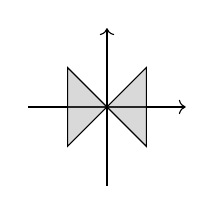
\begin{tikzpicture}
 \draw[->] (0,-1) -- (0,1);
 \draw[->] (-1,0) -- (1,0);
 \draw[fill=gray, fill opacity=0.3] (0,0) -- (0.5,-0.5) -- (0.5,0.5) -- (0,0) -- (-0.5,0.5) -- (-0.5,-0.5) -- cycle;
\end{tikzpicture}\]
\end{example}

\begin{definition}
 Let $R$ be a normed field and let $\mathbb{V}$ be a topological $R$-vector space. We say that $\mathbb{V}$ is \emph{locally convex} iff every $x\in \mathbb{V}$ admits a local basis consisting of disks at $x$.
 Since the topology of $\mathbb{V}$ is necessarily translation invariant,
 it is equivalent to only ask that $0$ has such a local basis.
\end{definition}

The main result is the following:

\begin{proposition}\label{prop:mainLCTVS}
 Let $\mathbb{V}$ be a locally convex topological $\R$-vector space (where $\R$ is endowed with its usual absolute value and the induced topology by it).
 Fix $x\in\mathbb{V}$, a neighbourhood $V\subseteq\mathbb{V}$ of $x$ and $f:V\to \R\cup\set{+\infty,-\infty}$.
 If $V$ is convex, $f$ is concave and lower bounded by a finite constant $K$, then $f$ is continuous at $x$ (w.r.t.\ the subspace topology on $V$).
\end{proposition}
\begin{proof}
 Since $V$ is a neighbourhood of $x$, $x$ admits an open neighbourhood $U\subseteq V$, and by local convexity of $\mathbb{V}$ there is a (non necessary open) disk $D\subseteq U$ at $x$.
 Now fix $\eps\in(0,1)$ and $r,s\in \R$ with $0\leq r\leq\eps$, $s=1-r$.
 Fix also $w\in D$.
 By the convexity of $D$ we have $sx+rw\in D$, and thus the convexity of $f$ entails that:
 \[
  f(sx+rw)\geq s f(x) + r f(w) \geq s f(x) + r K = (1-r)f(x) + r K
 \]
that is,
 \[
  f(x)-f(sx+rw)\leq r (f(x)-K).
 \]
 Now remark that $x=\dfrac{1}{s+2r}(sx+rw)+\dfrac{r}{s+2r}(2x-w)$, where $\dfrac{1}{s+2r}+\dfrac{r}{s+2r}=1$, $\dfrac{1}{s+2r}<1$ and $2x-w\in D$ (because $D$ is a disk at $x$).
 Therefore by the convexity of $f$ we have:
 \[
  f(x)\geq \dfrac{1}{s+2r}f(sx+rw)+\dfrac{r}{s+2r}f(2x-w)\geq \dfrac{1}{s+2r}(f(sx+rw)+rK)
 \]
 that is,
 \[
  f(sx+rw)-f(x)\leq r(f(x)-K).
 \]
 We have thus shown that $\mid f(sx+rw)-f(x)\mid\leq r(f(x)-K)$ for all $w\in D$.
 Since this holds also for all $\eps\in(0,1)$, and due to the choice of $r,s$, the points of shape $sx+rw$ span $D$ when $w$ spans $D$ and $\eps$ spans $(0,1)$.
 That is, we have shown that $\mid f(w)-f(x)\mid\leq r(f(x)-K)$ for all $w\in W$.
 Since $f(x)-K\geq 0$ and $r\leq \eps$, we have that $\exists\lim\limits_{w\to x} f(w)=f(x)$.
\end{proof}

Now we show how to apply this argument to our tropical case $\Lawv^X$, which is \emph{not} a LCTVS (because it is not a vector space).

First, we have:

\begin{corollary}\label{cor:cont}
 Let $f:({\R}_{> 0}^X,\supnorm{.}) \to (\overline\R_{\geq 0},\absv .)$ and $x\in {\R}_{> 0}^X$.
 If there is a convex neighbourhood $V\subseteq \overline{\R}_{> 0}^X$ of $x$ s.t.\ $f_{\lVert V}$ is concave, then $f$ is continuous at $x$.
\end{corollary}
\begin{proof}
 The $\R$-vector space $\R^X$ is topological w.r.t.\ the topology $\tau_\infty$ induced on it by the norm $\lVert .\lVert_\infty$, and it is clearly locally convex.
 Call $\tau^+_\infty$ the topology induced by $\supnorm{.}$ on ${\R}_{> 0}^X$.
 It is clear that it coincides with $\tau^+_\infty$.
 Since moreover ${\R}_{> 0}^X$ is open in $(\R^X,\tau_\infty)$, the neighbourhood $V$ of $x$ in $({\R}_{> 0}^X,\supnorm{.})$ is also a neighbourhood of $x$ in $(\R^X,\tau_\infty)$.
 We can therefore apply Proposition~\ref{prop:mainLCTVS} to $f_{\lVert V}$ (which is lower bounded by $0$ by definition of $f$) and obtain that $f_{\lVert V}$ is continuous at $x$ w.r.t.\ the subspace topology $\tau_V$ induced by $\tau_\infty$ on $V$.
 But since $V$ is contained in ${\R}_{> 0}^X$, the topology $\tau_V$ coincides with the subspace topology induced on $V$ by $\tau^+_\infty$.
 So $f$ is continuous at $x$ w.r.t.\ $\tau^+_\infty$.
\end{proof}

One may wonder if the same proof as above makes it possible to state the previous corollary replacing ${\R}_{> 0}^X$ with $\R_{\geq 0}^X$ (so, in particular, taking $x\in\R_{\geq 0}^X$).
This is not possible because in the proof we crucially use that $\R_{> 0}^X$ is open in $(\R^X,\tau_\infty)$, which is not the case of $\R_{\geq 0}^X$.
In fact, this allowed us to say that $V$ is a neighbourhood of $x$ in $(\R^X,\tau_\infty)$, and therefore to be able to apply Proposition~\ref{prop:mainLCTVS}.
Taking $\R_{\geq 0}^X$ instead, this is in general not true: we could have a neighbourhood of $x$ w.r.t.\ the subspace topology on $\R_{\geq 0}^X$ induced by $\tau_\infty$, which does not contain any open neighbourhood of $x$ w.r.t.\ $\tau_\infty$ (i.e. it is not a neighbourhood w.r.t.\ $\tau_\infty$).

\begin{example}
 An example of a neighbourhood of $x$ w.r.t.\ the subspace topology on $\R_{\geq 0}^X$ induced by $\tau_\infty$, which is not a neighbourhood w.r.t.\ $\tau_\infty$.
 \[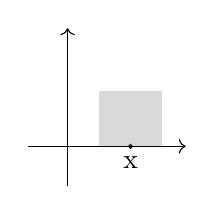
\begin{tikzpicture}
 \draw[->] (0,-0.5) -- (0,1.5);
 \draw[->] (-0.5,0) -- (1.5,0);
 \filldraw[black] (0.8,0) circle (0.7pt) node[anchor=north]{x};
 \fill[fill=gray, fill opacity=0.3] (0.4,0) -- (1.2,0) -- (1.2,0.7) -- (0.4,0.7) -- (0.4,0) -- cycle;
\end{tikzpicture}\]
\end{example}

Finally we have the desired result Theorem~\ref{thm:cont}:

\begin{theorem}[Theorem~\ref{thm:cont}]
 Tropical Laurent series $f:({\R}_{\geq 0}^X,\supnorm .) \to (\overline\R_{\geq 0},\absv .)$ are continuous on ${\R}_{> 0}^X$ w.r.t.\ the norm $\norm{\cdot}_\infty$.
\end{theorem}
\begin{proof}
 We know that tLs's are concave on all their domain.
 Therefore the result immediate follows by Corollary \ref{cor:cont}, since the topology induced by $\supnorm{.}$ on ${\R}_{> 0}^X$ coincides with the subspace topology induced by $({\R}_{\geq 0}^X,\supnorm .)$ on it.
\end{proof}

Due to the previous discussion about the impossibility of stating Corollary \ref{cor:cont} in the case where one of the coordinates of $x$ is $0$, the continuity of tLs on the hyperplanes $\mathcal H_a:=\set{x\in {\R}_{\geq 0}^X \mid x_a=0}$, for $a\in X$, must be treated separately.
Similarly, the continuity at points with infinite coordinates must be treated separately as well.
We left it for future investigations.

\begin{remark}
 We formulated the main argument (Proposition~\ref{prop:mainLCTVS}) in the general setting of LCTVS's.
We did so just to show that it is actually a general argument, but we could have placed ourselves already in a more particular setting of our interest and carry on the proof.
For instance, Theorem~\ref{thmTLSlocLip} will be proved by refining this kind of argument (Lemma~\ref{lm:mainLip}), but not in the setting of LCTVS.
\end{remark} 



%\newpage
\subsection{Section~\ref{subsec:cont}: proof of Theorem~\ref{thm:ScottCont}}

In order to prove such result we must quickly recall the theory of normed cones, which we do below.

Here we denote with $\overline{\R}_{\geq 0}$ the set $\R_{\geq 0}\cup\set{\infty}$ (the same as $\Lawv$, but we prefer to explicit it here).

\subsubsection{Normed cones}

\begin{definition}
 An \emph{$\overline{\R}_{\geq 0}$-cone} is a commutative $\overline{\R}_{\geq 0}$-semimodule with cancellative addition\footnote{I.e.: $x+y=x+y' \Rightarrow y=y'$.}.
\end{definition}

In \cite{Selinger2004} cones are required to also have ``strict addition'', meaning that $x+y=0 \Rightarrow x=y=0$.
We do not add this requirement since it will automatic hold when considering normed cones.

\begin{remark}
 The addition of a cone $P$ (which forms a commutative monoid) turns $P$ into a poset by setting:
 \[
  x \leq y \textit{ iff } y=x+z \textit{, for some }z\in P.
 \]
 By the cancellative property, when such $z$ exists it is unique, and we denote it by $y-x$.
 Such order is called the \emph{cone-order} on $P$.
\end{remark}

\begin{definition}
 A \emph{normed $\overline{\R}_{\geq 0}$-cone} is the data of a $\overline{\R}_{\geq 0}$-cone together with a $\leq$-monotone\footnote{I.e.: $x\leq y \Rightarrow \norm{x}\leq \norm y$. Remark that requiring this property (for all $x,y$) is equivalent to requiring that $\norm{x}\leq \norm{x+y}$ for all $x,y$.} norm\footnote{A \emph{norm} on a $\overline{\R}_{\geq 0}$-abstract cone $P$ is a map $\norm{.}:P\to \overline{\R}$ satisfying the usual axioms of norms:
 $\norm x \geq 0$, $\norm x = 0 \Rightarrow x=0$, $\norm{rx}=r\norm x$ and $\norm{x+y}\leq \norm x + \norm y$.} on it.
\end{definition}

In, e.g.~\cite{EhrPagTas2018}, a normed $\overline{\R}_{\geq 0}$-cone is simply called a cone.

Remark that in a normed $\overline{\R}_{\geq 0}$-cone, by monotonicity of the norm, we have: $\norm{x+y}=0 \Rightarrow x=y=0$.
Therefore, as already mentioned, in a normed cone we have: 
$x+y=0 \Rightarrow \norm{x+y}=0 \Rightarrow x=y=0$, that is, addition is strict.

\begin{example}
 $\overline{\R}_{\geq 0}^X$ is a normed cone with the norm $\supnorm{x}:=\sup\limits_{a\in X} x_a\in \overline{\R}_{\geq 0}$.
\end{example}

\begin{remark}
 The cone-order on $\overline{\R}_{\geq 0}^X$ is the pointwise usual order on $\overline{\R}_{\geq 0}$.
 
 Remark also that tLs have no reason to be linear nor sublinear.
\end{remark}

\begin{remark}\label{rmk:tropMonot}
 tLs are monotone w.r.t.\ to the cone order on its domain and codomain.
 This is clear, using the definition of tLs, because $\mu x\leq \mu y$ if $x\leq y$.
\end{remark}

\begin{remark}
 The cone-order on $\overline{\R}_{\geq 0}^X$ makes it into a dcpo with least element $0$.
\end{remark}

The following is a usual domain theoretical lemma.

\begin{lemma}\label{lm:sup=sup}
 Let $P$ be a poset and $X, I$ sets. Fix the pointwise order on $P^X$.
 \begin{enumerate}
  \item Let $x^i\in P^X$ for $i\in I$.
  If $\bigvee\limits_{i\in I} x^i$ exists $P^X$, then $\bigvee\limits_{i\in I} x^i_a$ exists in $P$ for all $a\in X$, and we have: $\bigvee\limits_{i\in I} x^i_a=\left(\bigvee\limits_{i\in I} x^i\right)_a$.
 \item Let $x^i_a\in P$ for $i\in I,a\in X$.
  If $\bigvee\limits_{i\in I} x^i_a$ exists $P$ for all $a\in X$, then $\bigvee\limits_{i\in I} x^i$ exists in $P^X$, and we have: $\left(\bigvee\limits_{i\in I} x^i\right)_a=\bigvee\limits_{i\in I} x^i_a$.
 \end{enumerate}
\end{lemma}

A \emph{directed net} in a poset $P$ with indices in a set $I$ is a function $s:I\to P$, denoted by $(s_i)_{i\in I}$, s.t.\ its image is directed.
We say that a directed net in $P$ \emph{admits a sup} iff its image admits a sup in $P$.
We say that a directed net $s$ in a normed cone is \emph{bounded} iff the set $\set{\norm{s_i}\,\mid i\in I}$ is bounded in $\R_{\geq 0}$.

Remember the definition of Scott-continuity:

\begin{definition}
 A function $f:P\to P'$ between posets is \emph{Scott-continuous} iff for all directed net $(s_i)_i$ in $P$ admitting a sup, we have $\exists \bigvee\limits_i f(s_i) = f(\bigvee\limits_i s_i)$ in $P'$. 
\end{definition}

The fundamental result in order to prove Theorem~\ref{thm:ScottCont} is the following, taken from \cite{Selinger2004}.

\begin{proposition}\label{prop:infsup}
 Let $P$ be a normed $\overline{\R}_{\geq 0}$-cone s.t.\ every bounded directed net in $P$ admits a sup.
 Let $(v_i)_{i\in I}$ be a directed net in $P$ with an upper bound $v\in P$.
 Then $\exists\bigvee\limits_{i\in I} v_i \in P$ and, if $\inf\limits_{i\in I} \norm{v-v_i} =0$, one has: $\bigvee\limits_{i\in I} v_i = v$.
\end{proposition}
\begin{proof}
 Remark that $v-v_i$ exists in $P$ by hypothesis and so does $\bigvee\limits_{i\in I} v_i$, thanks to the monotonicity of the norm.
 Now, since $v\geq v_i$ for all $i$, we have that $v\geq \bigvee\limits_{i\in I} v_i$, and so $v-\bigvee\limits_{i\in I} v_i$ exists in $P$.
 Fix $i\in I$.
 Since $v_i\leq \bigvee\limits_{i\in I} v_i$, then $v-\bigvee\limits_{i\in I} v_i\leq v-v_i$ and, by monotonicity of the norm, $\norm{v-\bigvee\limits_{i\in I} v_i}\leq \norm{v-v_i}$.
 Since this holds for all $i\in I$, we have:
 $0\leq \norm{v-\bigvee\limits_{i\in I} v_i}\leq \inf\limits_{i\in I} \norm{v-v_i}=0$, where the last equality holds by hypothesis.
 Thus $\norm{v-\bigvee\limits_{i\in I} v_i}=0$, i.e.\ $v=\bigvee\limits_{i\in I} v_i$.
\end{proof}

\begin{definition}
 A normed $\overline{\R}_{\geq 0}$-cone $P$ is \emph{Scott-complete} iff its norm is Scott-continuous (where the codomain $\overline\R_{\geq 0}$ is endowed with its usual order) and every bounded directed net in $P$ admits a sup.
 This is equivalent to asking that its closed unit ball is a dcpo.
\end{definition}

\begin{proposition}
 The normed cone $\overline{\R}_{\geq 0}^X$ is Scott-complete.
\end{proposition}
\begin{proof}
 $\overline{\R}_{\geq 0}^X$ being a dcpo, all the existences of sup's that we should check do automatically hold, so we only have to show that $\bigvee$ and $\supnorm{.}$ commute:
 $\supnorm{\bigvee\limits_i x_i}=
 \sup\limits_a\, \sup\limits_i\, (x_i)_a =
 \sup\limits_i\, \sup\limits_a\, (x_i)_a =
 \bigvee\limits_i \supnorm{x_i}$.
\end{proof}

%Let us set $\infty_b$ to be the hyper-semi-plane $\set{y\in\overline{\R}^Y_{\geq 0}\mid y_b=+\infty}$ and $\set{f<<+\infty}:=\bigcup\limits_{b\in Y} f^{-1}\infty_b$.

%\begin{remark}\label{rmk:R-f<<oo}
%Let $f:\overline{\R}^X_{\geq 0}\to\overline{\R}^Y_{\geq 0}$ be tropical.
%Then, $\R^X_{> 0}-\set{f<<+\infty}$ is a dcpo (w.r.t.\ the usual order, that is, its cone order).
%In order to see this, it is enough to show that, for any $b\in Y$ and for any directed net $(x^i)_i$ in $\R^X_{> 0}$ s.t.\ $f(x^i)_b<+\infty$ for all $i$, we have $f(\bigvee\limits_i x^i)_b<+\infty$ (where the sup is taken in $\R^X_{> 0}$).
%Such property holds because otherwise it is easy to see that $f$ would be discontinuous at the point $\bigvee\limits_i x^i\in\R^X_{> 0}$ w.r.t.\ the topology\footnote{Remark that this argument would not be possible using Scott-continuity instead. Indeed, it could well be that $f(\bigvee\limits_i x^i)_b=\bigvee\limits_i f(x^i)_b=+\infty$ while $f(x^i)_b<+\infty$ for all $i$.} induced by $\supnorm{.}$.
%This contradicts Corollary \ref{cor:tropCont}.
%\end{remark}

We finally obtain the desired:

\begin{theorem}[Theorem~\ref{thm:ScottCont}]
 All tLs $f:\overline{\R}^X_{\geq 0}\to\overline{\R}^Y_{\geq 0}$ are Scott-continuous on $\R^X_{> 0}$ w.r.t.\ the cone-orders on its domain and codomain.
\end{theorem}
\begin{proof}
 Let $(x_i)_i$ a directed net in $\R^X_{> 0}$ s.t.\ $\bigvee\limits_i x^i$ exists in $\R^X_{> 0}$.
 Then $\inf\limits_i \supnorm{\bigvee\limits_i x^i - x^i} =0$, where $\bigvee\limits_i x^i - x^i$ exists because $\bigvee\limits_i x^i \geq x^i$ for all $i$.
 Since $f$ is $\supnorm{.}$-continuous on $\R^X_{> 0}$, then $\inf\limits_i \supnorm{f(\bigvee\limits_i x^i) - f(x^i)} =0$, where $f(\bigvee\limits_i x^i) - f(x^i)$ exists because $f(\bigvee\limits_i x^i) \geq f(x^i)$ for all $i$ being $f$ monotone (Remark \ref{rmk:tropMonot}).
 We can therefore apply Proposition \ref{prop:infsup} to the directed net $(f(x^i))_i$ in $\overline{\R}^Y_{\geq 0}$, obtaining that $\bigvee\limits_i f(x^i)$ exists in $\overline{\R}^Y_{\geq 0}$ and it coincides with $f(\bigvee\limits_i x^i)$.
\end{proof}

%\begin{remark}
%By looking at the definition of tropical functions, for $f$ tropical we have that: if $x,x'\in\R^X_{> 0}-\set{f<<+\infty}$ and $r\in\R_{> 0}$, then $x+x',rx\in\R^X_{> 0}-\set{f<<+\infty}$.
%That is, $\R^X_{> 0}-\set{f<<+\infty}$ is a $\R_{>0}$-cone.
%It is clearly still Scott-complete.
%\end{remark}

In the main paper we mention that $\R_{\geq0}^X$ is a Scott-complete dcpo.
We did not state it as a theorem because it follows from standard and well-known domain theoretical considerations.
Let us prove it here anyway.

Recall the definition of Scott-complete dcpo:

\begin{definition}
 Let $P$ be a dcpo and define a relation by: $x<<y$ iff for all directed $D\subseteq P$, if $y\leq \bigvee D$, then $x\leq d$, for some $d\in D$.
 Call $\twoheaddownarrow y:=\set{x\in P\mid x<<y}$.
 A dcpo $P$ is \emph{Scott-continuous} iff $\twoheaddownarrow x$ is directed and $x=\bigvee\twoheaddownarrow x$ for all $x\in P$.
\end{definition}

\begin{remark}
 In any dcpo we have: $\twoheaddownarrow x \subseteq \downarrow x$.
 This immediately follows by considering the directed set $\set{x}$.
\end{remark}

\begin{lemma}\label{lm:<<dir}
 In $\overline{\R}_{\geq 0}^X$, every set $\twoheaddownarrow x$ is directed.
\end{lemma}
\begin{proof}
 It is immediate that $0\in\twoheaddownarrow x$, so it is non-empty.
 Now let $y,y' << x$.
 Since we are in $\overline{\R}_{\geq 0}^X$, there is $y\vee y'\in\overline{\R}_{\geq 0}^X$.
 So we only have to show that $y\vee y'<<x$.
 For that, let $D$ be a directed set in $\overline{\R}_{\geq 0}^X$ s.t.\ $x\leq\bigvee D$.
 Since $y,y' << x$ we find $d,d'\in D$ s.t.\ $y\leq d$, $y'\leq d'$.
 Since $D$ is directed, there is $\hat d\in D$ s.t.\ $y\leq d\leq \hat d\geq d'\geq y'$.
 But then, by definition of sup, it must be $\hat d\geq y\vee y'$ and we are done.
\end{proof}

\begin{remark}
 The following is a known property (that we will not use):
 let $P$ be a complete normed cone which is a dcpo w.r.t.\ its cone-order. Then $P$ is Scott-continuous as a dcpo iff its closed unit ball is Scott-continuous as a dcpo.
\end{remark}

\begin{remark}\label{rmk:<<R}
 Consider $\overline{\R}_{\geq 0}$ with its usual order (which coincides with its cone-order).
 It is easily seen (and well known) that $y<<x$ iff either $y=0$ or $y<x$.
 This immediately implies that $\overline{\R}_{\geq 0}$ is Scott-continuous, since $x=\sup\limits_{y<x} y$.
\end{remark}

\begin{lemma}\label{lm:<<RX}
 Let $x,y\in \overline{\R}_{\geq 0}^X$ (considered as a dcpo with its cone order, which is the pointwise one). Fix $a\in X$.
 If $y_a<<x_a$ and $y_c=0$ for all $c\neq a$, then $y<<x$.
\end{lemma}
\begin{proof}
 Towards a contradiction, assume that there is a directed set $D$ in $\overline{\R}_{\geq 0}^X$ with $x\leq\bigvee D$ and s.t.\ $y\not\leq d$ for all $d\in D$.
 Call $D_a:=\set{d_a\mid d\in D}$ and remark that it is directed, because $D$ is.
 Also, by Lemma \ref{lm:sup=sup}, $\bigvee D_a = \left(\bigvee D\right)_a$.
 Therefore from $y_a<<x_a\leq \bigvee D_a$ we obtain a $d\in D$ s.t.\ $y_a\leq d_a$.
 By the absurd hypothesis we have $y\not\leq d$, so there must be $c\in X$ s.t.\ $y_c\not\leq d_c$, i.e. (because real numbers are totally ordered) $y_c>d_c$.
 Therefore it must be $c\neq a$.
 But then we have $0=y_c>d_c\geq 0$, contradiction.
\end{proof}

\begin{lemma}\label{lm:<<_a}
 In $\overline{\R}_{\geq 0}^X$ we have:
 if $y<<x$ then $y_a<< x_a$ for all $a\in X$.
\end{lemma}
\begin{proof}
 Fix $a\in X$.
 Let $D$ directed set in $\overline{\R}_{\geq 0}$ s.t.\ $x_a\leq\bigvee D$.
 We look for a $d\in D$ s.t.\ $y_a\leq d$.
 For $d\in D$, let $x^{a,d}\in\overline{\R}_{\geq 0}^X$ defined by $x^{a,d}_c:=x_c$ if $c\neq a$ and $x^{a,d}_a:=d$.
 Let $D^x_a:=\set{x^{a,d}\mid d\in D}$.
 By Lemma \ref{lm:sup=sup} $D^x_a$ admits sup in $\overline{\R}_{\geq 0}^X$ and it is $(\bigvee D^x_a)_c=x_c$ if $c\neq a$ and $(\bigvee D^x_a)_a=\bigvee D$.
 Hence, $x\leq \bigvee D^x_a$.
 If we prove that $D^x_a$ is directed, we are done: indeed, since $y<<x$, there is $d\in D$ s.t.\ $y\leq x^{a,d}$ and thus, in particular, $y_a\leq x^{a,d}_a=d$.
 Let us finally prove that $D^x_a$ is directed: it is clearly non-empty, since $D$ is.
 Let now $d,d'\in D$.
 We want to show that there is $\hat d\in D$ s.t.\ $x^{a,d}\leq x^{a,\hat d}\geq x^{a,d'}$.
 But since $D$ is directed, there is $\hat d\in D$ s.t.\ $d\leq \hat d\geq d'$, and therefore $x^{a,d}_c=x_c= x^{a,\hat d}_c =x_c=x^{a,d'}_c$ for all $c\neq a$, and $x^{a,d}_a=d\leq \hat d=x^{a,\hat d}_a=\hat d \geq d'=x^{a,d'}_a$.
\end{proof}

\begin{lemma}\label{rmk:sup_a=sup_a}
In $\overline{\R}_{\geq 0}^X$ we have:
$\bigvee\limits_{y<<x_a} y = \bigvee\limits_{y<<x} y_a$.
\end{lemma}
\begin{proof}
 If we show that $\twoheaddownarrow x_a = \set{y_a\mid y\in\twoheaddownarrow x}$, then we are done because in the statement we are taking their sup's.
 The inclusion ($\supseteq$) immediately follows from Lemma \ref{lm:<<_a}. For ($\subseteq$), let $d<< x_a$.
 Then the $y\in \overline{\R}_{\geq 0}^X$ defined by $y_c:=0$ if $c\neq a$ and $y_a:=d$, is s.t.\ $y\in\twoheaddownarrow x$ by Lemma \ref{lm:<<RX}.
 Thus, $d\in \set{y_a\mid y\in\twoheaddownarrow x}$.
\end{proof}


\begin{corollary}
 The dcpo $\overline{\R}_{\geq 0}^X$ is Scott-continuous.
\end{corollary}
\begin{proof}
 The fact that $\twoheaddownarrow x$ is directed is given by Lemma \ref{lm:<<dir}. The fact that $x=\bigvee \twoheaddownarrow x$ is given by the following equalities:
 $x_a=\bigvee\limits_{y<<x_a} y = \bigvee\limits_{y<<x} y_a = \left(\bigvee\limits_{y<<x} y\right)_a=\left(\bigvee \twoheaddownarrow x\right)_a$.
 The first equality follows from Remark \ref{rmk:<<R}, the second one from Lemma \ref{rmk:sup_a=sup_a}, the third one from Lemma \ref{lm:sup=sup}.
\end{proof}

%\newpage



\subsection{Proofs from Section~\ref{sec:4C}}


\subsubsection{Lipschitz continuity}


  We need a first, preliminary, lemma:
\begin{lemma}\label{lemma:inf}
Let $u,v: I\to Q$ and suppose $|u(i)-v(i)|\leq \delta$, for all $i\in I$.
Then $|\inf_{i\in I}u(i)- \inf_{i\in I}v(i)|\leq \delta$. 
\end{lemma}
\begin{proof}
Let $A=\inf_{i\in I}u(i)$ and $B=\inf_{i\in I}v(i)$ and suppose $A\geq B$. 
Suppose by way of contradiction $|A-B|> \delta$; then there exists $i\in I$ such that 
$v(i)<A$ and $|A-v(i)|> \delta$. Indeed, otherwise we would have $|A-B|= \sup\{ |A-v(i)|\mid v(i)\leq A\}\leq \delta$. 
Now, from $|A-v(i)|> \delta$ and $v(i)< A$ we deduce that $|u(j)-v(i)|> \delta$ for all $j\in I$, and thus in particular that $|u(i)-v(i)|>\delta$, against the assumption. We conclude then $|A-B| \leq \delta$.
In case $B\geq A$, we can argue in a similar way. 
\end{proof}



\begin{proposition}\label{prop:troplinear}
All tropical linear functions $f: \Lawv^{X}\to \Lawv^{Y}$ are non-expansive.  
\end{proposition}
\begin{proof}
%All functions of the form $f_{\theta,\eta}(x)_{b}= \theta(b)+x_{\eta(b)}$, where $\theta:Y \to \Lawv$ and $\eta:Y\to X$, are non-expansive: indeed $|f_{\theta,\eta}(x)_{b}-f_{\theta,\eta}(y)_{b}|= |\theta(b)+x_{\eta(b)}-\theta(b)-y_{\eta(b)}|=
%|x_{\eta(b)}-y_{\eta(b)}|\leq \norm{x-y}_{\infty}$.
Let $f(x)_{b}=\inf_{a}\{\widehat f_{a,b}+x_{a}\}$.
For all $a\in X$ we have that 
$|(\widehat f_{a,b}+x_{a})- (\widehat f_{a,b}+y_{a})|=
|x_{a}-y_{a}|\leq \norm{x-y}_{\infty}$. Using Lemma \ref{lemma:inf}, we deduce then 
$|f(x)_{b}-f(y)_{b}|=|\inf_{a}\{\widehat f_{a,b}+x_{a}\}-
\inf_{a}\{\widehat f_{a,b}+y_{a}\}|\leq \norm{x-y}_{\infty}$.
\end{proof}






\begin{lemma}\label{lm:mainLip}
Let $f: [0,\infty)^{X}\to Q$ be concave, monotone increasing, and continuous.  
Let $ x \neq  y  \in [0,\infty)^{X}$, with $\| x - y  \|_{\infty}<\infty$, and let $S( x ,  y  )=\{ \alpha x  + (1-\alpha) y  \mid \alpha \in [0,1]\}$ be the segment generated by $ x $ and $ y  $. 
Then $f$ is Lipschitz-continuous over $S( x ,  y  )$.

\end{lemma}
\begin{proof}
Let us prove the lemma under the assumption that for all $a\in X$, $ y  _{a}- x _{a}\geq 1$. From the fact that the claim holds under the assumption, we can deduce the claim of the lemma:
indeed for $\alpha\in (0,1)$ large enough we have that $ y  ':= \frac{ y  -\alpha x }{1-\alpha}$ is such that $ y  \in S( x ,  y  ')$ (and thus $S( x ,  y  )\subseteq S( x ,  y  ')$) and 
$ y  '_{a}- x _{a}\geq 1$. Hence from our proof we deduce that $f$ is Lipschitz-continuous over $S( x ,  y  ')$, and thus a fortiori over $S( x ,  y  )$ too.


Since $f$ is continuous over $[0,\infty)^{X}$ and $S( x ,  y  )$ is compact, $f$ admits a maximum $\mathrm{MAX}$ over $S( x ,  y  )$.
For all $ z  <  z  '\in S( x ,  y  )$, let $M( z  ,  z  ')\in Q^{X}$ be defined by
$$
M( z  ,  z  ')_{a}= \frac{f( z  ')-f( z  )}{ z  '_{a}- z  _{a}}
$$
Observe that
\begin{align*}
M( x ,  y  )_{a} & = \frac{f( y  )-f( x )}{ y  _{a}- x _{a}} \leq 
f( y  )-f( x ) \leq \mathrm{MAX}
\end{align*}
using the fact that $ y  _{a}- x _{a}\geq 1$. 

We now claim that $M( z  ,  z  ')$ is contravariant in both $ z  $ and $ z  '$. 
Indeed suppose $ z  \leq  z  '' <  z  '$, so that $ z  = \lambda  z  ' +(1-\lambda) z  ''$ for some $\lambda \in (0,1)$. Then, using the fact that $f$ is concave, we have 
\begin{align*}
M( z  ,  z  ')_{a}&=\frac{f( z  ')-f(\lambda  x  +(1-\lambda) z  '')}{ z  '_{a}-\lambda  x _{a} -(1-\lambda) z  ''_{a}} \\
&
\geq 
\frac{f( z  ')-\lambda f( z  ') -(1-\lambda)f( z  '')}{ z  '_{a}-\lambda  z  '_{a} -(1-\lambda) z  ''_{a}} \\
&
= 
\frac{(1-\lambda)(f( z  ')-f( z  ''))}{(1-\lambda ) z  '_{a}- z  ''_{a}} =M( z  '',  z  ')
\end{align*}
In a similar way it is shown that for $ z   <  z  ''\leq  z  '$, $M( z  , z  ')\leq M( z  ,  z  '')$. 

Therefore, for all $ z   <  z  '\in S( x ,  y  )$, we have that $M( z  ,  z  ')_{a} \leq M( x ,  z  ')_{a} \leq M( x ,  y  )_{a} \leq \mathrm{MAX}$. 
From this, using the fact that $f$ is monotone increasing, we deduce that 
$|f( z  ')-f( z  )|=f( z  ')-f( z  ) \leq \mathrm{MAX}\cdot | z  '_{a}- z  _{a}|
$ and thus that 
$$|f( z  ')-f( z  )|\leq \mathrm{MAX}\cdot \| z  '- z  \|_{\infty}$$
that is, that $f$ is $\mathrm{MAX}$-Lipschitz over $S( x ,  y  )$. 
\end{proof}

\begin{proposition}
Let $f: [0,\infty)^{X}\to Q$ be concave, monotone increasing, and continuous.  
For all $\epsilon \in (0,\infty)$ and $ x \in [0,\infty)^{X}$, $f$ is Lipschitz-continuous over the open ball $B( x , \epsilon)$.
\end{proposition}
\begin{proof}
Let $\mathrm{MAX}$ indicate the maximum of $f$ over $B( x , \epsilon)$. 
Let $ y  ,  z  \in B( x , \epsilon)$; then $\| y  - z  \|_{\infty}\leq 2\epsilon < \infty$, so by the lemma above $f$ is $K$-Lipschitz over the segment $S( y  ,  z  )$ for some $K\leq \mathrm{MAX}$, so we deduce $|f( y  )-f( z  )|\leq \mathrm{MAX}\cdot \| y  - z  \|_{\infty}$.
\end{proof}

\begin{theorem}[local Lipschitz-continuity]
Let $f: [0,\infty)^{X}\to Q$ be concave, monotone increasing, and continuous.  
Then $f$ is locally Lipschitz-continuous.
\end{theorem}
\begin{proof}
For all $ x \in [0,\infty)^{X}$, $f$ is Lipschitz-continuous over the open set $B( x , 1)$.
\end{proof}



\subsubsection{Characterizations of the functional metric }



  \begin{proposition}\label{prop:functionalmetric}
For all maps $f,g: Q\langle X\rangle\to Q\langle Y\rangle$,  
$$
  \|\widehat f- \widehat g\|_{\infty}=
  \sup\{\|f( x )- g( x )\|_{\infty} \mid  x \in Q\langle X\rangle\}
$$

\end{proposition}
  
%
%\begin{lemma}
%Let $f,g\in\mathsf{Trop}(1,1)$ (i.e.~$f,g:Q\to Q$), and suppose for all $n\in \BB N$, 
%$|\widehat f_{n}-\widehat g_{n}|\leq \delta$. Then for all $x\in Q$, $|f(x)-g(x)|\leq \delta$.
%
%\end{lemma}
%\begin{proof}
%$|f(x)-g(x)|= |( \inf_{n}nx+\widehat f_{n})- (\inf_{n}nx+\widehat g_{n})|$. 
%Since $|nx+\widehat f_{n} - nx -\widehat g_{n}|= |\widehat f_{n}-\widehat g_{n}|\leq \delta$, by the Lemma above we conclude $|f(x)-g(x)|\leq \delta$. 
%\end{proof}



  
  \begin{proof}[Proof of Proposition \ref{prop:functionalmetric}]
For one side, suppose for all $\mu\in \C  M_{\mathrm{fin}}(X),b\in Y$, 
$|\widehat f_{\mu,b}-\widehat g_{\mu,b}|\leq \delta$. Then for all $ x \in Q\langle X\rangle$ and $b\in Y$, $|f( x )(b)-g( x )(b)|\leq \delta$.
Indeed, $|f( x )(b)-g( x )(b)|= |( \inf_{\mu}\mu  x +\widehat f_{\mu,b})- (\inf_{\mu}\mu  x +\widehat g_{\mu,b})|$. 
Since $|\mu  x +\widehat f_{\mu,b} - \mu  x  -\widehat g_{\mu,b}|= |\widehat f_{\mu,b}-\widehat g_{\mu,b}|\leq \delta$, by Lemma \ref{lemma:inf} we conclude $|f( x )(b)-g( x )(b)|\leq \delta$. 


For the other side, suppose for some $\mu\in \C M_{\mathrm f}(X)$ and $b\in Y$, $|\widehat f_{\mu,b}-\widehat g_{\mu,b}|> \epsilon$; 
then, by letting $e_{\mu}\in Q\langle !X\rangle$ be the (tropical) characteristic function of $\mu$, we have
 $|f(e_{\mu})({b})-g(e_{\mu})({b})| =
|( \inf_{\mu'}\widehat f_{\mu',b}+ \mu'(e_{\mu}))-
( \inf_{\mu'}\widehat g_{\mu',b}+\mu'(e_{\mu}))|=
|\widehat f_{\mu,b}- \widehat g_{\mu,b}|> \epsilon$, so we deduce that 
$\sup\{\| f( x )- g( x ) \|_{\infty}\mid  x \in Q\langle X\rangle\}> \epsilon$.
\end{proof}


The second characterization relates distances with the Taylor expansion. Let us briefly discuss the latter, first.
For all $f: Q\langle X\rangle \to Q\langle Y\rangle$, let $\delta^{(n)}f:Q\langle X^{n}\rangle \to Q\langle Y\rangle$ indicate the $n$-linear function given by 
$$
\delta^{(n)}f( x ^{n})= D^{(n)}f( x ^{n}, \infty)
$$

Notice that $\widehat{\delta^{(n)}f}\in Q^{X^{n}\times Y}$ satisfies 
$\widehat{\delta^{(n)}f}_{a_{1},\dots, a_{n},b}= \widehat f_{[a_{1},\dots, a_{n}],b}$.
In other words, $\delta^{(n)}f$ precisely captures the behavior of $f$ when applied to multisets of length $n$. Moreover, the full behavior of $f$ can be recovered from the functions $\delta^{(n)}f$ using the Taylor expansion which, in its tropical form, reads as:
\begin{equation*}
f( x )= \inf_{n}\left \{ D^{(n)}f( x ^{n},\infty)\right\}= \inf_{n}\left \{\delta^{(n)}f( x ^{n})\right\}
%\tag{Tropical Taylor}
\end{equation*}





\begin{proposition}\label{prop:taylormetric}
For all $f,g:Q\langle X\rangle \to Q\langle Y\rangle$, 
$$
\| \widehat f-\widehat g\|_{\infty}= \sup_{n}\| \widehat{\delta^{(n)}f} -\widehat{\delta^{(n)}g}\|_{\infty}
$$
\end{proposition}
\begin{proof}
Let us first show that $\| \widehat f-\widehat g\|_{\infty}\leq \epsilon$ implies 
$\| \delta^{(n)}f-\delta^{(n)}g\|_{\infty}\leq\epsilon$, for all $n\in \BB N$. 
Notice that $\widehat{\delta^{(n)}f}\in Q^{X^{n}\times Y}$ satisfies 
$\widehat{\delta^{(n)}f}_{a_{1},\dots, a_{n},b}= \widehat f_{[a_{1},\dots, a_{n}],b}$. Hence 
from $\| \widehat f-\widehat g\|\leq\epsilon$ it follows that for all $\mu=[a_{1},\dots, a_{n}]$ and $b\in Y$, 
$|\widehat f_{\mu,b}- \widehat g_{\mu,b}|\leq \epsilon$, so 
we deduce that $\| \widehat{\delta^{(n)}f}- \widehat{\delta^{(n)}g}\|\leq \epsilon$.

For the converse direction suppose that, for all $n\in \BB N$, $\| \widehat{\delta^{(n)}f}- \widehat{\delta^{(n)}g}\|\leq \epsilon_{n}$. Then, since the family of coefficients $
F_{n,\mu,b}=
( \widehat{\delta^{(n)}f})_{a_{1},\dots, a_{n},b}$ (where $\mu=[a_{1},\dots, a_{n}]$) is in bijection with the coefficients $\widehat f_{\mu,b}$, we deduce that $|\widehat f_{\mu,b}-\widehat g_{\mu,b}|\leq 
\epsilon_{\sharp \mu  }$, and thus that 
$\| \widehat f-\widehat g\|_{\infty}\leq \sup_{n}\epsilon_{n}$. 
\end{proof}



\newpage
\section{Proofs from Section VII}


In the following we let $Q$ indicate the Lawvere quantale $([0,\infty], \geq, +,0)$. 
$Q$ can be seen as:
\begin{itemize}
\item a category $Q_{0}$ with a unique object and morphisms being the elements of $Q$, with identity 0 and composition $+$;

\item a degenerate category $Q_{1}$ with objects the elements of $Q$, and  
a morphism between $x$ and $y$ whenever $x\geq y$;

\item a 2-category $Q_{2}$ with 0-cells and 1-cells as in $Q_{0}$, and 2-cells the morphisms of $Q_{1}$.

\end{itemize}
These categorical formulations of $Q$ will help us here and there. 

We let $x-y$ indicate truncated subtraction. Notice that 
$x \leq (x-y)+y$ and $(x+y)-y\leq x$. This corresponds to the fact that ``$\_-y$'', as a functor from $
Q_{1}$ to itself, 
 is \emph{right-adjoint} to the functor ``$\_+y$''. Equivalently, 
 $x+y \geq z $ iff $x\geq z-y$.




$Q\mathsf{Rel}$ is the category of sets and $Q$-relations, where a $Q$-relation 
$R:X\pfun Y$ is a function $R: X\times Y\to Q$, with identity $1_{X}:X\pfun X$ given by 
$$1_{X}(x,y)=\begin{cases} 0 & \text{ if }x=y\\ \infty & \text{ otherwise}\end{cases}$$
and composition of $R:X\pfun Y$ and $S:Y\pfun Z$ given by 
$$
(S\cdot R)(x,z)= \inf_{y\in Y}R(x,y)+S(y,z)
$$ 

\begin{remark}
$Q\mathsf{Rel}$ is also a (degenerate) 2-category, where for $R,S:X\pfun Y$, $R\To S$ iff for all $x\in X$, $y\in Y$, $R(x,y)\geq S(x,y)$. 

\end{remark}


Composition with $R:X\pfun Y$ in Q$\mathsf{Rel}$ yields a functor
$$
R\cdot \_ : Q\mathsf{Rel}(A,X)   \longrightarrow Q\mathsf{Rel}(A,Y)
$$
which
has a right-adjoint
$$
\_ \multimapinv R : Q\mathsf{Rel}(A,Y)   \longrightarrow Q\mathsf{Rel}(A,X)
$$
given, for $S:A\pfun Y$ by 
\begin{align*}
(S\multimapinv R)(a,x)= \sup_{y\in Y}S(a,y) -R(x,y)
%(R\multimap S)(a,x)= \sup_{y\in Y}
\end{align*}

%
%\begin{lemma}
%\begin{itemize}
%\item[i.] $ (R\multimapinv T)\cdot
%(T\multimapinv S)\leq R \multimapinv S $.
%
%\item[ii.] $R\multimapinv T \leq (R\multimapinv S)\multimapinv (T\multimapinv S)$.
%\end{itemize}
%\end{lemma}
%\begin{proof}
%\begin{align*}
%(R\multimapinv S)(x,y)&= \sup_{z}R(x,z)-S(y,z) \\
%&=\sup_{z} (R(x,z)-T(z,z))+(T(z,z)-S(y,z))\\
%&= \inf_{w}\left(\sup_{z}R(x,z)-T(w,z)\right) +\left(\sup_{z'}T(w,z')-S(z',y)\right)
%\\
%&= \inf_{w}(R\multimapinv T)(x,w)+(T\multimapinv S)(w,y)  
%\\
%&= (R\multimapinv T)\cdot (T\multimapinv S)(x,y)
%\end{align*}
%
%\end{proof}

\subsubsection{$Q$-categories.}


A \emph{$Q$-category}, or \emph{generalized (quasi-)metric space} is a small $Q$-enriched category. Concretely, it is given by a pair $(X,q)$ made of a set $X$ and a $Q$-relation $q: X\pfun X$ satisfying:
\begin{align}
q(x,x) & = 0 \tag{Q1} \\
q(x,z)+q(z,y) & \geq q(x,y) \tag{Q2}
\end{align}
A $Q$-category is \emph{skeletal} if it further satisfies
\begin{align}
q(x,y) & = 0 \ \To \ x=y \tag{Q3}
 \end{align}
 and \emph{symmetric} if it satisfies
 \begin{align}
q(x,y) & = q(y,x) \tag{Q4}
 \end{align}
For simplicity, in the following we indicate the distance function of a $Q$-category $X$ simply as $X(x,y)$. 

\begin{remark}
In more abstract terms, a $Q$-category can be identified with a \emph{monad} in $Q\mathsf{Rel}$, seen as a 2-category: it is given by a 1-cell $q:X\pfun X$ together with 2-cells $1_{X}\To  q$ and $q\cdot q \To q$. 
\end{remark}


We let $x\simeq y$ indicate the equivalence relation defined by  $X(x,y)=X(x',y)$ holds for all $y\in X$. 
Notice that $x\simeq y$ coincides with $x=y$ precisely when $X$ is skeletal.

Every $Q$-category $X$ is also a preorder $(X,\preceq_{X})$, with $x\preceq_{X}y$ iff $X(x,y)=0$. Moreover, if $X$ is skeletal, then $\preceq_{X}$ is an order.

For every $Q$-category $X$, the category $X^{\mathrm{op}}$ has same objects as $X$, and $X^{\mathrm{op}}(x,y)=X(y,x)$. 



\begin{example}
$Q$ is a $Q$-category with the distance $Q(x,y)=y-x$. 
The category $Q^{\mathrm{op}}$ has distance $Q^{\mathrm{op}}(x,y)=Q(y,x)$.
\end{example}

\begin{example}
For every $Q$-category $X$, the distance $\C S(X)(x,y)=\max\{X(x,y),X^{\mathrm{op}}(x,y)\}$ defines a symmetric $Q$-category $\C S(X)$. In the case of $Q$, $\C S(Q)$ is just the Euclidean distance.
\end{example}






A \emph{functor} between $Q$-categories $X$ and $Y$ is just a non-expansive function $f:X\to Y$, that is, satisfying $Y(f(x),f(y))\leq X(x,y)$.

%
\begin{remark}\label{rem:functor}
Given $f:X\to Q$, $f$ is a functor precisely when for all $x,y\in X$ $f(x)\leq\inf_{x'\in X}f(x')+X(x',x)$. 
Indeed, if $f$ is a functor then $f(x)\leq f(x')+X(x',x)$, since $f(x)-f(x')=Q(f(x'),f(x))\leq X(x',x)$. 
Conversely, if $f(x)\leq f(x')+X(x',x)$ holds for all $x'$, then 
$Q(f(x),f(x'))=f(x')-f(x)\leq X(x',x)$. 
\end{remark}

%Indeed, being a functor means that any arrow $X(x,y)$ is mapped into an arrow $Y(f(x),f(y))$, that is, $Y(f(x),f(y))

\begin{example}
For every $Q$-category $X$, the $Q$-category $[X,Q]$ has objects all functors from $X$ to $Q$ (where the latter is seen as a $Q$-category), and $[X,Q](f,g)=\sup_{x\in X}Q(f(x),g(x))$.

When $X$ has the discrete metric, $[X,Q]=Q^{X}$ and $\C S([X,Q])(f,g)=\| f-g\|_{\infty}$.

 
\end{example}


\begin{example}
For every $Q$-categories $X,Y$ we can define:
\begin{itemize}
\item a $Q$-category $X\otimes Y$ with 
$(X\otimes Y)(\langle x,y\rangle, \langle x',y'\rangle)=X(x,x')+Y(y,y')$;
\item a $Q$-category $X\times Y$ with 
$(X\times Y)(\langle x,y\rangle, \langle x',y'\rangle)=\max\{X(x,x'),Y(y,y')\}$. 
\end{itemize}
\end{example}

\subsubsection{$Q$-distributors.}

%We let $Q\mathsf{Cont}$ indicate the category of $Q$-categories and continuous functors. 

A \emph{$Q$-distributor} $\Phi: X\pfun Y$ is a $Q$-relation $\Phi: X\times Y\to Q$ satisfying
\begin{align*}
\Phi\cdot X   \leq\Phi \qquad \qquad
Y \cdot \Phi  \leq \Phi
\end{align*}

\begin{remark}
Using Remark \ref{rem:functor}, it follows that $\Phi$ is a $Q$-distributor precisely when it is a functor $\Phi: X^{\mathrm{op}}\otimes Y \to Q$:
the condition $\Phi(x,y) \leq X(x,x')+\Phi(x',y)$ implies that $\Phi$ is a functor over $X^{\mathrm{op}}$, while
the condition $\Phi(x,y) \leq \Phi(x,x')+Y(x',y)$ implies that $\Phi$ is a functor over $Y$.
But this implies then 
$\Phi(x,y) \leq X(x,x') +\Phi(x',y')+Y(y',y)$ and thus $Q(\Phi(x',y'),\Phi(x,y))\leq X(x,x')+Y(y',y)$.
\end{remark}


%where $(\Phi\cdot X)_{x,y}= \inf_{z\in X}\Phi_{x,z}+X(z,y)$ and 
%$(y\cdot \Phi)_{x,y}= \inf_{z\in X}Y(x,z)+\Phi_{z,y}$.

The identity distributor $1_{X}:X\pfun X$ is given by $(1_{X})_{x,y}=X(x,y)$. 
Distributors $\Phi:X\pfun Y$ and $\Psi:Y\pfun Z$ compose via $\Psi\cdot \Phi:X\pfun Z$. 
We let $Q\mathsf{Dist}$ indicate the category of $Q$-categories and $Q$-distributors. 

\begin{remark}
Usually distributors $\Phi: X\pfun Y$ are presented as $Q$-relations $\Phi:Y\times X\to Q$ (notice the inversion of $X$ and $Y$), that is, as functors $\Phi: X\times Y^{\mathrm{op}}\to Q$. We chose to invert the presentation of distributors for uniformity with the usual notations in models of the differential $\lambda$-calculus. 
\end{remark}

Any functor $f:X\to Y$ induces two adjoint distributors $f^{\circ}:X\pfun Y$ and $f_{\circ}:Y\pfun X$ given by $f^{\circ}(x,y)=Y(f(x),y)$ and $f_{\circ}(y,x)=Y(f(y),x)$.
Here adjoint means that $1_{X}\leq f_{\circ}\cdot f^{\circ} $ and $f^{\circ}\cdot f_{\circ}\geq 1_{Y}$. 



\begin{remark}[Yoneda embedding]
%$Q$ is a $Q$-category with $Q(x,y)=|x-y|$. 
%For any $Q$-category $X$ we can define a new $Q$-category $\mathsf{Dist}(X,Q)$ (that we note simply as $[X,Q]$) whose objects are the distributors $\B x:\B 1\pfun X$, or equivalently, the functors from $X$ to $Q$, i.e.~those $\B x\in Q^{X}$ such that $|\B x_{a}-\B x_{b}|\leq X(a,b)$, or equivalently $\B x_{a}+X(a,b) \geq \B x_{b}$.


The \emph{Yoneda embedding} is the faithful functor $\C Y: X\to [X,Q]$ given by $\C Y(x)(y)=X(y,x)$. The functoriality and faithfulness of $\C Y$ follow from
\begin{align}
[X,Q](\C Y(x),\C Y(x'))= X(x,x') \tag{Yoneda}
\end{align}
which is proved as follows: for all $y\in X$ we have 
\begin{align*}
Q( \C Y(x)(y),\C Y(x')(y))&= \C Y(x')(y)-\C Y(x)(y) \\
&= X(y,x')-X(y,x) \leq X(x,x')
\end{align*}
where the last step follows from $X(y,x)+X(x,x')\geq X(y,x')$. 
From this we deduce that $[X,Q](\C Y(x),\C Y(x'))=\sup_{y\in X}Q( \C Y(x)(y),\C Y(x')(y))\leq X(x,x')$. 
For the converse direction, we have  
\begin{align*}
X(x,x') &  = X(x,x') - 0 \\ &=
X(x,x')- X(x,x)
\\& =\C Y(x')(x)-\C Y(x)(x)= Q(\C Y(x)(x),\C Y(x')(x))\\
&\leq [X,Q](\C Y(x), \C Y(x'))
\end{align*}
\end{remark}


\begin{remark}
The \emph{opposite Yoneda embedding} is the faithful functor
$\C Y^{\mathrm{op}}: X\to [X,Q]^{\mathrm{op}}$ given by $\C Y^{\mathrm{op}}(x)(y)=X(x,y)$. The functoriality and faithfulness of $\C Y^{\mathrm{op}}$ follow from
\begin{align}\label{eq:yonedaop}
[X,Q](\C Y^{\mathrm{op}}(x),\C Y^{\mathrm{op}}(x'))= X(x',x) \tag{Yoneda$^{\mathrm{op}}$}
\end{align}
which is proved similarly to the case of $\C Y$.
\end{remark}

\subsubsection{cocompleteness}



Let $\Phi:Y\pfun Z$ be a distributor and $f:Y\to X$ be a functor.
A functor $ g:Z\to X$ is called the \emph{$\Phi$-weighted colimit of $f$} if it satisfies, for all
$z\in Z$ and 
 $x\in X$, 
$$
X(g(z), x) \ = \  \sup_{y\in Y}X(f(y),x) - \Phi(y,z)
$$
If this colimit exists, we write it as $\mathrm{colim}(\Phi,f)$.


A $Q$-category $X$ is said \emph{cocomplete} if it admits all weighted colimits, and a functor $f:X\to Y$ of $Q$-categories is said \emph{cocontinuous} if it commutes with all weighted colimits, meaning that $f \circ \mathrm{colim}(\Phi,g)= \mathrm{colim}(\Phi, f\circ g)$.



We let $Q\mathsf{CCat}$ indicate the category of skeletal and cocomplete $Q$-categories and cocontinuous functors. 



\begin{proposition}\label{prop:yonedasup}
Let $X$ be a $Q$-category. Then $X$ is cocomplete iff the Yoneda embedding has a left-adjoint.
\end{proposition}
\begin{proof}
 For all $\B x\in [X,Q]$, let $\sup\B x$ be defined as a weighted colimit via
$$
X(\sup\B x, y)= \sup_{z\in X} X(z,y)-\B x_{z}
$$
that is, $\sup \B x= \mathrm{colim}( \B x, \mathrm{id}_{X})$, where $\B x$ is seen as a distributor $\B x:\B 1\pfun X$.


Let us check that $\sup: [X,Q]\to X$ is a functor. First, let us check the  inequality
\begin{align}\label{eq:in1}
(X\multimapinv\B y)\cdot (\B y\multimapinv\B x)\geq (X\multimapinv\B x)\end{align}
as follows:
\begin{align*}
\left((X\multimapinv \B y)\cdot (\B y\multimapinv\B x)\right)(a)&=
 \left (\sup_{b}X(b,a)-\B y_{b}\right)+\left(\sup_{b}\B y_{b}-\B x_{b}\right)\\
&\geq
\sup_{b}(X(b,a)-\B y_{b})+(\B y_{b}-\B x_{b})
\\
&=\sup_{b}(X(b,a)-\B y_{b}+\B y_{b})-\B x_{b}
\\
&=\sup_{b} X(b,a)-\B x_{a}\\
&= (X\multimapinv \B x)(a)
\end{align*}
From \eqref{eq:in1} we deduce immediately the inequality below:
\begin{align}\label{eq:in2}
\B y\multimapinv \B x \geq (X\multimapinv \B x)\multimapinv(X\multimapinv\B y)
\end{align}
and we can now compute:
\begin{align*}
[X,Q](\B x, \B y)&= \sup_{a\in X}\B y_{a}-\B x_{a}\\
 &\stackrel{\tiny\eqref{eq:in2}}{\geq}
 \sup_{a\in X} \left( \sup_{b\in X}X(b,a)-\B x_{a}\right) -\left(  \sup_{b\in X}X(b,a)-\B y_{a}   \right )\\
 &= \sup_{a\in X}X(\sup \B x, a)-X(\sup \B y, a)\\
 &= [X,Q](\C Y^{\mathrm{op}}(\sup\B y),\C Y^{\mathrm{op}}(\sup \B x))
 \tag{\ref{eq:yonedaop}}
 \\
&=X(\sup \B x, \sup \B y)
\end{align*}


Then for all $x\in X$, $\sup \C Y(x)\simeq x$. Indeed we have 
\begin{align*}
X(\sup \C Y(x), y) & = \sup_{z\in X}X(z,y) -\C Y(x)(z) \\
& = \sup_{z\in X}X(z,y)-X(z,x)\\
&= X(x,y)
\end{align*}
%where we use the fact that from $X(x,y)+X(z,x) \geq X(z,y)$ it follows $X(x,y) \geq X(z,y)-X(z,x)$ and thus $X(x,y) \geq \sup_{z}X(z,y)-X(x,z)$, and conversely, from $X(x,y)-X(x,x)=X(x,y)$ it follows
%%$X(x,y) \leq \sup_{z}X(z,y)-X(x,z)$.
%

Moreover, for all $\B x\in [X,Q]$, we have $\C Y(\sup \B x)\geq \B x$:  
\begin{align*}
\C Y(\sup \B x)(a) &= X(a,\sup \B x)\\
&= X(  \sup(\C Y(a)),\sup \B x) \\
& \geq [X,Q]( \C Y(a), \B x)\\
&\geq\B x_{a}-\C Y(a)(a) \\
&=
 \B x_{a}-X(a,a)  = \B x_{a}
\end{align*}
%where in the last step we use the fact that 
%$[X,Q](  \C Y(a),\B x)= \sup_{b}\B x_{b}-X(a,b) = \B x_{a}$.
%
%$\B y\in Q^{X}$, 
% $\| \C Y(\sup\B x)- \B y\|_{\infty}=\| \C Y(\sup\B x)- \B x\|_{\infty}$. Indeed we have 
% \begin{align*}
% \| \B x_{a}-\C Y(\sup\B x)\|_{\infty}&= \sup_{a\in X}|
%\B x_{a}-\C Y(\sup\B x)(a)|\\ 
%&=
%\sup_{a\in X}|
%\B x_{a}-X(\sup\B x,a)|\\
% &=
%\sup_{a\in X}\inf_{a'\in X}| \B x_{a}+X(a',a) -\B x_{a'}|\\
%&= \sup_{a\in X}|\B x_{a}+ X(a,a)- \B x_{a}| = 0
% \end{align*}
%
% 

Conversely, if $\sup$ is well-defined and adjoint to $\C Y$, then 
given $\Phi: Y\pfun \B 1$ and $f:Y\to X$, 
we can define
$\mathrm{colim}(\Phi, f):= \sup\Psi$, where $\Psi=
 f^{\circ}\cdot \Phi: X\pfun \B 1$, since 
\begin{align*}
X(\sup \Psi, y)&=
\sup_{z\in X}X(z,y)-\Psi(z) \\
&=\sup_{z\in X}X(z,y)- \inf_{y\in Y}X(z,f(y))  +\Phi(y)\\
& = \sup_{z\in X}\sup_{y\in Y}X(z,y)-X(z,f(y))  -\Phi(y)\\
&=
\sup_{z\in X} X(f(z),y) - \Phi(z)
\end{align*}
\end{proof}



\begin{definition}[MacNeill Completion]
Let $X$ be a $Q$-category. For all $f: \B 1\pfun X$ and $g:X\pfun \B 1$, let $f \coh g$ iff 
$f  = X\multimapinv g $ and 
$g = f\multimap X$. 


The \emph{MacNeill completion of $X$} is the $Q$-category $\B M(X)$ made of those 
$f:\B 1\pfun X$ such that $f\coh g$ for some $g:X\pfun \B 1$, with
$\B M(X)(f,f')=[X,Q](f,f')$. 
\end{definition}


Observe that if $f\coh g$, then $f= X\multimapinv (f\multimap X)$, i.e.:
\begin{align}
f(x)=  \sup_{y\in X}\inf_{z\in X}X(x,y)-X(y,z) +f(z)       
\tag{COH}
\end{align}




\begin{proposition}
Let $X$ be a $Q$-category. 
If $X$ is cocomplete, then $\C Y$ is an isomorphism between $X$ and $\B M(X)$. 
\end{proposition}
\begin{proof}
For all $x\in X$, one can check that $\C Y(x)\in \B M(X)$. Indeed, we can check that $\C Y(x) \coh \C Y^{\mathrm{op}}(x)$:
\begin{align*}
\C Y(x)(y)  &= X(y,x) \\
&=  \sup_{z\in X}X(y,z  )- X(x,z)\\
&= \sup_{z\in X}X(y,z  )- \C Y^{\mathrm{op}}(x)(z)\\
 &= (X\multimapinv \C Y^{\mathrm{op}}(x))(y)
\end{align*}
Since $\sup\C Y(x) \simeq x$ holds, it suffices to show that if $\B x \coh \B y$, then 
$\C Y(\sup \B x)=\B x$: 
\begin{align*}
\C Y(\sup \B x)(a) & \ \ = X(a, \sup\B x) \\
&\ \ = \sup_{b\in X}X(a,b)-X(\sup\B x, b) \\
&\ \ = \sup_{b\in X}\inf_{c\in X}X(a,b)- X(b,c) + \B x_{c} \\
 &\stackrel{{\tiny\text{(COH)}}}{=} \B x_{a}
\end{align*}
\end{proof}


%
%\begin{remark}[other notions of cocompleteness]
%The categorical notion of cocompleteness subsumes several other notions of cocompleteness, in the sense of being (strictly) stronger:
%\begin{itemize}
%\item \emph{order-completeness} is the case when the pre-order $\preceq_{X}$ is cocomplete.   
%Let $I\subseteq X$, so that $\mathrm{id}_{I}$ can be seen as a functor from the subcategory $I$ to $X$. Let $0_{I}: \B 1\pfun I$ be the distributor given by $(0_{I})_{i}=0$.
%Then $\mathrm{colim}(0_{I}, \mathrm{id}_{I})$ coincides with $\inf I$, via 
%$$
%X(\inf I, x) = \sup_{i\in I}X(i, x)
%$$
%Notice that in general an order-complete $Q$-category needs not be tensored, and thus it needs not be cocomplete.
%
%
%
%
% 
%
%\item \emph{Cauchy-completeness} is the case where $X$ contains the points $\sup \B x, \sup\B y$, for any 
% any two \emph{adjoint} presheaves $\B x,\B y\in [X,Q]$, i.e.~satisfying $0=\inf_{a}\B x_{a}+\B y_{a}$ and $\B x_{a}+ \B x_{b}\geq X(a,b)$. 
% Notice that given a pair $(\B x, \B y)$ we can define a Cauchy sequence by finding $a_{n}$ satisfying 
% $\B x_{a_{n}}+\B y_{a_{n}}\leq \frac{1}{n}$. Indeed this implies $X(a_{n},a_{n+1})\leq \B x_{a_{n}}+\B y_{a_{n+1}}\leq \B x_{a_{n}}+\B y_{a_{n}}+\B x_{a_{n+1}}+\B y_{a_{n+1}}=\frac{1}{n}+\frac{1}{n+1}$.
% Conversely, any (equivalence class of) Cauchy sequences $a_{n}$ yields an adjoint pair given by
% $\B x_{a}= \lim_{n}X(a_{n},a)$ and $\B y_{a}=\lim_{n}X(a,a_{n})$. 
% 
%% 
%% \item \emph{Isbell-completeness} (or \emph{MacNeill cocompleteness}) is the case where $X$ contains the points $\sup \B x, \sup \B y$, for any two presheaves $\B x, \B y\in [X,Q]$ satisfying 
%% $
%% \B x_{a}= \sup_{b\in X}X(b,a)-\B y_{b}
%% $.
%
%
%\end{itemize}
%
%\end{remark}


\subsubsection{Tensors and $Q$-Modules}

Among weighted colimits, one is of big importance for us. 
Any $\epsilon \in Q$ generates a constant distributor $(\epsilon):\B 1\pfun \B 1$, and any point $x\in X$ generates a constant functor $\Delta x: \B 1\to X$.
Given a $Q$-category $X$, a point $x\in X$ and  $\epsilon \in Q$, the \emph{tensor of $x$ and $\epsilon$}, if it exists, is defined as
$$
\epsilon \otimes x := \mathrm{colim}((\epsilon), \Delta x)
$$
A $Q$-category $X$ is \emph{tensored} if for all $x\in X$ and $\epsilon \in Q$, it admits the tensor $\epsilon \otimes x$.


\begin{proposition}
A tensored $Q$-category $X$ is a $Q$-module $(X, \preceq_{X}, \otimes)$.
A cocontinuous functor of cocomplete $Q$-categories is a $Q$-module morphism between the associated $Q$-modules.
\end{proposition}
\begin{proof}
We must show that tensors induce a continuous action. Observe that tensors are characterized by the equation 
\begin{align}\label{eq:tensor}
X(x\otimes \epsilon, x') = X(x,x') -\epsilon
\end{align}
If $\epsilon=0$, then \eqref{eq:tensor} forces $x\otimes \epsilon\simeq x$. 
If $\epsilon=\delta+\eta$, then using the fact that $\alpha-(\epsilon+\delta)=(\alpha-\epsilon)-\delta$ 
we deduce $X((x\otimes \epsilon)\otimes \delta, x')=X(x\otimes \epsilon, x')-\delta=(X(x,x')-\epsilon)-\delta=X(x,x')-(\epsilon+\delta)=X(x\otimes (\epsilon+\delta),x')$, which forces $x\otimes(\epsilon+\delta)\simeq (x\otimes \epsilon)\otimes \delta$.

A cocontinuous functor $f:X\to Y$ commutes with sups and with $\otimes$, and is thus a $Q$-module morphism.
\end{proof}


\begin{lemma}
\begin{itemize}
\item[i.] $\sup_{i\in I}a_{i}-\epsilon= (\sup_{i\in I}a_{i})-\epsilon$.
\item[ii.] $\sup_{i\in I}(a_{i}-\epsilon)-b_{i}= (\sup_{i\in I}a_{i}-b_{i})-\epsilon$.


\end{itemize}
\end{lemma}
\begin{proof}
Let $A= \sup_{i\in I}a_{i}-\epsilon$ and $B= (\sup_{i\in I}a_{i})-\epsilon$.
Let $J\subseteq I$ be the set of indexes $j$ such that $a_{j}>\epsilon$. 
If $J=\emptyset$ then $A=B=0$. Otherwise, 
$A= \sup_{j\in J}a_{j}-\epsilon$ (where ``$-$'' can be interpreted as subtraction on $\BB R$, and 
$B= (\sup_{j\in J}a_{j})-\epsilon$ (again with ``$-$'' being subtraction on $\BB R$), so $A=B$ follows from the continuity of ``$-$'' on $\BB R$.

Let now $A= \sup_{i\in I}(a_{i}-\epsilon)-b_{i}$ and $B= (\sup_{i\in I}a_{i}-b_{i})-\epsilon$.
Let $J\subseteq I$ be the set of indexes $j$ such that $a_{j}> b_{j}+\epsilon$.
If $J=\emptyset$, then $A=0$; suppose $B>0$, then $\sup_{i\in I}a_{i}-b_{i}>\epsilon$, but this implies that we can find $i\in I$ with $a_{i}>b_{i}+\epsilon$, against the assumption, so also $B=0$ holds. If $J$ is non-empty, then 
$A= \sup_{j\in J}(a_{j}-\epsilon)-b_{j}$, where ``$-$'' is not subtraction on $\BB R$ and 
$B= (\sup_{j\in J}a_{j}-b_{j})-\epsilon$, again with ``$-$'' usual subtraction, so $A=B$ follows from the continuity of ``$-$'' on $\BB R$.
 \end{proof}


\begin{lemma}
In any cocomplete $Q$-category, $x\otimes \epsilon \simeq \sup(  \C Y(x)+\epsilon  )$.
In the cocomplete $Q$-category $[X,Q]$, $\B x\otimes \epsilon= \B x+\epsilon$.
\end{lemma}
\begin{proof}
We have 
\begin{align*}
X(\sup(\C Y(x)+\epsilon), x')& =\sup_{y\in X}X(z,x')- (\C Y(x)(z)+\epsilon)\\
&= \sup_{y\in X}X(z,x')-(X(z,x)+\epsilon)\\
&= (\sup_{y\in X}X(z,x')-X(z,x))-\epsilon\\
&= X(x,x')-\epsilon
\end{align*}
which shows $x\otimes \epsilon=\sup(\C Y(x)+\epsilon)$. In $[X,Q]$ we have 
$[X,Q](\B x+\epsilon, \B x')=\sup_{a\in X}(\B x_{a}+\epsilon)-\B x'_{a}= (\sup_{a\in X}\B x_{a}-\B x'_{a})-\epsilon= [X,Q](\B x, \B x')-\epsilon$, which shows $\B x\otimes \epsilon \simeq \B x+\epsilon$, and since $[X,Q]$ is skeletal, $\B x\otimes \epsilon=\B x+\epsilon$.
\end{proof}


The dual notion of tensors is the \emph{cotensor} $x\multimapinv \epsilon$. Formally, it is defined as a \emph{weighted limit} (whose definition is dual to that of weighted colimit but we do not give details here), and characterized by the equation
\begin{align*}
X(x', x\multimapinv \epsilon)= X(x',x)-\epsilon
\end{align*}
In other words, in a tensored and cotensored $Q$-category we have $X(x\otimes \epsilon,y)= X(x,y\multimapinv \epsilon)$. 

\begin{example}
The $Q$-category $[X,Q]$ is cotensored, with $\B x\multimapinv \epsilon:= \B x-\epsilon$. Indeed we have $[X,Q](\B x, \B y\multimapinv \epsilon)=\sup_{a\in X}(\B y_{a}-\epsilon)-\B x_{a}=(\sup_{a\in X}\B y_{a}-\B x_{a})-\epsilon= [X,Q](\B x, \B y)-\epsilon$.
\end{example}

\begin{definition}
A $Q$-category $X$ is \emph{order-complete} if it is a sup-lattice with respect to the order $\preceq_{X}$ (i.e.~all joins exist).
\end{definition}


\begin{lemma}\label{lemma:supinf}
Let $X$ be a $Q$-category. If $X$ is order-complete, then 
\begin{itemize}
\item if $X$ is co-tensored, $X(\bigvee_{i}x_{i},y)=  \sup_{i}X(x_{i},y) $;
\item if $X$ is tensored, $
X(x,\bigvee_{i}y_{i})=  \inf_{i}X(x,y_{i})$.

\end{itemize}
\end{lemma}
\begin{proof}
We only prove the second claim, the first being proved similarly.

 Let us show that $z\preceq_{X}z'$ iff for all $w\in X$, $X(w,z')\leq X(w,z)$: 
 on one direction we have $X(w,z')\leq X(w,z)+X(z,z')=X(w,z)$; on the other direction, 
 we have $X(z,z')\leq X(z,z)=0$. 
 
 Using this, since $y_{i}\preceq_{X}y:=\bigvee_{i}y_{i}$ we deduce 
 $X(x,y_{i})\leq X(x,y)$, and thus $X(x,y)\geq \inf_{i}X(x,y_{i})$. 
 
 
 For the converse direction, we argue as follows: let $X(x,y_{i})\leq \epsilon$ hold for all $i\in I$; then $0=X(x,y_{i})-\epsilon= X(x\otimes\epsilon,y_{i})$. Thus $x\otimes\epsilon\preceq_{X}y_{i}$, and thus
 $x\otimes\epsilon\preceq_{X}y$, that is $X(x\otimes\epsilon,y)=X(x,y)-\epsilon=0$, and consequently $X(x,y)\leq \epsilon$. 
 By letting $\epsilon:=X(x,y_{i})$ we conclude then $X(x,y)\leq X(x,y_{i})$, and thus $X(x,y)\leq \inf_{i}X(x,y_{i})$.
 
  
%
%First, if $
%By definition $x:=\bigvee_{i}x_{i}$ is characterized by (1) $X(x_{i},x)=0$ for all $i\in I$, and 
% (2) $X(x,y)=0$, for all $y$ such that $X(x_{i},y)=0$ holds for all $i\in I$.
%% 
%% Let us show that $z\preceq_{X}z'$ implies $X(z',y) \leq X(z,y)$: 
%% from $z\preceq_{X}z'$ we deduce $X(z,z')=0$, whence $
%% 
% Let now $y\in X$; 
% then $X(x_{i},y)\leq X(x_{i},x)+X(x,y)=X(x,y)$, which implies $\sup_{i}X(x_{i},y)\leq X(x,y)$.
% 
%
% 
% 
% Suppose now that, for some $i\in I$, $X(x_{i},y)>0$; then $X(x,y)\leq X(x,x_{i})+X(x_{i},y)$
% 
% 
%If $X(x_{i},y) \leq \epsilon$, for all $i\in I$, then 
%$0= X(x_{i},y)-\epsilon = X(x_{i},y\multimapinv \epsilon)$. Thus 
%$x_{i}\preceq_{X}y\multimapinv\epsilon$ and we deduce 
%$x\preceq_{X}y\multimapinv \epsilon$. Hence
%$0= X(x, y\multimapinv \epsilon)=X(x,y)-\epsilon$ and consequently
%$ X(x,y)\leq \epsilon$.  
 


\end{proof}

\begin{proposition}\label{prop:tencoten}
If a $Q$-category $X$ is tensored, cotensored and order-complete, then it is cocomplete.
\end{proposition}
\begin{proof}
For all $\B x\in [X,Q]$, let $\sup \B x:= \bigvee_{a\in X}a\otimes\B x_{a}$. 
Let us check that $X(\sup \B x, b)= \sup_{a\in X}X(a,b)-\B x_{a}$, using Lemma \ref{lemma:supinf}:
\begin{align*}
X(\sup \B x, b) &= \sup_{a\in X}X(a\otimes \B x_{a},b)\\
&=\sup_{a\in X}X(a,b)-\B x_{a}
\end{align*}
We can thus conclude using Proposition \ref{prop:yonedasup}.
\end{proof}

\begin{proposition}\label{prop:tenfun}
Let $X,Y$ be two tensored $Q$-categories, and $f:X\to Y$ be a function.
\begin{itemize}
\item[i.] $f$ is a functor iff $f$ is order-preserving and for all $x\in X$ and $\epsilon\in Q$, $f(x)\otimes \epsilon \preceq_{Y} f(x\otimes \epsilon)$.

\item[ii.] $f$ is a cocontinuous functor iff $f$ commutes with joins and for all $x\in X$ and $\epsilon\in Q$, $f(x)\otimes \epsilon = f(x\otimes \epsilon)$.
\end{itemize}
\end{proposition}
\begin{proof}
\begin{itemize}
\item[i.] If $f$ is a functor then 
\begin{align*}
Y(f(x)\otimes \epsilon, f(x\otimes \epsilon))&= Y(f(x), f(x\otimes \epsilon)) -\epsilon \\
&\leq X(x, x\otimes \epsilon)-\epsilon \\
&= X(x\otimes \epsilon, x\otimes \epsilon)=0
\end{align*}
so $Y(f(x)\otimes \epsilon, f(x\otimes \epsilon))=0$, which implies
$f(x)\otimes \epsilon \preceq_{X}f(x\otimes \epsilon)$. 
Moreover, if $x\preceq_{X}x'$, then $0\geq X(x,x')\geq Y(f(x),f(x'))$, whence 
$f(x)\preceq_{Y}f(x')$, so $f$ is order-preserving. 

Conversely, for all $x,x'\in X$, 
\begin{align*}
X(x\otimes X(x,x'), x') &=X(x,x')-X(x,x')=0 
\end{align*}
thus $x\otimes X(x,x') \preceq_{X}x'$. Since $f$ is order-preserving, it follows that
\begin{align*}
f(x)\otimes X(x,x') \preceq_{Y}f(x\otimes X(x,x'))\preceq_{Y}f(x') 
\end{align*}
which implies that 
\begin{align*}
Y(f(x),f(x')) - X(x,x') = Y(f(x)\otimes X(x,x'), f(x'))=0
\end{align*}
that is $Y(f(x),f(x'))\leq X(x,x')$, so $f$ is a functor. 

\item[ii.]
Suppose $f$ is a cocontinuous functors, and let  $g:Y\to X$, be its right-adjoint, i.e.~satisfying $Y(f(x),y)=X(x,g(y))$. Then 
\begin{align*}
Y(f(x\otimes \epsilon), y)& = X(x\otimes \epsilon, g(y)) \\
&= X(x, g(y))-\epsilon \\
&= Y(f(x), y)-\epsilon
\end{align*}
which implies that $f(x\otimes \epsilon)$ coincides with the tensor $f(x)\otimes \epsilon$. 
Moreover, clearly also $f(x)\preceq_{Y}y$ iff $x\preceq_{X}g(y)$ holds, which means that $f$ is left-adjoint to $g$ also with respect to the order. 

Conversely, suppose the function $f:X\to Y$ preserves joins and tensors. Since $f$ is order-preserving, by i.~it is a functor, so we must only prove that it is cocontinuous.
Since $f$ preserves joins there exists a function $g:Y\to X$ which is right-adjoint to $f$ with respect to orders, i.e.~$f(x)\preceq_{Y}y$ iff $x\preceq_{X}g(y)$. 
We need to prove then that $f$ is left-adjoint to $g$, i.e.~that $Y(f(x),y)=X(x,g(y))$.

On the one hand we have 
\begin{align*}
0 = X(x, g(y))-X(x,g(y))= X(x\otimes X(x,g(y)), g(y))
\end{align*}
from which it follows
\begin{align*}
0= Y(f(x\otimes X(x,g(y)), y)=Y(f(x)\otimes X(x,g(y)), y)=
Y(f(x),y)-X(x,g(y))
\end{align*}
where the first inequality follows from the fact that $f$ and $g$ are adjoint with respect to the order (so $Y(f(x),y)=0$ iff $X(x,g(y))=0$).
This implies then $Y(f(x),y)\leq X(x,g(y))$. 

For the converse inequality, 
\begin{align*}
0=Y(f(x),y)-Y(f(x)-y)=Y(f(x)\otimes Y(f(x),y),y)=
Y(f(x\otimes Y(f(x),y)),y)
\end{align*}
and by a similar reasoning we deduce
\begin{align*}
0=X(x\otimes Y(f(x),y), g(y))=
X(x,g(y))-Y(f(x),y)
\end{align*}
whence $X(x,g(y))\leq Y(f(x),y)$.
\end{itemize}
\end{proof}


\begin{theorem}\label{thm:equivalence}
The category $Q\mathsf{Mod}$ of $Q$-modules and $Q$-module morphism coincides with the category $Q\mathsf{CCat}$ of cocomplete skeletal $Q$-categories and cocontinuous functors.
\end{theorem}
\begin{proof}
We have already seen that any cocomplete skeletal $Q$-category is a $Q$-module via tensors, 
and that cocontinuous functors are $Q$-module morphisms.
Let us now show that any $Q$-module is a cocomplete skeletal $Q$-category, and that a $Q$-module morphism is a cocontinuous functor.

Let then $M=(M,\preceq, \star)$ be a $Q$-module. Define $M(x,y)= \inf\{ \delta \mid x\star \delta \succeq y\}$.
 It is clear that $M(x,x)=0$. Let us prove $M(x,y)+M(y,z) \succeq M(x,z)$: 
from $x\star M(x,y)\succeq y$ and $y\star M(y,z)\succeq z$ we deduce 
$x\star(M(x,y)+M(y,z))= (x\star M(x,y))\star M(y,z) \succeq y\star M(y,z)\succeq z$, and thus 
$M(x,z)\preceq M(x,y)+M(y,z)$. 
Observe that $M(x,y)=0$ iff $x=x\star 0\geq y$, so the order $\preceq_{M}$ coincides with the order of $M$.

Let us check that the $Q$-category $M$ is tensored via $x\otimes \epsilon:=x\star\epsilon$.
Let $A_{x,y}= \{ \delta \mid (x\star\epsilon)\star \delta \geq y$ and 
$B_{x,y}=\{\delta-\epsilon\mid x\star \delta \geq y\}$.
Let us show that $A_{x,y}=B_{x,y}$: if $\delta \in A_{x,y}$, then 
$\delta=(\epsilon+\delta)-\epsilon$ satisfies 
$x\star(\epsilon+\delta)=(x\star\epsilon)\star \delta \geq y$, whence 
$\delta\in B_{x,y}$. Conversely, if $\eta=\delta-\epsilon\in B_{x,y}$, then 
$(x\star\epsilon)\star \eta \geq x\star \delta \geq y$, whence $\eta\in A_{x,y}$.
We conclude then that $M(x\star\epsilon,y)=\inf A_{x,y}=\inf B_{x,y}=
\inf\{\delta \mid x\star \delta \geq y\}-\epsilon=M(x,y)-\epsilon$.


Let us define the opposite action $x\multimapinv \epsilon= \bigwedge\{y \mid 
y\star \epsilon \geq x\}$. We must show that $M$ is cotensored via $\multimapinv$, for which it suffices to show $M(x\star \epsilon,y)=M(x,y\multimapinv \epsilon)$. Let $C_{x,y}=\{\delta \mid 
x\star \delta \geq y\multimapinv \epsilon\}$. We have that $\delta \in A_{x,y}$ iff  
$(x\star \delta)\star \epsilon=x\star(\delta+\epsilon)=x\star(\epsilon+\delta)=(x\star \epsilon)\star \delta \geq y$ which is equivalent to $x\star\delta \geq y\multimapinv \epsilon$. We conclude that $A_{x,y}=C_{x,y}$, from which $M(x\star \epsilon,y)=\inf A_{x,y}=\inf C_{x,y}=M(x,y\multimapinv \epsilon)$.



Since $M$, as a $Q$-category, is order-complete, tensored and cotensored, it is cocomplete by Proposition \ref{prop:tencoten}.


To conclude, notice that if $f:X\to Y$ is a cocontinuous functor, then it commutes with tensors and, by 
Proposition \ref{prop:tenfun} it commutes with joins, so it is a morphism of the respective $Q$-modules. Conversely, if $f:M\to N$ is a $Q$-module morphism, then, since $M$ and $N$ are both tensored $Q$-categories, the tensor coincides with the actions of $M$ and $N$, $f$ preserves the joins and the tensor, by Proposition \ref{prop:tenfun}, it is a cocontinuous functor of the respective $Q$-categories.
\end{proof}


\subsection{$Q\mathsf{Mod}$ is a $*$-Autonomous Category}



Let us first observe that:
\begin{itemize}
\item the hom-set $Hom(M,N)$ of two $Q$-modules is a $Q$-module with order and action defined pointwise;

\item for any $Q$-module $M=(M,\preceq, \star)$, there is a $Q$-module
$M^{\mathrm{op}}=(M,\succeq, \multimapinv)$, with $\multimapinv$ defined as in the proof of Theorem \ref{thm:equivalence}.


\end{itemize}



Let $M,N$ be two $Q$-modules. For all $A\in Q^{M\times N}$, we define the function
\begin{align*}
H_{A} & : Q^{M} \longrightarrow Q^{N}%\\
%K_{A} & : Q^{N} \longrightarrow Q^{M}
\end{align*}
via
\begin{align*}
H_{A}(\B x)(b)  &= \inf_{a\in M}\B x_{a}+A(a,b)\\
%K_{A}(\B x)(b)  &= \sup_{a\in M}\B x_{a}-A(a,b)
\end{align*}


\begin{lemma}
$H_{A}=H_{A'}$ iff $A=A'$. 
\end{lemma}
\begin{proof}
We only need to prove one direction, so suppose $A\neq A'$ and let $a,b$ be such that $A(a,b)\neq A'(a,b)$.
Let $\B x$ be defined by $\B x_{a}=1$ and $\B x_{a'}=\infty$ for all $a'\neq a$. Then $H_{A}(\B x)(b)=A(a,b)\neq A'(a,b)=H_{A'}(\B x)(b)$. 
\end{proof}

\begin{proposition}
$Q^{M\times N}$ and $Hom(Q^{M},Q^{N})$ are isomorphic $Q$-modules.
\end{proposition}
\begin{proof}
The map $A\mapsto H_{A}$ is injective, as shown above. We need to check that it commutes with joins:
\begin{align*}
H_{\bigvee_{i}A_{i}}(\B x)(b) & = \inf_{a}\B x_{a}+\bigvee_{i}A_{i}(a,b)\\
&=  \inf_{a}\bigvee_{i}\B x_{a}+A_{i}(a,b)\\
&=  \bigvee_{i}\inf_{a}\B x_{a}+A_{i}(a,b)\\
&=  \bigvee_{i}H_{A_{i}}(\B x)(b)\end{align*} 
(recall that $\inf$s are actually joins in $Q$!)

We must prove that $H$ is surjective: for all $f\in Hom(Q^{M},Q^{N})$, let 
$k_{f}\in Q^{M\times N}$ be given by $k_{f}(a,b)=f(e_{a})(b)$. 

Then we have 
\begin{align*}
H_{k_{f}}(\B x)(b) & = \inf_{a}\B x_{a}+k_{f}(a,b) \\
&= \inf_{a}\B x_{a}+ f(e_{a})(b)\\
&= \left(\inf_{a}\B x_{a}+f(e_{a})\right)(b) \\
&= \left(\inf_{a}f(\B x_{a}+e_{a})\right)(b) \\
&= f(\inf_{a}\B x_{a}+e_{a})(b)\\
&=
f(\B x)(b)
\end{align*}
and conversely 
\begin{align*}
k_{H_{A}}(a,b)&= H_{A}(e_{a})(b)= \inf_{a'}(e_{a})_{a'}+A(a',b) =  A(a,b)
\end{align*}
\end{proof}


More generally, we have the following result:
\begin{proposition}
Let $X,Y$ be two $Q$-modules. For any morphism $f: X\to Y$ there is a matrix $k_{f}\in Q^{X\times Y}$ such that 

\end{proposition}
\begin{proof}
By composing $f$ with the isomorphisms $\C Y^{\mathrm{op}}:X\to \B M(X)$, with inverse $\sup(\B x)=\bigvee_{a\in x}a\otimes \B x_{a}$, we obtain 
a morphism $\widehat f: \B M(X)\to \B M(Y)$  
\begin{align*}
\widehat f(\B x)(b)&:= \C Y^{\mathrm{op}}(f(\sup \B x))(b) \\
&= Y( f(\bigvee_{a\in X}a\otimes \B x_{a}),b) \\
&= Y( \bigvee_{a\in X}f(a)\otimes \B x_{a},b) \\
&= \sup_{a\in X}Y(f(a),b)-\B x_{a}
\end{align*}
Observe that $\widehat f$ can be extended to a function $f^{*}$ from $Q^{X}$ to $Q^{Y}$.
Now, $ f^{*}$ is generated by the matrix $k_{f}\in Q^{X\times Y}$ given by $k_{ f}(a,b)=f(e_{a})(b)$, so that for all $\B x\in Q^{X}$, 
$f^{*}(\B x)(b)=\bigvee_{a\in X}k_{f}(a,b)+\B x_{a}$, and thus
in particular, for all $\B x\in [X,Q]$, 
$\widehat f(\B x)(b)=f^{*}(\B x)(b)$.
\end{proof}

\subsubsection{The Tensor Product of $Q$-Modules}

The description of the tensor product of $Q$-modules requires some work. Let us first recall some important definitions:

\begin{definition}[congruence on a sup-lattice]
Let $(L, \leq)$ be a sup-lattice. An equivalence relation $R\subseteq L\times L$ is said a \emph{congruence} if it satisfies the following property:
\begin{align}
(\forall i\in I \ x_{i} Ry_{i})  \ \To  \ \left( \bigvee_{i}x_{i} \right ) R\left(\bigvee_{i}y_{i}\right)
\tag{congruence}
\end{align}
\end{definition}

\begin{lemma}
For all suplattices $(L,\leq)$, if $R$ is a congruence, then $(L/R, \leq_{R})$ is a sup-lattice, where $[x]\leq_{R}[y]$ iff $(x\vee y) R y$ (i.e.~$[x\vee y]=[y]$), and $\bigvee_{i}[x_{i}]=\left [\bigvee_{i}x_{i}\right]$.
\end{lemma}
\begin{proof}
Let us check that $\leq_{R}$ is an order. It is clear that $[x]\leq_{R}[x]$ holds. If $[x]\leq_{R}[y]$ and $[y]\leq_{R}[z]$ both hold, then 
$(x\vee y)Ry$ and $(y\vee z)Rz$ hold; 
then, since $R$ is a congruence $((x\vee y)\vee (y\vee z)) R (y\vee z)R z$, and moreover $x \vee (y\vee z) R (x \vee z)$, whence 
$(x\vee z) R(x \vee y\vee z)R z$, so $[x]\leq_{R}[z]$.  
If $[x]\leq_{R}[y]$ and $[y]\leq_{R}[x]$, then 
$xR(x\vee y)R y$, thus $[x]=[y]$.

Let us now check the definition of joins. 
From $[x_{i}]\vee [\bigvee_{i}x_{i}]=[x_{i}\vee \bigvee_{i}x_{i}]= [\bigvee_{i}x_{i}]$ we deduce $[x_{i}]\leq_{R}[\bigvee x_{i}]$.
Suppose now $[x_{i}]\leq [y]$ holds for all $i\in I$, that is, 
$(x_{i}\vee y)Ry$; then, since $R$ is a congruence, 
$(\bigvee_{i}(x_{i}\vee y))R y$, that is, 
$((\bigvee_{i}x_{i})\vee y)Ry$, which implies 
$[\bigvee_{i}x_{i}]\leq_{R}[y]$. We conclude then that $\bigvee_{i}[x_{i}]=[\bigvee_{i}x_{i}]$.
\end{proof}


\begin{corollary}\label{cor:bigvee}
Let $(L,\leq)$ be a suplattice and $R$ be a congruence on $L$.
Then, for any class $\beta\in L/R$, $\beta= [\bigvee\beta]$.
\end{corollary}
\begin{proof}
$[\bigvee \beta]=[\bigvee\{ x \mid x\in \beta\}]= \bigvee \{[x]\mid x\in \beta\}=\beta$.
\end{proof}


\begin{proposition}\label{prop:smallestcongruence}
Let $(L,\leq)$ be a sup-lattice. Let $R\subseteq L\times L$ be an equivalence relation, and for any ordinal $\alpha$, let the relation
$R^{(\alpha)}\subseteq L\times L$ be defined by:
\begin{itemize}
\item $xR^{(0)}y$ iff either $xRy$, $x=y$ or $yRx$ holds;
\item $xR^{(\alpha+1)}y$ iff one of the following holds:
	\begin{itemize}
	\item for some $z$, $xR^{(\alpha)}z$ and $zR^{(\alpha)}y$ holds;
	\item for some set $I$, and families $x_{i},y_{i}$, 
	$x=\bigvee x_{i}, y=\bigvee_{i}y_{i}$ and $x_{i} R^{(\alpha)}y_{i}$ holds for all $i\in I$.

	\end{itemize}
\item $xR^{(\gamma)}y$ iff $xR^{(\delta)}y$ holds for some $\delta <\gamma$, for $\gamma$ limit.
\end{itemize}
Then the relation $R^{*}\subseteq L\times L$ given by 
$$
xR^{*} y  \ \Leftrightarrow \ \exists \alpha . \mathrm{OR}(\alpha) \land xR^{(\alpha)}y
$$% defined as follows: $xR^{*} y$ iff
%\begin{enumerate}
%\item for any set $I$ and family $x_{i}$ such that $x=\bigvee_{i}x_{i}$, there exists a family $y_{i}$ such that $y=\bigvee_{i}y_{i}$ and $x_{i}R y_{i}$ holds for all $i\in I$;
%\item for any set $I$ and family $y_{i}$ such that $y=\bigvee_{i}y_{i}$, there exists a family $x_{i}$ such that $x=\bigvee_{i}x_{i}$ and $x_{i}R y_{i}$ holds for all $i\in I$.
%\end{enumerate}
%%\begin{align*}
%%xR^{*}y &\text{ iff }\  \forall I \ \forall x_{i} \  \text{ s.t. }
%%\left\{
%%\begin{matrix}
%%x=\bigvee_{i\in I}x_{i} \\
%%y=\bigvee_{i\in I}y_{i}\\
%%x_{i}Ry_{i} \ (\forall i\in I)
%%\end{matrix}
%%\right\}
%%\end{align*}
is a congruence, and is the smallest congruence containing $R$.
\end{proposition}
\begin{proof}
From $xR^{(0)}x$ it follows $xR^{*}x$.

Let us prove by induction that for any ordinal $\alpha$, $R^{(\alpha)}$ is symmetric:
for $\alpha=0$ this is immediate; suppose $xR^{(\alpha+1)}y$, then two cases are possible: either $xR^{(\alpha)}z$ and $zR^{(\alpha)}y$, then by IH 
$yR^{(\alpha)}z$ and $zR^{(\alpha)}x$, whence $yR^{(\alpha+1)}x$; oer
$x_{i}R^{(\alpha)}y_{i}$ for some decompositions $x=\bigvee_{i}x_{i}$ and $y=\bigvee_{i}y_{i}$; then by IH $y_{i}R^{(\alpha)}x_{i}$, so $yR^{(\alpha+1)}x$ holds.
Finally, if $\alpha$ is limit, then from $x R^{(\alpha)}y$ it follows
$xR^{(\beta)}y$ for some $\beta<\alpha$, whence 
$yR^{(\beta)}x$ by IH and we conclude $yR^{(\alpha)}x$.

Now, if $xR^{*}y$ then $xR^{(\alpha)}y$ holds for some ordinal $\alpha$, and thus $yR^{(\alpha)}x$ holds too, whence $yR^{*}x$.


Observe that $\alpha<\beta$ implies $R^{(\alpha)}\subseteq R^{(\beta)}$:
this is obvious if $\beta$ is limit, otherwise, if $\beta=\alpha+1$, from $xR^{(\alpha)}y$ and $x R^{(\alpha)}x$ we deduce
$xR^{(\alpha+1)}y$.


Suppose now $xR^{*}y$ and $yR^{*}z$. Then $xR^{(\alpha)}y$ and $yR^{(\beta)}z$ hold for some 
ordinals $\alpha$ and $\beta$; let $\gamma=\max\{\alpha,\beta\}$; then 
we have $xR^{(\gamma)}y$ and $yR^{(\gamma)}z$, whence $xR^{(\gamma+1)}z$ and thus 
$xR^{*}z$.


Suppose $x_{i}R^{*}y_{i}$ holds for all $i\in I$; then 
for all $i$ there is some ordinal $\alpha_{i}$ with 
$x_{i}R^{(\alpha_{i})}y_{i}$. 
Let $\gamma=\sup_{i}\alpha_{i}$, so that 
$x_{i}R^{(\gamma)}y_{i}$; then we have
$\bigvee_{i}x_{i} R^{(\gamma+1)}\bigvee y_{i}$, and thus
$\bigvee_{i}x_{i} R^{*}\bigvee_{i}y_{i}$.

%
%$R^{*}$ is symmetric, reflexive and transitive, given that $R$ is. 
%
%Let $I$ be a set and 
%suppose $x_{i}R^{*}y_{i}$ holds for all $i\in I$.
%Observe now that if $x=\bigvee_{i\in I} x_{i}=\bigvee_{j\in J}x'_{j}$, then
%\begin{enumerate}
%\item $x_{i}=\bigvee_{j\in J}x_{i}\land x_{j}$;
%\item $x= \bigvee_{(i,j)\in I\times J}x_{i}\land x'_{j}$. 
%\end{enumerate}
% $\bigvee_{j\in J}x_{i}\land x_{j}\leq x_{i} \leq x_{i}$ is clear.
% Conversely, we have $x_{i}= x \land x_{i} = \left (\bigvee_{j\in J}x_{j}\right) \land x_{i}= \bigvee_{j\in J}x_{j}\land x_{i}= \bigvee_{j\in J}x_{i}\land x_{j}$. {\color{red}NOT TRUE IN ANY LATTICE!}
 
%
% Then for each $i\in I$ there exists a set $J_{i}$ and sequences $x_{ij},y_{ij}$ such that 
%$\bigvee_{j\in J_{i}}x_{ij}=x_{i}$, $\bigvee_{j\in J_{i}}y_{ij}=y_{i}$ and 
%$x_{ij}Ry_{ij}$.
%
%Let then $K= \prod_{i\in I}\{i\}\times J_{i}$; then for all $(i,j)\in K$, 
%$x_{ij}R y_{ij}$, so we deduce that $\bigvee_{i\in I}x_{i}=\bigvee_{(i,j)\in K}x_{ij} R^{*} \bigvee_{(i,j)\in K}y_{ij}=\bigvee_{i\in I}y_{i}$, which proves that $R^{*}$ is a congruence.

Suppose now $S$ is a congruence containing $R$.
Let us show that for any ordinal $\alpha$, $R^{(\alpha)}\subseteq S$:
\begin{itemize}
\item $R^{(0)}\subseteq S$ holds since $S$ is an equivalence relation and contains $R$;

\item if $x R^{(\alpha+1)}y$ holds, then two cases occur:
	\begin{itemize}
	\item $xR^{(\alpha)}z$ and $zR^{(\alpha)}y$ hold, so by IH, 
	$xSz$ and $zSy$, and since $S$ is transitive, $xSy$ holds;
	\item $x=\bigvee_{i}x_{i}$, $y=\bigvee_{i}y_{i}$ and $x_{i}R^{(\alpha)}y_{i}$ holds; then by IH $x_{i}Sy_{i}$ holds, and since $S$ is a congruence, $xSy$ holds;
	
\item if $\alpha$ is limit and $xR^{(\alpha)}y$ holds, then $xR^{(\beta)}y$ holds for some $\beta<\alpha$, and by IH $xS y$ holds.
	
	\end{itemize}

\end{itemize}
Now, if $x R^{*} y$ holds, then $xR^{(\alpha)}y$ holds for some ordinal $\alpha$, whence $xS y$ holds.
This shows that $R^{*}\subseteq S$.
%
%Then there exists a set $I$ so that $x=\bigvee_{i\in I}x_{i}$, $y=\bigvee_{i\in I}y_{i}$ and $x_{i}Ry_{i}$; now, since $S$ contains $R$, we deduce $x_{i}Sy_{i}$ for all $i\in I$, and since $S$ is a congruence, $xSy$ holds, which proves that $R^{*}\subseteq S$.
\end{proof}


We can now introduce the tensor of $Q$-modules, that will be defined as a suitable quotient lattice. 

\begin{definition}[tensor of $Q$-modules]
Let $M$ and $N$ be $Q$-modules. The \emph{tensor product} $M\otimes_{Q}N$ of $M$ and $N$ is the $Q$-module defined as $\C P(M\times N)/ R^{*}$, where $R^{*}$ is the smallest congruence containing the relation $R$ defined by:
\begin{align*}
R'= \left\{
\begin{matrix}
\left((\bigvee A, y), \bigcup_{a\in A}\{(a,y)\}\right)\\
\left((x,\bigvee B), \bigcup_{b\in B}\{(x,b)\}\right)\\
(\{(x\star \epsilon,y)\}, \{(x,y\star\epsilon)\})
\end{matrix}
\ \Bigg \vert\ 
\begin{matrix}
A\subseteq M, y\in N \\
B\subseteq N, x\in M \\
\epsilon \in Q
\end{matrix}
\right\}
\end{align*}
and the action is defined via $[A]\star \epsilon= \bigvee\{[ \{(x\star\epsilon,y)\}]\mid 
(x,y)\in A\}$.
\end{definition}



Let a \emph{$Q$-bimorphism} be a map $f:M\times N\to L$ such that $f$ preserves joins in each variable separately, and moreover $f(x,y\star \epsilon)=f(x\star\epsilon,y)$. A $Q$-bimorphism $f:M\times N\to L$ is \emph{universal} if for all $L'$ and bimorphism $g:M\times N\to L'$ there is a unique sup-lattice homomorphism $h:L\to L'$ such that $g=h\circ f$.

\begin{proposition}[universal property of the tensor product]
The tensor product $M\otimes_{Q}N$ is the codomain of the universal $Q$-bimorphism $M\times N \to M\otimes_{Q}N$.
\end{proposition}


\begin{remark}

For any $x\in M$ and $y\in N$, we indicate as $x\otimes_{Q}y$ the image of the pair $(x,y)$ under the universal $Q$-bimorphism $\tau:M\times N\to M\otimes_{Q}N$, or equivalently, as the $R^{*}$-equivalence class of $(x,y)$.
Since joins in $M\otimes_{Q}N$ are given by  
$\bigvee_{i}[A_{i}]= [\bigcup_{i}A_{i}]$, we have then 
that any element $[A]\in M\otimes_{Q}N$ can be written as 
$[A]= \bigvee\{x\otimes y\mid (x,y)\in A\}$.

%
% Any element of $M\otimes_{Q}N$ is a join of tensors, that is
%$$
%M\otimes_{Q}N= \left\{ \bigvee_{i\in I}x_{i}\otimes_{Q}y_{i}\ \Bigg \vert \  x_{i}\in M, y_{i}\in N \right\}
%$$
\end{remark}



\begin{lemma}
\begin{itemize}
\item $M\otimes_{Q}N\simeq N\otimes_{Q}M$;

\item $(M\otimes_{Q}N)\otimes_{Q}R \simeq M\otimes_{Q}(N\otimes_{Q}R)$.
\end{itemize}
\end{lemma}

\begin{proposition}
$Hom(M\otimes_{Q}N, R)   \simeq   Hom(M, Hom(N,R))$ (as an isomorphism of sup-lattices).
\end{proposition}
\begin{proof}
Given $h:M\otimes_{Q}N\to R$, for all $x\in M$ define $h_{x}:N\to R$ by 
$h_{x}(y)=h(x\otimes_{Q}y)$. We then have 
$h_{x}(\bigvee_{i}y_{i})=h(x\otimes_{Q}\bigvee_{i}y_{i})=
h(\bigvee_{i}x\otimes_{Q} y_{i})=
\bigvee_{i}h(x\otimes_{Q} y_{i})=\bigvee_{i}h_{x}(y_{i})$ and 
$h_{x}(y\star\epsilon)= h(x\otimes_{Q}(y\star \epsilon))=h((x\otimes_{Q}y)\star\epsilon)=h(x\otimes_{Q}y)\star \epsilon= h_{x}(y)\star\epsilon$, so $h_{x}\in Hom(N,R)$. Moreover, by a similar argument we have  $h_{\bigvee_{i}x_{i}}(y)=\bigvee_{i}h_{x_{i}}(y)$
and $h_{x\star\epsilon}(y)=h_{x}(y)\star\epsilon$, so the map $x\mapsto h_{x}$ is a $Q$-module morphism. 

Finally, for any family $h_{i}:M\otimes_{Q}N\to R$, we have 
$(\bigvee_{i}h_{i})_{x}(y)=\bigvee_{i}h_{i}(x\otimes_{Q}y)=\bigvee_{i}(h_{i})_{x}(y)=(\bigvee_{i}h_{i})(x\otimes y)$, and thus we have a sup-lattice homomorphism $\zeta$ from $Hom(M\otimes_{Q}N,R)$ to $Hom(M,Hom(N,R))$ given by $\zeta(h)=h_{\_}$.

Let us show that $\zeta$ has an inverse:  for all $f\in Hom(M,Hom(N,R))$, define $f': M\times N\to R$ by $f'(x,y):=f(x)(y)$. This is clearly a bimorphism, so there is a unique homomorphism $h_{f'}:M\otimes_{Q}N\to M\times N$ such that $f'=h_{f'}\circ \tau$, i.e.~such that 
$h_{f'}(x\otimes y)=f'(x,y)=f(x)(y)$, and thus $\zeta(h_{f'})=f$.
On the other hand, if $f=\zeta(h)$, then the uniqueness of $h_{f'}$ ensures that $h_{f'}=h$.
\end{proof}





\begin{proposition}
\begin{itemize}
\item[i.] $Hom(Q,M)\simeq M$.
\item[ii.] $Hom(M,N)\simeq Hom(N^{\mathrm{op}},M^{\mathrm{op}})$.
\item[iii.] $Hom(M, Q^{\mathrm{op}})\simeq M^{\mathrm{op}}$.
\end{itemize}
(all isomorphisms of sup-lattices).
\end{proposition}
\begin{proof}
Define $\alpha:M\to Hom(Q,M)$ by $\alpha(x)(\epsilon)=x\star\epsilon$ and 
$\beta:Hom(Q,M)\to M$ by $\beta(f)=f(0)$. Then we have that 
$\alpha(\beta(f))(\epsilon)=\alpha(f(0))(\epsilon)=f(0)\star\epsilon=f(\epsilon)$, and 
$\beta(\alpha(x))=\beta(\lambda \epsilon.x\star\epsilon)=x\star0=x$.

If $f\in Hom(M,N)$, since it preserves joins, it has a right-adjoint $f^{*}:N^{\mathrm{op}}\to M^{\mathrm{op}}$, such that $f(x)\leq y$ iff $x\leq f^{*}(y)$. 


By i.~$Hom(Q,M^{\mathrm{op}})\simeq M^{\mathrm{op}}$ and we conclude by ii.
\end{proof}

\begin{proposition}
\begin{itemize}
\item[i.] $Hom(M,N)\simeq (M\otimes_{Q}N^{\mathrm{op}})^{\mathrm{op}}$.
\item[ii.] $M\otimes_{Q}N\simeq Hom(M, N^{\mathrm{op}})^{\mathrm{op}}$.
\item[iii.] $Q\otimes_{Q} M \simeq M\otimes_{Q}Q\simeq Q$.
\end{itemize}
\end{proposition}
\begin{proof}
$Hom(M,N)\simeq Hom(M, Hom(N^{\mathrm{op}},Q^{\mathrm{op}}))
\simeq Hom(M\otimes N^{\mathrm{op}},Q^{\mathrm{op}})\simeq
(M\otimes N^{\mathrm{op}})^{\mathrm{op}}$.
Claim ii.~is proved similarly.

For claim iii.~$Q\otimes_{Q}M\simeq M\otimes_{Q}M\simeq Hom(M, Q^{\mathrm{op}})^{\mathrm{op}}\simeq (M^{\mathrm{op}})^{\mathrm{op}}=M$. 
\end{proof}


By putting all previous results together we obtain:
\begin{theorem}
$Q\mathsf{Mod}$ is a $^{*}$-autonomous category.
\end{theorem}




\begin{proposition}\label{prop:Qtensor}
\begin{itemize}
\item[i.] $Q^{X}\otimes_{Q}M \simeq M^{X}$;
\item[ii.] $Q^{X}\otimes_{Q}Q^{Y}\simeq Q^{X\times Y}$.
\end{itemize}
\end{proposition}
\begin{proof}
$M^{X}$ coincides with the product $\Pi_{x\in X}M$. We have then 
$Q^{X}\otimes_{Q}M \simeq (\Pi_{x}Q)\otimes_{Q}M \simeq \Pi_{x}(Q\otimes_{Q}M) \simeq \Pi_{x}M\simeq M^{X}$.

For ii., using i.~we have $Q^{X}\otimes_{Q}Q^{Y}\simeq( Q^{Y})^{X}\simeq Q^{X\times Y}$.
\end{proof}


\subsubsection{The Tensor Product of $Q$-Categories}



Thanks to Theorem \ref{thm:equivalence}, the $^{*}$-autonomous structure of $Q\mathsf{Mod}$ translates into a $^{*}$-autonomous structure for $Q\mathsf{CCat}$.

In $\mathsf{Met}$ the ``tensor product'' of two metric spaces $X$ and $Y$ is just their cartesian product, with the ``plus'' metric. What can we say about the tensor product in $Q\mathsf{CCat}$?

% 
%Let us start by discussing the construction of the tensor product $M\otimes_{Q}N$ of $Q$-modules $M$ and $N$ as a quotient of $\C P(M\times N)$. First, $\C P(M\times N)$ is the \emph{free} sup-lattice over $M\times N$: this means that any morphism 
%$f: M\times N \to L$, where $L$ is a sup-lattice, uniquely extends into a sup-lattice morphism $f^{*}:\C P(M\times N)\to L$, given by $f^{*}(A)=\bigvee_{x\in A}f(x)$. 
%
%
%\begin{lemma}
%For all $m\in M$ and $n\in N$, 
%\begin{align*}
%m\otimes n= &  \{A \mid \bigvee A= (m',n'+\epsilon+\delta), m=m'+\epsilon, n=n'+\delta\}\\
%& \cup
% \{A \mid \bigvee A= (m'+\epsilon+\delta, n'), m=m'+\epsilon, n=n'+\delta\}\end{align*}
%\end{lemma}
%\begin{proof}
%
%
%\end{proof}
The goal of this subsection is to describe the $Q$-categorical structure of the tensor product explicitly. The main intuition is that the elements of $X\otimes_{Q}Y$ can be seen as joins of pairs $x\otimes y$ of elements $x\in X$, $y\in Y$. We will then show that the metric coincides with the ``plus'' metric over pairs $x\otimes y$, and extends continuously to joins. 


\begin{lemma}\label{lemma:tensorsum}
For all $m,m'\in M$ and $n,n'\in N$ and $\epsilon \in Q$, 
$(m\otimes n)\star \epsilon \succeq (m'\otimes n')$ iff there exists $\delta_{1},\delta_{2}$ such that $\delta_{1}+\delta_{2}=\epsilon$, 
$m+\delta_{1}\succeq m'$ and $n+\delta_{2}\succeq n'$.
\end{lemma}
\begin{proof}[Proof Sketch]
Notice that $(m\otimes n)\star \epsilon = [\{(m\star \epsilon,n)\}]=
[\{(m\star \delta_{1},n\star \delta_{2}\}]$ for all $\delta_{1}+\delta_{2}=\epsilon$. 
Hence, $m'\otimes n' \preceq (m\otimes n)\star \epsilon$ implies that 
for some $\delta_{1}+\delta_{2}=\epsilon$, 
$(m',n')\vee (m\star\delta_{1},n\star\delta_{2}) = (m'\vee (m\star\delta_{1}), n'\vee (n\star\delta_{2}))= (m\star \delta_{1}, n'\star\delta_{2})$, that is, that $m'\preceq_{M} m\star \delta_{1}$ and $n'\preceq_{n}n\star \delta_{2}$. 
\end{proof}


\begin{proposition}\label{prop:tensormetric}
For all $m,m'\in N$ and $n,n'\in N$, 
$$
(M\otimes_{Q} N)(m\otimes_{Q} n, m'\otimes_{Q}n')= M(m,m') +N(n,n')
$$
More generally, 
$$
(M\otimes_{Q}N)([A],[B])= \sup_{(x,y)\in A}\inf_{(x',y')\in B}M(x,x')+N(y,y')
$$
\end{proposition}
\begin{proof}
By definition, $(M\otimes_{Q} N)(m\otimes_{Q} n, m'\otimes_{Q}n')$ is given by $\inf A$, where
$$
A=\{ \epsilon \mid (m\otimes_{Q}n)\star\epsilon \geq m'\otimes_{Q}n'\}
$$
Let us show that $A$ coincides with 
$$
B=\{ \delta_{1}+\delta_{2} \mid m\star\delta_{1} \geq  m', n\star \delta_{2}\geq n'\}$$
On the one hand, if $\delta_{1}+\delta_{2}\in B$, it is clear that $\delta_{1}+\delta_{2}\in A$. Conversely, if $\epsilon\in A$, then by Lemma \ref{lemma:tensorsum} $\epsilon=\delta_{1}+\delta_{2}$ with $m\star\delta_{1}\geq m'$ and $n\star \delta_{2}\geq n'$, whence 
$\epsilon \in B$. 

We can now conclude as follows:
\begin{align*}
(M\otimes_{Q} N)(m\otimes_{Q} n, m'\otimes_{Q}n')& =\inf A \\
&= \inf B \\
&= \inf \{ \delta_{1} \mid m\star\delta_{1} \geq  m'\}
+ \inf\{ \delta_{2} \mid  n\star \delta_{2}\geq n'\}\\
&= M(m,m')+N(n,n').
\end{align*}


For the second claim, using the fact that $M\otimes_{Q}N$, as a $Q$-category, is both tensored and cotensored, using the fact that 
$[A]=\bigvee_{(x,y)\in A}x\otimes y$ and $[B]=\bigvee_{(x',y')\in B}z\otimes w$, and Lemma \ref{lemma:supinf}:
\begin{align*}
(M\otimes_{Q} N)([A],[B])&=
\sup_{(x,y)\in A}(M\otimes_{Q}N)(x\otimes y, [B]) \\
&=\sup_{(x,y)\in A}\inf_{(x',y')\in B}(M\otimes_{Q}N)(x\otimes y, x'\otimes y') 
\\
&=
\sup_{(x,y)\in A} \inf_{(x',y')\in B}M(x,x')+N(y,y').
\end{align*}
\end{proof}

\subsection{Products and Coproducts in $Q\mathsf{Mod}$}

Products and coproducts exist in $Q\mathsf{Mod}$ and both coincide with the order product:
$$
\prod_{i\in I}X_{i} \simeq \coprod_{i\in I}X_{i}
$$
In particular, the projection and
 injection morphisms $\pi_{i}:\prod_{i}X_{i}\to X_{i}$ and $\iota_{i}:X_{i} \to \prod_{i\in I}X_{i}$ are defined by 
$$
\pi_{i}\big( (x_{j})_{j\in I}\big) = x_{i} \qquad \qquad
\iota_{i}(x)({j})= \begin{cases} x & \text{ if }i=j\\ \bot & \text{ otherwise}\end{cases}
$$



The following property is important
\begin{proposition}\label{prop:productvstensor}
$\prod_{i\in I} X\otimes Y_{i} \simeq X \otimes \prod_{i\in I}Y_{i}$.
\end{proposition}
\begin{proof}
For a complete proof, see \texttt{https://arxiv.org/pdf/0909.4493.pdf}. Here we just recall the isomorphism 
$h: \prod_{i\in I} X\otimes Y_{i} \simeq X \otimes \prod_{i\in I}Y_{i}$, defined as follows:
\begin{align*}
h\Big( i\mapsto \bigvee_{k\in J_{i}}x_{i,k}\otimes y_{i,k}\Big ) = 
\bigvee_{i\in I,k\in J_{i}}x_{i,k} \otimes \iota_{i}\big( (y_{j,k})_{j\in I}\big)
\end{align*}
and its inverse
\begin{align*}
k\Big( \bigvee_{k\in J}x_{k}\otimes \big(x_{k,i}\big)_{i\in I_{k}}\Big)(i)=
\bigvee_{k\in J,i\in I_{k}}x_{k}\otimes \pi_{i}\big((x_{k,j})_{j\in I_{k}}\big).
\end{align*}
\end{proof}



\subsection{Exponential and Differential Structure of $Q\mathsf{Mod}$}

\subsubsection{Symmetric Algebras in $Q\mathsf{Mod}$ }

We start by constructing the exponential co-modality in the equivalent category $Q\mathsf{Mod}$.


For all $n\in \BB N$ and $\sigma\in \F S_{n}$, let $\langle \sigma\rangle: X^{\otimes n}\to X^{\otimes n}$ be the morphism defined by 
$$
\langle \sigma \rangle (x_{1}\otimes \dots \otimes x_{n})=
x_{\sigma(1)}\otimes \dots \otimes x_{\sigma(n)}
$$
and extended to all other points by continuity.
%For any $Q$-module $X$, let $X_{\bullet}$ indicate the $Q$-module $X\times Q$.  
%
\begin{definition}Let $X$ be a $Q$-module and $n\in \BB N$. 
An element $x\in X^{\otimes_{n}}$ is said \emph{permutation-invariant} (in short, \emph{p-invariant}) if for all $\sigma\in \F S_{n}$, 
$\langle \sigma \rangle (x)=x$.

For all $n\in \BB N$, $x_{1},\dots, x_{n}\in X$, the \emph{$Q$-multiset} $[x_{1},\dots, x_{n}]$ is the element of $X^{\otimes_{n}}$ defined as $0$ if $n=0$, and otherwise as follows:
$$
[x_{1},\dots, x_{n}]:= \bigvee_{\sigma\in \F S_{n}}x_{\sigma(1)}\otimes \dots \otimes x_{\sigma(n)}
$$

Given multisets $A$ and $B$, we define the multiset $A\cup B$ as follows:
\begin{itemize}
\item if $A=0$, then $A\cup B=B$;
\item if $B=0$, then $A\cup B=A$;
\item if $A=[x_{1},\dots, x_{n}]$ and $B=[y_{1},\dots, y_{m}]$, then $A\cup B=[x_{1},\dots, x_{n},y_{1},\dots, y_{m}]$.


\end{itemize}

\end{definition}

\begin{proposition}
Let $X$ be a $Q$-module and $n\in \BB N$. Any $Q$-multiset $[x_{1},\dots, x_{n}]\in X^{\otimes_{n}}$ is p-invariant. Moreover, any p-invariant element $x\in X^{\otimes_{n}}$ can be written as 
a join of $Q$-multisets.
\end{proposition}
\begin{proof}
For the first claim we have, for all $\sigma\in \F S_{n}$, 
\begin{align*}
\langle \sigma \rangle ([x_{1},\dots, x_{n}]) & = 
\bigvee_{\tau\in \F S_{n}}\langle \sigma \rangle ([x_{\tau(1)},\dots, x_{\tau(n)}])\\
 & = 
\bigvee_{\tau\in \F S_{n}}[x_{\sigma\tau(1)},\dots, x_{\sigma\tau(n)}])\\
 & = 
\bigvee_{\tau\in \F S_{n}}[x_{\tau(1)},\dots, x_{\tau(n)}])\\
&= [x_{1},\dots, x_{n}].
\end{align*}
For the second claim, observe that $x$ can always be written as a join of tensors $x=\bigvee_{i}x_{1}^{i}\otimes \dots \otimes x_{n}^{i}$. Moreover, 
if $x_{1}^{i}\otimes \dots \otimes x_{n}^{i}\leq x$, since $x$ is p-invariant, for all $\sigma \in \F S_{n}$, also
$x_{\sigma(1)}^{i}\otimes \dots \otimes x_{n}^{i}\leq \langle \sigma\rangle(x)=x$, so we can conclude that 
$x=\bigvee_{i}[x_{1}^{i},\dots, x_{n}^{i}]$.
\end{proof}


\begin{proposition}
For any $Q$-module $X$, the set $!_{n}X\subseteq X$ of p-invariant elements of $X^{\otimes_{n}}$ is a sub-$Q$-module of $X$.
\end{proposition}
\begin{proof}
If $x_{i}\in X^{\otimes_{n}}$ is a family of p-invariant elements, then 
$x=\bigvee_{i}x_{i}$ is also p-invariant, since $\langle \sigma\rangle (x)=\bigvee_{i}\langle \sigma \rangle (x_{i})=\bigvee_{i}x_{i}=x$. Hence $!_{n}X$ is a sup-lattice.
Moreover, for all $x\in !_{n}X$ and $\epsilon \in Q$, 
$x\otimes \epsilon$ is also p-invariant, since $\langle \sigma \rangle (x\otimes \epsilon)= \langle \sigma \rangle (x)\otimes \epsilon=x\otimes \epsilon$. We conclude that $!_{n}X$ is a sup-lattice with a continuous action of $Q$, where both the order and the action are inherited from $X$, so it is a sub-$Q$-module of $X$.
\end{proof}


The fundamental property of $!_{n}X$ is the following:
\begin{proposition}
For any $Q$-module $X$ and $n\in \BB N$, the inclusion morphism 
$\iota:!_{n}X\longrightarrow X^{\otimes_{n}}$ is the equalizer of the diagram
$$
\begin{tikzcd}
!_{n}X \ar{r}{\iota} & X^{\otimes_{n}} \ar{r}{\langle \sigma\rangle} & X^{\otimes_{n}}
\end{tikzcd}
$$
generated by all actions $\langle \sigma\rangle$, for $\sigma\in \F S_{n}$.
\end{proposition}
\begin{proof}
It is clear that $\langle \sigma \rangle \circ \iota= \langle \tau\rangle \circ \iota$ holds for all $\sigma, \tau \in \F S_{n}$.
Suppose now $h: C\to X^{\otimes_{n}}$ is another morphism satisfying
$\langle \sigma \rangle \circ h= \langle \tau\rangle \circ h$ for all $\sigma, \tau \in \F S_{n}$.
Since $\langle \sigma \rangle \circ h= \langle \mathrm{id}\rangle \circ h=h$, we deduce that $h(c)$ is p-invariant, for all $c\in C$. Hence $h$ splits in a unique way as $C \stackrel{h}{\to} !_{n}X \stackrel{\iota}{\to} X^{\otimes_{n}}$.
\end{proof}

\begin{remark}[metric structure of $!_{n}X$]
As $!_{n}X$ is a sub-$Q$-module of $X^{\otimes_{n}}$, the distance function can be computed explicitly using Proposition \ref{prop:tensormetric}:
\begin{align*}
!_{n}X( [x_{1},\dots, x_{n}], [y_{1},\dots, y_{n}]) & = 
\sup_{\sigma\in \F S_{n}}\inf_{\tau\in \F S_{n}}
\sum_{i=1}^{n}
X(x_{\sigma(i)},y_{\tau(i)})
\end{align*}
\end{remark}


We now show that the $Q$-module $!_{n}X$ is isomorphic to the symmetric algebra, which is used in the construction of the exponential modality in the relational model.

\begin{definition}[symmetric algebra]
For any $Q$-module $X$ and $n\in \BB N$, we let $\mathrm{Sym}_{n}(X)$ indicate the $Q$-module defined as 
$\mathrm{Sym}_{n}(X):=\frac{X^{\otimes_{n}}}{\sim_{n}}
$, where $\sim_{n}$ is the least congruence generated by the action $\langle \sigma\rangle$ of permutations $\sigma\in \F S_{n}$.\end{definition}

\begin{proposition}
$!_{n}X\simeq \mathrm{Sym}_{n}(X) $.
\end{proposition}
\begin{proof}
First, observe that for any equivalence class $\alpha\in \mathrm{Sym}_{n}(X)$, the point $\bigvee\alpha$ is p-invariant: 
 since $x\in \alpha$ holds iff $\langle \sigma \rangle (x)\in \alpha$, for all $\sigma\in\F S_{n}$, 
it follows that $\langle \sigma \rangle (\bigvee \alpha)=\bigvee\{\langle \sigma \rangle (x)\mid x\in \alpha\}=\bigvee \{x\mid x\in \alpha\}=\bigvee \alpha$, and thus $\bigvee\alpha$ is p-invariant.




Now, let us show that for all $x\in X^{\otimes_{n}}$, $x \sim_{n} \bigvee[x]$: for all $y\in [x]$, by definition $x\sim_{n}y$ holds; hence, since $\sim_{n}$ is a congruence, we have that 
$x=\bigvee_{y\in[x]}x \sim_{n} \bigvee_{y\in [x]}y=\bigvee[x]$.
Observe that this implies that $[\bigvee[x]]=[x]$.


Let us now show that for all p-invariant point $x_{0}$, and for all $y,z\in X^{\otimes_{n}}$, if 
$y\leq x_{0}$ and 
$z\sim^{\alpha}y$ holds, then $z\leq x_{0}$.
\begin{itemize}
\item if $z\sim^{0} y$, then either $z=y$, in which case the claim follows from the hypothesis, or $z=z_{1}\otimes \dots \otimes z_{n}$ and $y=y_{\sigma(1)}\otimes \dots \otimes y_{\sigma(n)}$; then from $y\leq x_{0}$ we deduce $z=\langle \sigma^{-1} \rangle(y)\leq \langle \sigma^{-1}\rangle(x_{0})=x_{0}$.

\item if $z\sim^{\alpha+1}y$ two possibilities arise:
	\begin{enumerate}
	\item if $z\sim^{\alpha}z'\sim^{\alpha}y$, then by IH we have $z'\leq x_{0}$, and again by IH applied to $z'$ we deduce $z\leq x_{0}$;
	\item $z=\bigvee_{i}z_{i}$ and $y=\bigvee_{i}y_{i}$, with $z_{i}\sim^{\alpha}y_{i}$, then from $y_{i}\leq y\leq x_{0}$, we deduce, by IH, $z_{i}\leq x_{0}$, and thus $z\leq x_{0}$.
	
	\end{enumerate}

\item if $z\sim^{\gamma}y$ for $\gamma$ limit, then $z\sim^{\beta}y$ for some $\beta<\gamma$, so by IH we deduce $z\leq x_{0}$.


\end{itemize}
From the argument above we now deduce that for all p-invariant point $x_{0}$, and for all $y,z\in X^{\otimes_{n}}$, if 
$y\leq x_{0}$ and 
$z\sim_{n}y$ holds, then $z\leq x_{0}$.
From this we can deduce in turn that for all $x\in X^{\otimes_{n}}$, $\bigvee[x]$ is the smallest p-invariant over $x$: suppose $x_{0}$ is a p-invariant point and $x\leq x_{0}$; then for all $y\in [x]$, we deduce $y\leq x_{0}$ by the argument above, and we can thus conclude that $\bigvee[x]\leq x_{0}$.

Let now $x$ be p-invariant; as $x$ is the smallest p-invariant over $x$, we deduce that $x= \bigvee[x]$.


Using the previous facts we can now define an isomorphism $h:!_{n}X\to  \mathrm{Sym}_{n}(X)$ by letting  $h(x)=[x]$, with inverse $k([x])=\bigvee [x]$. Indeed, we have that 
$k(h(x))=\bigvee[x]=x$, and 
$h(k([x]))=[\bigvee[x]]=[x]$.
%
%First, let us show that for all $x\in !_{n}X\subseteq X^{\otimes_{n}}$, the corresponding equivalence class in $\mathrm{Sym}_{n}(X)$ is a singleton, i.e.~$[x]=\{x\}$. 
%To prove this, let us first show that for all ordinals $\alpha$ and p-invariant $x$, if $x \sim_{n}^{(\alpha)}y$ then $x=y$, where $\sim_{n}^{(\alpha)}$ is defined as in Proposition \ref{prop:smallestcongruence}. 
%\begin{itemize}
%\item $x\sim_{n}^{(0)}y$ holds iff either $x=y$, $x\sim_{n}y$ or $y\sim_{n}x$; if $x\sim_{n}y$, then it must be $x=x_{1}\otimes \dots \otimes x_{n}$ and $y=\langle \sigma\rangle(x)$, but since $x$ is permutation-closed, $x=\langle \mathrm{id}\rangle(x)=\langle \sigma\rangle(x)=y$. 
%
%\item $x\sim_{n}^{(\alpha+1)}y$ holds iff either $x\sim_{n}^{(\alpha)}z$ and $z\sim_{n}^{(\alpha)}y$ both hold, or $x=\bigvee_{i}x_{i}$, $y=\bigvee_{i}y_{i}$ and $x_{i}\sim_{n}^{(\alpha)}y_{i}$ all hold.
%In the first case, by IH we have $x=z$, so $z$ is p-invariant, and by applying again the IH, also $y=z$ holds, and thus $x=y$; 
%in the second case, {\color{red}by IH we have $x_{i}=y_{i}$ for all index $i$, whence 
%$x=\bigvee_{i}x_{i}=\bigvee_{i}y_{i}=y$.}
%
%\item if $x\sim_{n}^{(\gamma)}y$ for $\gamma$ limit, then
%$x\sim_{n}^{(\beta)}y$ holds for some $\beta<\gamma$, so by IH, $x=y$.
%
%
%\end{itemize}
%Now, if $x\sim_{n}y$ holds, then $x\sim_{n}^{(\alpha)}y$ holds for some ordinal $\alpha$, whence $x=y$. 
%
%
%
%
%Now, the main claim follows from the existence of the following two morphisms:
%a morphism $h:!_{n}X\to \mathrm{Sym}_{n}(X)$ given by $h(x)=[x]=\{x\}$ and a morphism $k: \mathrm{Sym}_{n}(X)\to !_{n}X$ given by $k(\alpha)=\bigvee\alpha$. Then $k\circ h(x)=x$ while $h\circ k(\alpha)=[\bigvee \alpha]=\{\bigvee\alpha\}$, so $k$ and $h$ define an isomorphism between $!_{n}X$ and the $\sim$-classes of $\mathrm{Sym}_{n}(X)$.
\end{proof}


The following lemma shows the compatibility of the construction of $!_{n}X$ with the usual construction of the exponential modality in weighted relational models.
\begin{lemma}
For any set $S$, there exists an isomorphism of $Q$-modules
$$!_{n}Q^{S} \simeq Q^{\C M_{n}(S)}$$
where $\C M_{n}(X)$ indicates the set of multisets of $X$ of cardinality $ n$.
\end{lemma}
\begin{proof}
Let us show that the morphism $h:Q^{\C M_{n}(S)}\to Q^{S\times \dots \times S}$ defined by 
$$
h(f)(\langle s_{1},\dots, s_{n}\rangle)=h([s_{1},\dots, s_{n}])
$$
is the equalizer of the diagram 
$$
\begin{tikzcd}
Q^{\C M_{n}(S)} \ar{r}{h} &Q^{S\times \dots \times S}\ar{r}{[\sigma]} &
Q^{S\times \dots \times S}
\end{tikzcd}
$$
where $[\sigma](\B x)(\langle s_{1},\dots, s_{n}\rangle)=\B x(\langle x_{\sigma(1)},\dots, x_{\sigma(n)}\rangle)$, with $\sigma$ varying over $\F S_{n}$.

It is immediate that $h\circ [\sigma]=h\circ [\tau]$, for all $\sigma,\tau\in \F S_{n}$. Let now $k: C\to Q^{S\times \dots \times S}$ satisfy $k\circ [\sigma]=k\circ [\tau]$: then for all $c\in C$, $k(c)(\langle s_{1},\dots, s_{n}\rangle)=k(c)(\langle s_{\sigma(1)},\dots, s_{\sigma(n)}\rangle)$, so $k(c)$ actually defines a unique element of $Q^{\C M_{n}(S)}$, and thus $k$ splits in a unique way as $C \stackrel{k'}{\to} Q^{\C M_{n}(S)} \stackrel{h}{\to}Q^{S\times \dots \times S}$.


Now, to conclude it suffices to observe that, by Proposition \ref{prop:Qtensor}, 
$Q^{S\times \dots \times S}\simeq (Q^{S})^{\otimes_{n}}$, and then, since equalizers are unique up to a unique isomorphism, we obtain an isomorphism $Q^{\C M_{n}(S)}\simeq !_{n}Q^{S}$.
%
%We define morphisms $h: !_{n}Q^{S}\to Q^{\C M_{n}(S)}$ and 
%$k: Q^{\C M_{n}(S)}\to !_{n}Q^{S}$ given by 
%\begin{align*}
%h([\B x_{1},\dots, \B x_{n}])(\{a_{1},\dots, a_{n}\})&=
%\sup_{\sigma\in \F S_{n}}\sum_{i=1}^{n}
%\B x_{i}(a_{\sigma(i)})\\
%k(f)& = 
%\bigvee_{a_{1},\dots, a_{n}\in S}[\C Y(a_{1}),\dots, \C Y(a_{n})]+ f(\{a_{1},\dots, a_{n}\})
%\end{align*}
%
\end{proof}




\subsubsection{Linear Differential Categories}


There exist many equivalent way to describe linear differential structure over symmetric monoidal categories with biproducts. Here we chose the approach via bialgebra modalities (see Ehrhard's stuff, but also Lemay and company's stuff for a clearer picture).


\begin{definition}[bialgebra modality]
Let $\BB C$ be an additive symmetric monoidal category. A \emph{bialgebra modality over $\BB C$} is a septuple $(!,\delta,\epsilon, \Delta, e,\nabla, u)$ consisting of:
\begin{enumerate}
\item a comonad $(!,\delta,\epsilon)$, that is, a functor $!$ together with natural transformations $\delta: !X\to !!X$ and $\epsilon:!X\to X$ satisfying
\begin{align}
\epsilon \circ \delta & = !\epsilon \circ \delta= 1 \\
!\delta \circ \delta  & = \delta\circ !\delta
\end{align}

\item two natural transformations $\Delta:!X\to !X\otimes !X$ and $e:!X\to \B 1$ such that $(!X, \Delta, e)$ is a cocommutative comonoid, that is the following equations hold:
\begin{align}
(\Delta \otimes  1)\circ \Delta & = ( 1\otimes \Delta )\circ \Delta \\
 ( 1\otimes e)\circ \Delta & = (e\otimes  1)\circ \Delta =1 \\
\sigma \circ\Delta& =  \Delta
\end{align}
and $\delta$ preserves the comultiplication, that is
\begin{align}
(\delta \otimes \delta)\circ \Delta = \Delta \circ \delta
\end{align}

\item two natural transformations $\nabla: !X\otimes !X \to !X$ and $u:\B 1\to !X$ such that $(!X,\nabla, u)$ is a commutative monoid, that is, the following equations hold:
\begin{align}
\nabla\circ (\nabla\otimes 1)  & = \nabla \circ (1\otimes \nabla) \\
 \nabla \circ(1\otimes u )& = \nabla \circ  (u\otimes 1) =1\\
\nabla\circ \sigma & = \nabla
\end{align}

\item $(!X,\nabla, u, \Delta, e)$ is a bialgebra, that is the following equations hold:
\begin{align}
e\circ\nabla  & =  e\otimes e\\
 \Delta \circ u& = u\otimes u \\
u\circ e & = 1\\
 \Delta \circ \nabla 
&=(\nabla\otimes \nabla)\circ (1\otimes \sigma\otimes 1)\circ (\Delta\otimes \Delta)
\end{align}

\item $\epsilon$ is compatible with $\nabla$, that is
\begin{align}
 \epsilon \circ \nabla& =  (\epsilon\otimes e)+(e\otimes \epsilon)
\end{align}

\end{enumerate}

\end{definition}


\begin{definition}
A \emph{codereliction} for a bialgebra modality $(!,\delta,\epsilon,\Delta, e,\nabla,u)$ is a natural transformation $\eta:X\to !X$ satisfying the following equations:
\begin{align}
e\circ \eta & = 0\\
 \Delta\circ \eta&  = (\eta\otimes u)+(u\otimes \eta) \\
 \epsilon\circ \eta & = 1 \\
\delta \circ \nabla\circ(1\otimes \eta) & =  \nabla \circ 
 (\delta\otimes \eta) \circ  (1\otimes \nabla)\circ
(\Delta \otimes \eta)
\end{align}
\end{definition}


\begin{definition}
Let $\BB C$ be an additive (i.e.~monoid-enriched) symmetric monoidal category with biproducts.
 $\BB C$ is a \emph{monoidal storage category} if it has a coalgebra modality satisfying the \emph{Seely isomorphisms}, that is, the maps
 $e:!\top \to \B 1$ and $\chi:!(X\times Y) \to !X\otimes !Y$, with $\chi=\Delta \circ  !(\pi_{0})\otimes!(\pi_{1})$, are isomorphisms (whence $!\top\simeq \B 1$ and $!(X\times Y)\simeq !X\otimes !Y$).
\end{definition}


\begin{definition}
Let $\BB C$ be an additive symmetric monoidal category. A bialgebra modality $(!,\delta,\epsilon,\Delta,e,\nabla,u)$ on $\BB C$ is \emph{additive} if the following equations hold:
\begin{align}
\nabla\circ (!f\otimes !g)\otimes \Delta  & = !(f+g)\\ 
u\circ e & = !0
\end{align}
\end{definition}

We use the following result:
\begin{theorem}[Lemay\&co]\label{theorem:lemay}
Every additive symmetric monoidal category with an additive bialgebra modality and finite products satisfies the Seely isomorphisms.
\end{theorem}


\begin{definition}
A \emph{linear differential category} is an additive symmetric monoidal category $\BB C$ with biproducts and a bialgebra modality with a codereliction and the Seely isomorphisms.
\end{definition}


\begin{theorem}
For any linear differential category $\BB C$, the co-Kleisli category $\BB C_{!}$ is a cartesian closed differential category, with deriving transformation $\mathsf{D}(f)$ defined as follows:
$$
\begin{tikzcd}
!(X\times X)\  \simeq\  !X\otimes !X 
\ar{r}{1\otimes \epsilon}  & !X\otimes X \ar{r}{1\otimes \eta}&
!X\otimes !X \ar{r}{\nabla}& !X \ar{r}{f} & Y
\end{tikzcd}
$$
\end{theorem}


\subsubsection{The Free Exponential Modality of $Q\mathsf{Mod}$}


Using the recipe from [Melli\'es, Tabareau, Tasson 2010], together with Proposition \ref{prop:productvstensor}, the free exponential modality of $Q\mathsf{Mod}$ can be defined as
$$
! X:= \prod_{n\in \BB N}!_{n}X
$$
The functorial action of $!$ is defined, for a morphism $f: X\to Y$, as follows:
\begin{align*}
!f(g)(0) & = g(0) \\
!f (g)(n+1)   & = \bigvee\Big \{
[f(x_{1}),\dots, f(x_{n+1})] \mid [x_{1}, \dots, x_{n+1}]\leq g(n+1)\Big \}
\end{align*}

%where $g(n)=\bigvee_{i}
%[x_{1}, \dots, x_{n}]$.



The bialgebra modality $(!, \delta, \epsilon, \Delta, e, \nabla,u)$ is defined as follows:
\begin{itemize}
\item the comonad $(!,\delta,\epsilon)$ is given by:
\begin{align*}
\epsilon(f)& =  f(1) \\
%\OV{\mathrm{der}}& = \iota_{1}\\
\delta(f)(n) & = \bigvee\left\{ 
\iota_{n}([\iota_{i_{1}}(a_{1}), \dots , \iota_{i_{n}}(a_{n})]) \ \Big \vert \ 
a_{j}\in !_{i_{j}}X,  
a_{1}\cup \dots \cup a_{n}\leq f(i_{1}+\dots+ i_{n})
\right\}
\end{align*}

We have $\epsilon(\delta(\alpha))=\delta(\alpha)(1)=
\bigvee\{\iota_{n}(\alpha(n))\mid n\in \BB N\}=\alpha$, and 
\begin{align*}
!\epsilon(\delta(\alpha))(n)&=
\bigvee\{ [\epsilon(\alpha_{1}),\dots, \epsilon(\alpha_{n})]
\mid
[\alpha_{1},\dots, \alpha_{n}] \leq \delta(\alpha)(n)\}
 \\
 &=
 \bigvee\left \{ [\epsilon(\alpha_{1}),\dots, \epsilon(\alpha_{n})]
\ \Bigg \vert \ 
\alpha_{i}=\iota_{j_{i}}(a_{i}),\bigcup_{i}a_{i}\leq 
%
%[ \iota_{j_{1}^{i}}(a_{1}^{i}),\dots, \iota_{j_{s_{i}}^{i}}(a_{s_{i}}^{i})], 
%\left [\bigcup_{j}a_{j}^{1},\dots, \bigcup_{j}a_{j}^{n}\right] \leq 
\alpha(n)
\right \} \\
&=
 \bigvee\left \{ [\epsilon(\alpha_{1}),\dots, \epsilon(\alpha_{n})]
\ \Bigg \vert \ 
\alpha_{i}=\iota_{1}(x_{i}),[x_{1},\dots, x_{n}]\leq 
\alpha(n)
\right \} \\
&= \bigvee\left \{ [
x_{1},\dots, x_{n}] \ \Bigg \vert  \ 
[x_{1},\dots, x_{n}]\leq \alpha(n)
\right \} = \alpha(n)
 \end{align*}
%But since $\epsilon(\beta)=\beta(1)$, this means that we are reduced to consider multisets $\alpha_{j}^{i} $ of cardinality 1, i.e.~of the form $[a_{j}^{i}]$, so we have  
% $!\epsilon(\delta(\alpha))(n)=
%\bigvee\{ [a_{1}^{i},\dots, a_{n}^{i}]\mid \bigvee_{i}[a_{1}^{i},\dots, a_{n}^{i}]= \alpha(n)\}= \alpha(n)$.


Let us now compute $!\delta(\delta (\alpha))$: 
{\small
\begin{align*}
!\delta(\delta(\alpha))(n)&=\bigvee_{i}\left \{[\delta(A_{1}),\dots, \delta(A_{n})]\ \Bigg\vert \   [A_{1},\dots, A_{n}]\leq \delta(\alpha)(n)\right\}\\
&=\bigvee\left \{[\delta(\iota_{m_{1}}(a_{1})),\dots, \delta(\iota_{m_{n}}(a_{n}))]\ \Bigg\vert \  
a_{j}\in !_{m_{j}}X, 
\bigcup_{j=1}^{n}a_{j}\leq \alpha(\sum_{l=1}^{n}m_{l})
\right\}\\
&= \bigvee \left\{
[ B_{1},\dots, B_{n}] \ \Bigg \vert \ 
B_{i}=\iota_{\sum_{j}r_{j}^{i}}\big([\iota_{r_{1}^{i}}(b_{1}^{i}),\dots, \iota_{r_{s_{i}}^{i}}(b_{m_{i}}^{i})]\big),\sum_{j}r_{j}^{i}=m_{i}, 
\left [\bigcup_{j}b_{j}^{1},\dots, \bigcup_{j}b_{j}^{n}\right ]\leq \alpha(\sum_{i}m_{i})
\right \}
\end{align*}
}


Let us compute $\delta(\delta(\alpha))$:
{\small
\begin{align*}
\delta(\delta(\alpha))(n) & = 
\bigvee\left \{
[\iota_{i_{1}}(A_{1}),\dots, \iota_{i_{n}}(A_{n})] \ \Bigg \vert \ 
A_{j}\in !_{i_{j}}X, \bigcup_{j}A_{j} \leq \delta(\alpha)(\sum_{j}i_{j})
\right\}\\
&=
\bigvee\left \{
[\iota_{i_{1}}(A_{1}),\dots, \iota_{i_{n}}(A_{n})] \ \Bigg \vert \ 
A_{j}= [\iota_{r_{1}^{j}}(b_{1}^{j}),\dots, \iota_{r_{s_{j}}^{j}}(b_{i_{j}}^{j})], 
\sum_{l} r_{l}^{j} = i_{j}, \left [\bigcup_{l}b_{l}^{1},\dots, \bigcup_{l}b_{l}^{n}\right ]\leq  \alpha(\sum_{j}i_{j})
\right\}
\end{align*}
}

From the two computations it is clear that $!\delta(\delta(\alpha)=\delta(\delta(\alpha))$. 

\item the cocommutative comonoid structure $(!X, \Delta, e)$ is  defined as follows:
\begin{align*}
\Delta(f)& = \bigvee
\left\{ \iota_{n}(a)\otimes \iota_{m}(b) \ \Big \vert \  
n,m\in \BB N, a\cup b\leq f(n+m)
\right\}\\
e(f)&= f(0)
\end{align*}


Let us check the relevant equations:

\begin{align*}
(\Delta\otimes 1)\Big(\Delta(\alpha)\Big)&=
(\Delta\otimes 1)\left (\bigvee\left \{\iota_{n}(a)\otimes \iota_{m}(b)\ \Big \vert \ a\cup b \leq \alpha(n+m)\right\}\right)\\
&= 
\bigvee\left \{\iota_{n_{1}}(a_{1})\otimes \iota_{n_{2}}(a_{2})\otimes \iota_{m}(b)\ \Big \vert \ a_{1}\cup a_{2}\cup b \leq \alpha(n_{1}+n_{2}+m)\right\}\\
&= 
\bigvee\left \{\iota_{n}(a)\otimes \iota_{m_{1}}(b_{1})\otimes \iota_{m_{2}}(b_{2})\ \Big \vert \ a\cup b_{1}\cup b_{2} \leq \alpha(n+m_{1}+m_{2})\right\}
\\
&= (1\otimes \Delta)\Big(\Delta(\alpha)\Big)
\end{align*}

\begin{align*}
(e\otimes 1)\Big(\Delta(\alpha)\Big) & = 
( e\otimes 1)\left (\bigvee\left \{\iota_{n}(a)\otimes \iota_{m}(b)\ \Big \vert \ a\cup b \leq \alpha(n+m)\right\}\right)\\
&= 
\bigvee\left \{\iota_{m}(b)\ \Big \vert \ b \leq \alpha(m)\right\} =
\alpha
\end{align*}
and one can argue similarly for $(1\otimes e)(\Delta(\alpha))$.

\begin{align*}
\sigma(\Delta(\alpha)) & = 
\bigvee\left \{\iota_{m}(b)\otimes \iota_{n}(a)\ \Big \vert \ a\cup b \leq \alpha(n+m)\right\}
\\
& = 
\bigvee\left \{\iota_{n}(a)\otimes \iota_{m}(b)\ \Big \vert \ a\cup b \leq \alpha(n+m)\right\}
\\&= \Delta(\alpha)
\end{align*}

Finally, the commutation of $\Delta$ and $\delta$:
{\tiny
\begin{align*}
(\delta\otimes \delta)\Big(\Delta(\alpha)\Big) & =
(\delta\otimes\delta)\left(\bigvee
\left\{
\iota_{n}(a)\otimes \iota_{m}(b) \mid a\cup b \leq \alpha(n+m)
\right\}\right)\\
&=
\bigvee
\left \{\iota_{k_{1}}(
[\iota_{i_{1}}(a_{1}),\dots, \iota_{i_{k_{1}}}(a_{k_{1}})])\otimes
\iota_{k_{2}}(
[\iota_{j_{1}}(b_{1}),\dots, \iota_{j_{k_{2}}}(b_{k_{2}})]) \ \Bigg \vert \
\bigcup_{l}a_{l} \cup \bigcup_{l}b_{l} \leq \alpha\left (\sum_{l}i_{l}+\sum_{l}j_{l}\right)
\right\}
\\
&=
\Delta
\left(\bigvee\left \{
\iota_{n}(
[\iota_{i_{1}}(a_{1}),\dots, \iota_{i_{n}}(a_{n})]) \ \Bigg \vert \ 
\bigcup_{j}a_{j}\leq \alpha(\sum_{j}i_{j})
\right\}\right)
\\
& = \Delta(\delta(\alpha))
\end{align*}
}

\item the commutative monoid structure $(!X,\nabla,u)$ is given by 
\begin{align*}
\nabla( f \otimes g) (n)& = \bigvee_{k+h=n}f(k)\cup g(h) \\ 
u & =  \iota_{0}
\end{align*}
Observe that $\nabla(f\otimes g)=\bigvee_{n,k+h=n}\iota_{n}(f(k)\cup g(h))$.

Let us check the relevant equations:


\begin{align*}
\nabla\left((\nabla\otimes 1)\left(\bigvee_{k}\alpha_{k}\otimes \beta_{k}\otimes \gamma_{k}\right)\right) & =
\nabla \left(
\bigvee_{k,n}
\iota_{n}\left( \bigvee_{u+v=n}\alpha_{k}(u)\cup \beta_{k}(v)
\right)
\otimes \gamma_{k}
\right)\\
&=
\bigvee_{k,n}\iota_{n}\left( \bigvee_{u+v+w=n}
\alpha_{k}(u)\cup \beta_{k}(v)\cup \gamma_{k}(w)\right) \\
& =
\nabla \left(
\bigvee_{n,k}\alpha_{k}\otimes 
\iota_{n}\left( \bigvee_{v+w=n}\beta_{k}(v)\cup \gamma_{k}(w)\right)
\right)\\
&= 
\nabla\left((1\otimes\nabla)\left(\bigvee_{k}\alpha_{k}\otimes \beta_{k}\otimes \gamma_{k}\right)\right) 
\end{align*}


\begin{align*}
\nabla\left(
(1\otimes u)\left(\bigvee_{k}\alpha_{k}\otimes 0\right)\right) & =
\nabla\left( \bigvee_{k}\alpha_{k}\otimes\iota_{0}(\epsilon)\right)
=
\bigvee_{n,k}\iota_{n}( \alpha_{k}(n) )
 =  \bigvee_{k}\alpha_{k} \otimes 0
\end{align*}
and one can argue similarly for $\nabla(u\otimes 1)(\alpha)=\alpha$.

\begin{align*}
\nabla\left (\sigma\left (\bigvee_{k}\alpha_{k}\otimes \beta_{k}
\right) \right) & = 
\nabla \left (
\bigvee_{k}\beta_{k}\otimes \alpha_{k}
\right)\\
&= 
\bigvee_{k,n, p+q=n} \iota_{n}(\beta_{k}(p)\cup \alpha_{k}(q))
\\
&= 
\bigvee_{k,n, p+q=n}\iota_{n}( \alpha_{k}(p)\cup \beta_{k}(q))
\\
&= \nabla\left (\bigvee_{k}\alpha_{k}\otimes \beta_{k}\right)
\end{align*}


Let us check the bialgebra equations:


\begin{align*}
e\left (\nabla\left (\bigvee_{k}\alpha_{k}\otimes \beta_{k}\right)\right)  & =
e\left(
\bigvee_{k,n, p+q=n}\iota_{n}(\alpha_{k}(p)\cup \beta_{k}(q))
\right)
\\
&= \bigvee_{k}\alpha_{k}(0)\cup\beta_{k}(0) \\
&= \bigvee_{k} 0\cup 0\\
&= h_{Q}\left(\bigvee_{k}\alpha_{k}(0)\otimes\beta_{k}(0))\right) = h\left( (e\otimes e)\left(\bigvee_{k}\alpha_{k}\otimes \beta_{k}\right)\right)
\end{align*}
where $h_{Q}:Q\otimes Q \to Q$ indicates the isomorphism $h(\epsilon\otimes \delta)=\epsilon+\delta$.


\begin{align*}
\Delta(u(\epsilon))) = \Delta(\iota_{0}(\epsilon)) &=
 \left(
\bigvee\left\{\iota_{m}(a)\otimes\iota_{n}(b) \ \Bigg \vert \ 
a\cup b \leq \iota_{0}(\epsilon)(n+m)\right\}\right)\\
&=\bigvee\left\{\iota_{0}(\epsilon_{1})\otimes\iota_{0}(\epsilon_{2}) \ \Bigg \vert \ 
\epsilon_{1}+\epsilon_{2} \leq \epsilon\right\}\\
&= (u\otimes u)(\epsilon)
\end{align*}
where we are identifying $\epsilon \in q$ with the equivalence class
$\epsilon \otimes 0 = \{ \langle \epsilon_{1},\epsilon_{2}\rangle\mid \epsilon_{1}+\epsilon_{2}=\epsilon\}\in 
Q\otimes Q$ via the isomorphism $h_{Q}$ described above.

\begin{align*}
e(u(\epsilon))&= \iota_{0}(\epsilon)(0)= \epsilon
\end{align*}




{\tiny
\begin{align*}
&(\nabla\otimes \nabla)  (1\otimes \sigma\otimes 1)(\Delta\otimes \Delta)\left (\bigvee_{k}\alpha_{k}\otimes \beta_{k}\right) \\
&=
(\nabla\otimes \nabla)(1\otimes \sigma\otimes 1)
\left(
\bigvee
\left\{
 \iota_{n}(a_{1})\otimes \iota_{m}(a_{2})\mid
a_{1}\cup a_{2}\leq \alpha_{k}(n+m)
\right\}\otimes
\left\{
 \iota_{n}(b_{1})\otimes \iota_{m}(b_{2})\mid
b_{1}\cup b_{2}\leq \beta_{k}(n+m)
\right\}
\right)\\
&=
(\nabla\otimes \nabla)(1\otimes \sigma\otimes 1)
\left(
\bigvee
\left\{
 \iota_{n}(a_{1})\otimes \iota_{m}(a_{2})
\otimes \iota_{n'}(b_{1})\otimes \iota_{m'}(b_{2})
\mid
a_{1}\cup a_{2}\leq \alpha_{k}(n+m),
b_{1}\cup b_{2}\leq \beta_{k}(n'+m')
\right\}
\right)\\
&=
(\nabla\otimes \nabla)\left(
\bigvee
\left\{
 \iota_{n}(a_{1})\otimes \iota_{n'}(b_{1})
\otimes \iota_{m}(a_{2})\otimes \iota_{m'}(b_{2})
\mid
a_{1}\cup a_{2}\leq \alpha_{k}(n+m),
b_{1}\cup b_{2}\leq \beta_{k}(n'+m')
\right\}
\right)\\
&=
\bigvee_{k,z,z'}\left\{
\left(
\iota_{z}\left( \bigvee_{p+q=z}
a_{1}\cup b_{1}\right)\right)\otimes
\left(\iota_{z'}\left( \bigvee_{p'+q'=z'}
a_{2}\cup b_{2}\right)\right)
\ \Bigg \vert \
a_{1}\cup a_{2} \leq \alpha_{k}(p+p'),
b_{1}\cup b_{2}\leq \beta_{k}(q+q')
\right\}
\\
&=\Delta\left(
\bigvee_{k,z}
\left\{
\iota_{z}\left( \bigvee_{p+q=z} \alpha_{k}(p)\cup \beta_{k}(q) \right)
\right\}
\right)
\\
&=
\Delta\left (\nabla\left(\bigvee_{k}\alpha_{k}\otimes \beta_{k}\right) \right)
\end{align*}
}

Finally, let us check the compatibility of $\epsilon$ and $\nabla$, which in $Q\mathsf{Mod}$ reads as
$ \epsilon\circ \nabla=(\epsilon \otimes e)\vee (e\otimes \epsilon)$:
\begin{align*}
\epsilon \left(\nabla\left(\bigvee_{k}\alpha_{k}\otimes \beta_{k}\right)\right) & =
\epsilon\left (  \bigvee_{k,n,p+q=n}\iota_{n}(\alpha_{k}(p)\cup \beta_{k}(q))\right) \\
&=\left(\bigvee_{k}\alpha_{k}(1) \right) \vee \left(
\bigvee_{k}\beta_{k}(1)\right)
\\
&=
\left( (\epsilon\otimes e)\left(\bigvee_{k}\alpha_{k}\otimes \beta_{k}\right)
\right)
\vee
\left( (e\otimes \epsilon)\left(\bigvee_{k}\alpha_{k}\otimes \beta_{k}\right)
\right)
\\
&=
\Big((\epsilon\otimes e)\vee (e\otimes \epsilon)\Big)\left(\bigvee_{k}\alpha_{k}\otimes \beta_{k}\right)
 \end{align*}



\item the codereliction $\eta: X\to !X$ is defined by 
$\eta= \iota_{1}$.

Let us check the codereliction equations:
\begin{align*}
e(\eta(x)) & = \iota_{1}(x)(0)=0
\end{align*}
\begin{align*}
\Delta(\eta(x)) & = \Delta(\iota_{1}(x)) \\
&=
\bigvee\left\{\iota_{1}(x)\otimes \iota_{0}(r) \mid r\in Q\right\}\vee
\bigvee\left\{\iota_{0}(r)\otimes \iota_{1}(x) \mid r\in Q\right\}
\\
&=
(\iota_{1}(x)\otimes 0 )\vee
(0\otimes \iota_{1}(x) )
\\
&=
(\eta\otimes u)(x)\vee(u\otimes \eta) (x) \\
&=
\Big(\eta\otimes u)\vee(u\otimes \eta)\Big) (x) 
\end{align*}

\begin{align*}
\epsilon(\eta(x))&= \iota_{1}(x)(1) =x
\end{align*}

For the last equation, we only check it on basic tensors:
\begin{align*}
& \nabla((\delta\otimes \eta)((1\otimes \nabla))(\Delta\otimes \eta)(\alpha\otimes x)) \\
&=\nabla((\delta\otimes \eta)((1\otimes \nabla))\left(
\bigvee
\{\iota_{n}(a)\otimes \iota_{m}(b)\otimes \iota_{1}(x)\mid a\cup b \leq \alpha(n+m)\}
\right)\\ 
&=\nabla\left ((\delta\otimes \eta)\left(
\bigvee
\{\iota_{n}(a)\otimes \iota_{m+1}(b\cup \{x\})\mid a\cup b \leq \alpha(n+m)\}\right)\right)
\\ 
&=\nabla\left (
\bigvee\left 
\{[\iota_{i_{1}}(c_{1}),\dots,\iota_{i_{r}}(c_{r})]
\otimes \iota_{1}( \iota_{m+1}(b\cup \{x\}))\ \Bigg \vert \ 
\bigcup_{j}c_{j}\cup b \leq \alpha\left (\sum_{j}i_{j}+m\right )\right\}\right)
\\ 
&=
\bigvee\left\{
[\iota_{i_{1}}(c_{1}),\dots,\iota_{i_{r}}(c_{r}), \iota_{m+1}(b\cup \{x\})] \ \Bigg \vert \
\bigcup_{j}c_{j}\cup b \leq \alpha\left (\sum_{j}i_{j}+m\right )\right\}
\\
&=
\delta\left(
\bigvee_{n}\iota_{n+1}(
\alpha(n)\cup \{x\})
\right)
\\
&=
\delta(\nabla(\alpha\otimes \iota_{1}(x))
\\
&=
\delta(\nabla((1\otimes \eta)(\alpha\otimes x))) 
\end{align*}



\end{itemize}


It remains to check the Seely isomorphisms.
Using Theorem \ref{theorem:lemay} it suffices to check that the bialgebra modality defined above is additive (with respect to the ``tropical'' additive structure given by $\bot$ and $\vee$).

{\tiny
\begin{align*}
\nabla((!f\otimes !g)(\Delta(\alpha))) & =
\nabla\left((!f\otimes !g)\left(
\bigvee\{\iota_{n}([x_{1},\dots, x_{n}])\otimes \iota_{m}([y_{1},\dots, y_{m}])\mid [x_{1},\dots, x_{n},y_{1},\dots y_{m}]\leq \alpha(n+m)\}
\right)\right)\\
&=
\nabla\left(
\bigvee\{\iota_{n}([f(x_{1}),\dots, f(x_{n})])\otimes \iota_{m}([g(y_{1}),\dots, g(y_{m})])\mid [x_{1},\dots, x_{n},y_{1},\dots y_{m}]\leq \alpha(n+m)\}
\right)\\
&=
\bigvee\{\iota_{n+m}([f(x_{1}),\dots, f(x_{n}),g(y_{1}),\dots, g(y_{m})])\mid [x_{1},\dots, x_{n},y_{1},\dots y_{m}]\leq \alpha(n+m)\}\\
&=
\bigvee_{n}\{ \iota_{n}([f(x_{1})\vee g(x_{1}),\dots, f(x_{n})\vee g(x_{1})]
\mid [x_{1},\dots, x_{n}]\leq \alpha(n)\}\\
&=
!(f\vee g)(\alpha)
\end{align*}
}
\begin{align*}
u(e(\alpha)) = u(\alpha(0))& =\iota_{0}(\alpha({0})) =
\iota_{0}(\alpha(0))\vee
\bigvee\{\iota_{n+1}([\underbrace{\bot,\dots, \bot}_{n+1}])\mid n\in \BB N \}=
(!\bot) (\alpha)
\end{align*}

In particular, any $\alpha\in !(X\times Y)$ can be represented 
as an object $\alpha^{S}$ of $!X\otimes !Y$ defined as follows:
$$
\alpha^{S}=\bigvee \{ \iota_{n}([x_{1},\dots, x_{n}])\otimes \iota_{m}([y_{1},\dots, y_{m}]) \mid
\iota_{n+m}(\langle x_{1},\bot\rangle,\dots, 
\langle x_{n},\bot\rangle,
\langle \bot, y_{1}\rangle, \dots,
\langle \bot, y_{m}\rangle) \leq \alpha(n+m)
\}
$$


\begin{theorem}
$Q\mathsf{Mod}$ (equivalently, $Q\mathsf{CCat}$) is a linear differential category. Hence $Q\mathsf{Mod}_{!}$ (equivalently, $Q\mathsf{CCat}_{!}$) is a cartesian closed differential category. 
\end{theorem}

Let us compute the differential operator in $Q\mathsf{Mod}_{!}$: 
given $f:!X \to Y$, we have
\begin{align*}
\mathsf{D}[f](\alpha) & = 
\bigvee 
\left \{
f(\beta\cup[x])
\ \Big \vert \ 
\iota_{n}(\beta)\otimes \iota_{1}(x) \leq \alpha^{S}
\right\}
\end{align*}

%\begin{definition}
%A coalgebra modality $(!,\delta,\epsilon,\Delta,e)$ is a \emph{monoidal coalgebra modality} if there exist natural transformations $m_{\otimes}:!X\otimes !Y \to !(X\otimes Y)$ 
%and $m_{1}: \B 1 \to !\B 1$ such that 
%\begin{itemize}
%\item $m_{\otimes},m_{k}$ show $(!,\delta,\epsilon)$ as a symmetric monoidal comonad, that is, the following equations hold:
%
%
%\item the following further equations hold:
%\begin{align}
%\Delta \circ m_{\otimes} & = (m_{\otimes}\otimes m_{\otimes})\circ (1\otimes \sigma \otimes 1) \circ (\Delta \otimes \Delta) \\
%
%
%\end{align}
%
%\end{itemize}
%
%\end{definition}

%
%the morphism $\chi= (!\pi_{0}\otimes !\pi_{1})\circ \Delta$ is given by 
%%\begin{align*}
%%\chi(\alpha)&=(!\pi_{0}\otimes !\pi_{1})\left(
%\bigvee\{
%\iota_{n}(a)\otimes \iota_{m}(b) \mid
%a\cup b \leq \alpha(n+m)
%\}\right)\\
%&=
%\bigvee\{
%\iota_{n}(a)\otimes \iota_{m}(b) \mid
%a\cup b \leq \alpha(n+m)
%\}\right)\\
%\end{align*}



%$m_{\otimes}(\alpha\otimes \beta)(n)= \alpha(n)\otimes \beta(n)$
%
%
%
%$m_{Q}(\epsilon)=\iota_{1}(\epsilon)$.
%
%
%

\newpage


\subsection{$Q$-Rel is a model of Bounded Linear Logic}


Given SMCs $\BB C,\BB D$,  let $\B{SMC}_{l}(\BB C, \BB D)$ indicate the category of symmetric lax monoidal functors and monoidal natural transformations between them.
$\B{SMC}_{l}(\BB C, \BB D)$  is itself a SMC, with monoidal structure defined pointwise.

The set 
$\BB N$ can be seen as the category with objects the natural numbers and a morphism between $r$ and $r'$ precisely when $r\leq r'$. 
Moreover, $\BB N$ can be seen as a SMC in two ways:
\begin{itemize}

\item we indicate as $\BB N^{+}$ the SMC with monoidal product given by addition;
\item we indicate as $\BB N^{\times}$ the SMC with monoidal product given by multiplication.
\end{itemize}


%Below we let $\BB^{\min}$ indicate the monoid $(Q,\min,0)$ and $Q^{+}$ indicate the monoid $(Q,+,0)$.

\begin{definition}
A \emph{$\BB N$-graded linear exponential comonad} on a symmetric monoidal category $\BB C$ is a tuple
$(D, w,c,\epsilon,\delta)$ where:
\begin{itemize}

\item $D: \BB N\to \B{SMC}_{l}(\BB C, \BB C)$ is a functor. We write 
$m_{r}:\B 1 \to D(r)(\B 1)$ and $m_{r,A,B}: D(r)(A)\otimes D(r)(B) \to D(r)(A\otimes B)$ for the symmetric lax monoidal structure of $D(r)$;

\item $(D,w,c): \BB N^{+}\to \B{SMC}_{l}(\BB C, \BB C)$ is a symmetric colax monoidal functor;

\item $(D,\epsilon,\delta):\BB N^{\times}\to (\B{SMC}_{l},\mathrm{Id},\circ) $ is a colax monoidal functor.



\end{itemize}
further satisfying the axioms below:
\begin{align}
w_{A}& =  w_{D(s)(A)}\circ \delta_{0,s,A}\\
w_{A} & = D(s)(w_{A} )\circ \delta_{s,0,A} \\
(\delta_{r,s,A}\otimes \delta_{r',s,A})\circ c_{rs,r's,A}
&=
c_{r,r',D(s)(A)}\circ \delta_{r+r',s,A}\\
m_{s,D(r)(A),D(r')(A)}\circ (\delta_{r,s,A}\otimes \delta_{s,r',A})\circ c_{sr,sr',A}&=
D(s)(c_{r,r',A})\circ \delta_{s,r+r',A}
\end{align}
\end{definition}


Concretely, the definition above requires 6 natural transformations:
\begin{align*}
m_{r} & :\B 1\to  D(r)(\B 1)\\
m_{r,A,B}& :  D(r)(A)\otimes D(r)(B)\to  D(r)(A\otimes B)\\
w_{A}& : D(0)(A)\to \B 1 \\
c_{r,r',A}& : D(r+r')(A) \to D(r)(A)\otimes D(r')(A) \\
\epsilon_{A}& : D(1)(A)\to A \\
\delta_{r,r',A}&: D(r r')(A)\to D(r)(D(r')(A))
\end{align*}
subject to the following list of equations:
\begin{itemize}
\item $D(r)$ is a lax monoidal functor:
\begin{align}
m_{r,A\otimes B,C}\circ (m_{r,A,B}\otimes D(r)(C)) & = 
m_{r,A, B\otimes C}\circ (D(r)(A)\otimes m_{r,B,C})\\
m_{r,A,\B 1}\circ (D(r)(A)\otimes m_{r}) & = D(r)(A)\\
m_{r,\B 1, B}\circ (m_{r}\otimes D(r)(B))&= D(r)(B)
\end{align}


\item $(D,w,c)$ is a symmetric colax monoidal functor:
\begin{align}
(c_{r,s,-}\otimes D(t)(-))\circ c_{r+s,t} & =
(D(r)(-)\otimes c_{s,t,-})\circ c_{r,s+t}\\
(D(r)(-)\otimes w_{-})\circ c_{r,0,-} & = D(r)(-) \\
(w_{-}\otimes D(r)(-))\circ c_{0,r,-} & = D(r)(-)
\end{align}


\item $(D,\epsilon,\delta)$ is a colax monoidal functor:
\begin{align}
\delta_{r,s, D(t)(-)}\circ \delta_{(rs),t,-} & =
D(r)(\delta_{s,t,-})\circ \delta_{r,st,-}\\
D(r)(\epsilon_{-}) \circ \delta_{r,1,-} & = D(r)(-) \\
\epsilon_{D(r)(-)} \circ \delta_{1,r,-} & = D(r)(-)
\end{align}

\end{itemize}



\begin{definition}
We define the following structure $(M,w,c,\epsilon,\delta)$ over the category $Q\mathsf{Rel}$ as follows:
\begin{itemize}
\item for any set $X$ and $n\in \BB N$, let $M(n)(X)=\C M_{\leq n}(X)$;

\item for all $f: X\times Y\to Q$, let $M(n)(f): M(n)(X)\times M(n)(Y)\to Q$ be defined by 
\begin{align*}
M(n)(f)(\alpha,\beta)=
\begin{cases}
\min_{\sigma\in \F S_{k}}\sum_{i=1}^{k}f(x_{i},y_{\sigma(i)}) & 
\text{ if }\alpha=[x_{1},\dots, x_{k}], \beta=[y_{1},\dots, y_{k}]\\
\infty & \text{ otherwise}
\end{cases}
\end{align*}


\item $m_{r}(\star, \{\star\})=0$ and $m_{r}(\star, \emptyset)=\infty$;

\item $m_{r,A,B}: D(r)(A)\times D(r)(B)\times D(r)(A\times B)\to Q$ is defined by 
\begin{align*}
m_{r,A,B}((\alpha,\beta), \gamma)=
\begin{cases}
0 & \text{ if } \alpha=[x_{1},\dots, x_{k}], \beta=[y_{1},\dots, y_{k}], \gamma= [(x_{1},y_{1}),\dots, (x_{k},y_{k})]\\
\infty & \text{ otherwise}
\end{cases}
\end{align*}

\item $w_{A}:D(0)(A)\times \B 1\to Q$ is given by $w_{A}(\emptyset, \star)=0$ and is $\infty$ otherwise (observe that $D(0)(A)\simeq \B 1$);

\item $c_{r,s,A}: D(r+s)(A)\times D(r)(A)\times D(s)(A)\to Q$ is given by $c_{r,r',A}(\langle\alpha, \beta,\gamma\rangle)=0$ if $\alpha=\beta+\gamma$, and is $\infty$ otherwise;

\item $\epsilon_{A}(\emptyset, a)=\infty$, $\epsilon_{A}([a],a)=0$, $\epsilon_{A}([b],a)=\infty$ $(b\neq a)$,

\item $\delta_{r,r',A}(\alpha, B)=0$ if $\alpha= \sum B$ (where $\sum B$ indicates the multiset obtained by the sum of all multisets contained in $B$) and is $\infty$ otherwise.




\end{itemize}

\end{definition}



Let us check that this defines a $\BB N$-graded linear exponential comonad.

\begin{itemize}

\item $D(r)$ is a lax monoidal functor:
 $$ m_{r,A\times B,C}\circ (m_{r,A,B}\times D(r)(C))(\langle \alpha,\beta,\gamma,\delta\rangle)
 :
 D(r)(A)\times D(r)(B)\times D(r)(C) \times D(r)(A\times B\times C)\to Q
 $$
 is equal to $0$ 
precisely when $\alpha=[x_{1},\dots, x_{k}]$, $\beta=[y_{1},\dots, y_{k}]$, $\gamma=[z_{1},\dots, z_{k}]$ and 
$\delta= [(x_{1},y_{1},z_{1}),\dots, (x_{k},y_{k},z_{k})]$, and is $\infty $ in all other cases.

Observe that
$m_{r,A,B\times C}\circ (D(r)(A)\times m_{r,B,C})(\langle\alpha,\beta,\gamma, \delta\rangle)
  $ is equal to $0$ in the same situation, and is $\infty$ otherwise.
 
 We conclude that the two matrices coincide.
 
 Furthermore, we have that 
 $m_{r,A,\B 1}\circ (D(r)(A)\times m_{r})(\langle \alpha,\beta\rangle): D(r)(A)\times \B 1 \times D(r)(A)$ is equal to $0$ 
 precisely when $\alpha=\beta$ and is $\infty$ otherwise, that is, it coincides with $\mathrm{id}_{D(r)(A)}$. 
 


\item $(D,w,c)$ is a symmetric colax monoidal functor.


$((c_{r,s,A}\times D(t)(A))\circ c_{r+s,t,A}) (\langle \alpha,\beta,\gamma,\delta\rangle)
: D(r+s+t)(A)\times D(r)(A)\times D(s)(A)\times D(t)(A)$
is equal to $0$ when $\alpha=\beta+\gamma+\delta$, and is $\infty$ otherwise, and the same holds for
$((D(r)(A)\times c_{s,t,A})\circ c_{r,s+t,A}) (\langle \alpha,\beta,\gamma,\delta\rangle)
$.

Furthermore, 
$((D(r)(A)\times w_{A})\circ c_{r,0,A})(\alpha,\beta)
: D(r)(A)\times D(r)(A)\to Q$ is equal to $0$ when 
$\alpha=\beta$, and is $\infty$ otherwise, so it coincides with 
$\mathrm{id}_{D(r)(A)}$.

\item $(D,\epsilon,\delta)$ is a colax monoidal functor:

$(\delta_{r,s,D(t)(A)}\circ \delta_{rs,t,A})
(\alpha, \Phi)
: D(rst)(A) \times D(r)(D(s)(D(t)(A))) \to Q
$
is $0$ precisely when $\alpha = \sum \sum \Phi$, and is $\infty$ otherwise, and similarly for 
$(D(r)(\delta_{s,t,A})\circ \delta_{r,st,A})(\alpha,\Phi)$.


Furthermore, 
$(D(r)(\epsilon_{A})\circ \delta_{r,1})( \alpha,\beta ):
D(r)(A) \times D(r)(A)\to Q
$ is equal to $0$ when $\alpha=\beta$ and is $\infty$ otherwise, so it coincides with $\mathrm{id}_{D(r)(A)}$.


\end{itemize}


Let us check the further equations:
\begin{itemize}

\item $(w_{D(s)(A)}\circ \delta_{0,s,A})(\langle \emptyset,\star\rangle: D(0)(A)\times \B 1\to Q$ is 0, precisely like $w_{A}$.

\item A similar argument holds for the second equation.

\item $((\delta_{r,s,A}\times \delta_{r',s,a})\circ c_{rs,r's,A})
(\langle \alpha, \Phi,\Psi  \rangle)
:
D(rs+r's)(A)\times  D(r)(s)(A)\times D(r')(s)(A)\to Q
$
is equal to $0$ when $\alpha=\sum \Phi + \sum \Psi$, and is $\infty$ otherwise.



Now, 
using the fact that $D(rs+r's)(A)=D((r+r')s)(A)$, we can check that the same holds for 
$c_{r,r',D(s)(A)}\circ \delta_{r+r',s,A})(\langle \alpha, \Phi,\Psi  \rangle)$: it is $0$ when 
$\alpha= \sum\Phi+\Psi= \sum \Phi+\sum \Psi$.


\item A similar argument holds for the fourth equation.

\end{itemize}






\end{document}
